\documentclass[10pt,twocolumn]{article}
\usepackage[margin=0.75in]{geometry}
\usepackage{amsmath,amssymb,amsthm,booktabs,graphicx,xcolor,longtable,hyperref,microtype,siunitx,multirow,array}
\usepackage[capitalise]{cleveref}
\hypersetup{colorlinks=true,linkcolor=blue!50!black,citecolor=blue!50!black,urlcolor=blue!50!black}
\newtheorem{proposition}{Proposition}
\raggedbottom
\renewcommand{\dbltopfraction}{0.85}\setcounter{dbltopnumber}{2}
\newcommand{\pend}{\textcolor{red}{[pend.]}}
% generated by scripts/wsg_tables.py; do not edit
\newcommand{\ablDfaGpt}{20}
\newcommand{\ablDfaQwen}{27}
\newcommand{\ablGptOurs}{107.6}
\newcommand{\ablGptStock}{40.5}
\newcommand{\ablGptX}{2.66}
\newcommand{\ablLruGpt}{2.31}
\newcommand{\ablLruQwen}{2.21}
\newcommand{\ablQwenOurs}{61.7}
\newcommand{\ablQwenStock}{22.0}
\newcommand{\ablQwenX}{2.80}
\newcommand{\ablStaticGpt}{0.72}
\newcommand{\ablStaticQwen}{0.74}
\newcommand{\bHost}{87.5}
\newcommand{\cOneTwoEight}{0.997}
\newcommand{\cOneTwoEightQ}{1.047}
\newcommand{\fsExp}{1.39}
\newcommand{\fsExpD}{1.43}
\newcommand{\fsExpG}{1.38}
\newcommand{\fsFitN}{26}
\newcommand{\fsGptHalf}{34}
\newcommand{\fsGptQuarter}{10}
\newcommand{\fsModels}{9}
\newcommand{\fsNinety}{2.3}
\newcommand{\fsPoints}{26}
\newcommand{\fsPre}{0.51}
\newcommand{\fsR}{0.975}
\newcommand{\fsSaveMax}{56}
\newcommand{\fsSaveMed}{39}
\newcommand{\fsSaveMin}{22}
\newcommand{\fsSpeedMax}{1.36}
\newcommand{\fsSpeedMin}{1.21}
\newcommand{\ftLeadGptMax}{29}
\newcommand{\ftLeadGptMin}{15}
\newcommand{\ftLeadQwenMax}{15}
\newcommand{\ftLeadQwenMin}{3}
\newcommand{\gapCells}{6}
\newcommand{\gapFsLargest}{6}
\newcommand{\gapFsMax}{27}
\newcommand{\gapFsMin}{17}
\newcommand{\gapGpuMax}{13}
\newcommand{\gapGpuMin}{6}
\newcommand{\gapHostMax}{7}
\newcommand{\gapHostMin}{2}
\newcommand{\gapLimMax}{43}
\newcommand{\gapLimMin}{26}
\newcommand{\gapOvlMax}{22}
\newcommand{\gapOvlMin}{13}
\newcommand{\gapPolMax}{17}
\newcommand{\gapPolMin}{9}
\newcommand{\gapQlowReads}{165}
\newcommand{\hardAllA}{1.36 [1.34, 1.38]}
\newcommand{\hardAllB}{1.32 [1.30, 1.34]}
\newcommand{\hardAllC}{1.19 [1.17, 1.21]}
\newcommand{\hardAnsMax}{1}
\newcommand{\hardFtA}{53.9}
\newcommand{\hardFtB}{85.7}
\newcommand{\hardFtC}{132.2}
\newcommand{\hardLateA}{1.37 [1.34, 1.39]}
\newcommand{\hardLateB}{1.33 [1.31, 1.35]}
\newcommand{\hardLateC}{1.19 [1.17, 1.22]}
\newcommand{\hardOursA}{73.1}
\newcommand{\hardOursB}{113.2}
\newcommand{\hardOursC}{157.5}
\newcommand{\lawCfg}{29}
\newcommand{\lawCfgMedian}{3.7}
\newcommand{\lawDeskMax}{11.9}
\newcommand{\lawDeskMedian}{3.3}
\newcommand{\lawDeskN}{24}
\newcommand{\lawDeskPninety}{7.5}
\newcommand{\lawGainMax}{8.0}
\newcommand{\lawGainMin}{3.3}
\newcommand{\lawHosts}{7}
\newcommand{\lawHostsAll}{8}
\newcommand{\lawMeas}{33}
\newcommand{\lawMedian}{3.7}
\newcommand{\lawN}{33}
\newcommand{\limitPctMax}{43}
\newcommand{\limitPctMin}{26}
\newcommand{\llamaXMax}{3.8}
\newcommand{\llamaXMin}{2.0}
\newcommand{\longQwenA}{1.043 [1.020, 1.070]}
\newcommand{\longQwenB}{1.056 [1.036, 1.077]}
\newcommand{\longQwenC}{1.054 [1.025, 1.086]}
\newcommand{\parNllGpt}{-0.22}
\newcommand{\parNllQwen}{+0.31}
\newcommand{\parStockTopGpt}{99.6}
\newcommand{\parStockTopQwen}{99.9}
\newcommand{\parTopGpt}{98.6}
\newcommand{\parTopQwen}{99.3}
\newcommand{\qlowBW}{62}
\newcommand{\qlowBWpct}{80}
\newcommand{\qsixAuto}{93.8}
\newcommand{\qsixFtA}{1.030 [1.023, 1.038]}
\newcommand{\qsixFtB}{1.010 [0.998, 1.021]}
\newcommand{\qsixFtC}{1.003 [0.994, 1.013]}
\newcommand{\qsixLawA}{7.1}
\newcommand{\qsixLawB}{6.0}
\newcommand{\qsixLawC}{5.7}
\newcommand{\qsixLlA}{1.98}
\newcommand{\qsixLlB}{2.31}
\newcommand{\qsixLlC}{2.48}
\newcommand{\secondEpyc}{33}
\newcommand{\secondMax}{17}
\newcommand{\secondMin}{8}
\newcommand{\secondUltra}{1}
\newcommand{\simHitGptMax}{1.4}
\newcommand{\simHitQwenMax}{5.3}
\newcommand{\simHitQwenMin}{0.6}
\newcommand{\splitFOne}{3.7}
\newcommand{\vramFracGpt}{52}
\newcommand{\vramFracQwen}{61}
\newcommand{\vramGpt}{255.3}
\newcommand{\vramQwen}{177.8}

% generated by scripts/wsg_numbers2.py; do not edit
\newcommand{\audAllMax}{76.9}
\newcommand{\audAllMed}{14.5}
\newcommand{\audAllN}{52}
\newcommand{\audAllQone}{6.8}
\newcommand{\audAllQthree}{35.0}
\newcommand{\audAllfitMax}{8.5}
\newcommand{\audAllfitMed}{4.0}
\newcommand{\audAllfitN}{4}
\newcommand{\audAllfitQone}{3.7}
\newcommand{\audAllfitQthree}{5.2}
\newcommand{\audIidMax}{49.9}
\newcommand{\audIidMed}{34.8}
\newcommand{\audIidN}{11}
\newcommand{\audIidQone}{32.3}
\newcommand{\audIidQthree}{37.4}
\newcommand{\audNocapMax}{76.9}
\newcommand{\audNocapMed}{49.0}
\newcommand{\audNocapN}{8}
\newcommand{\audNocapQone}{41.1}
\newcommand{\audNocapQthree}{57.7}
\newcommand{\audSources}{13}
\newcommand{\audTraceMax}{36.8}
\newcommand{\audTraceMed}{9.5}
\newcommand{\audTraceN}{29}
\newcommand{\audTraceQone}{4.9}
\newcommand{\audTraceQthree}{17.8}
\newcommand{\bHostMean}{81.1}
\newcommand{\bHostMeanHi}{84.3}
\newcommand{\bHostMeanLo}{78.4}
\newcommand{\bHostMed}{80.7}
\newcommand{\bHostN}{6}
\newcommand{\bHostZc}{77.7}
\newcommand{\bkBeladyMax}{15}
\newcommand{\bkBeladyMin}{-7}
\newcommand{\bkFreeFourMax}{19}
\newcommand{\bkFreeFourMin}{12}
\newcommand{\bkFreeMax}{32}
\newcommand{\bkFreeMin}{15}
\newcommand{\bkFreeModelMax}{48}
\newcommand{\bkRandomEightMax}{2.1}
\newcommand{\bkRandomEightMin}{1.5}
\newcommand{\bkSameEightLossMax}{20}
\newcommand{\bkSameEightLossMin}{18}
\newcommand{\bkSameEightMax}{-18}
\newcommand{\bkSameEightMin}{-20}
\newcommand{\bkSameNineMax}{12}
\newcommand{\bkSameNineMin}{8}
\newcommand{\bkTokens}{40}
\newcommand{\bkUnionMax}{79}
\newcommand{\bkUnionMin}{20}
\newcommand{\driftHundredMax}{58}
\newcommand{\driftHundredMin}{22}
\newcommand{\driftQwenTwoHundred}{48}
\newcommand{\driftQwenTwoThousand}{42}
\newcommand{\driftRisingModels}{8}
\newcommand{\driftThousandMax}{75}
\newcommand{\driftThousandMed}{51}
\newcommand{\driftThousandMin}{33}
\newcommand{\epycFloorMax}{70}
\newcommand{\epycFloorMin}{55}
\newcommand{\exactReadsMax}{3.9}
\newcommand{\exactReadsMin}{0.5}
\newcommand{\exactReadsMoreMax}{4.0}
\newcommand{\exactReadsMoreMin}{0.5}
\newcommand{\fetchBesideMax}{62}
\newcommand{\fetchBesideMin}{20}
\newcommand{\fixFsMax}{28}
\newcommand{\fixFsMin}{18}
\newcommand{\fixedRatioA}{1.217}
\newcommand{\fixedRatioB}{1.211}
\newcommand{\fixedRatioC}{1.214}
\newcommand{\fsExpHi}{1.47}
\newcommand{\fsExpLo}{1.09}
\newcommand{\fsExpLomoMax}{1.37}
\newcommand{\fsExpLomoMin}{1.24}
\newcommand{\fsExpNoInterp}{1.51}
\newcommand{\fsExpNoInterpHi}{1.74}
\newcommand{\fsExpNoInterpLo}{1.15}
\newcommand{\fsExpX}{1.33}
\newcommand{\fsFitNX}{26}
\newcommand{\fsInterp}{6}
\newcommand{\fsPreX}{0.59}
\newcommand{\fsRX}{0.971}
\newcommand{\fsSaveMaxX}{56}
\newcommand{\fsSaveMedX}{41}
\newcommand{\fsSaveMinX}{26}
\newcommand{\fsWfiftyShiftMax}{1.24}
\newcommand{\ftLimAllPctMax}{54}
\newcommand{\ftLimAllPctMin}{29}
\newcommand{\ftLimExPctMax}{40}
\newcommand{\ftLimExPctMin}{20}
\newcommand{\globalReadsMax}{18.6}
\newcommand{\globalReadsMin}{4.5}
\newcommand{\gpuEffPctGpt}{52}
\newcommand{\gpuEffPctQwen}{61}
\newcommand{\helperFloorDeskMax}{-5}
\newcommand{\helperRateMax}{1.31}
\newcommand{\helperRateMin}{1.09}
\newcommand{\iNineHybridMax}{66}
\newcommand{\iNineHybridMin}{12}
\newcommand{\iNineOffloadMax}{86}
\newcommand{\iNineOffloadMin}{25}
\newcommand{\insAddMed}{3.3}
\newcommand{\insAsymMed}{3.1}
\newcommand{\insLayerAddMed}{4.0}
\newcommand{\insLayerMed}{2.9}
\newcommand{\insMaxMed}{2.8}
\newcommand{\klAboveHundredthGpt}{3.3}
\newcommand{\klAboveHundredthQwen}{0.9}
\newcommand{\klMaxGpt}{0.21}
\newcommand{\klMaxQwen}{0.13}
\newcommand{\klMeanGpt}{0.0019}
\newcommand{\klMeanQwen}{0.0005}
\newcommand{\klNinetyNineGpt}{0.121}
\newcommand{\klNinetyNineQwen}{0.059}
\newcommand{\klNllGpt}{+0.16}
\newcommand{\klNllQwen}{+0.19}
\newcommand{\klStepsGpt}{1536}
\newcommand{\klStepsQwen}{1536}
\newcommand{\klStockMeanGpt}{0.0017}
\newcommand{\klStockMeanQwen}{0.0008}
\newcommand{\klStockTopGpt}{98.8}
\newcommand{\klStockTopQwen}{99.3}
\newcommand{\klTopGpt}{98.5}
\newcommand{\klTopQwen}{99.3}
\newcommand{\klVocabGpt}{201,088}
\newcommand{\lawGAdd}{4.93}
\newcommand{\lawGRefit}{5.17}
\newcommand{\lawHostsLoho}{7}
\newcommand{\lawHostsLohoOther}{six}
\newcommand{\lawRows}{33}
\newcommand{\limAllPctMax}{57}
\newcommand{\limAllPctMin}{33}
\newcommand{\limExHighG}{519}
\newcommand{\limExHighQ}{308}
\newcommand{\limExLowG}{172}
\newcommand{\limExLowQ}{96}
\newcommand{\limExMidG}{430}
\newcommand{\limExMidQ}{214}
\newcommand{\limExPctMax}{42}
\newcommand{\limExPctMin}{25}
\newcommand{\limMeasGpuGpt}{279}
\newcommand{\limMeasGpuQwen}{192}
\newcommand{\llLimAllPctMax}{21}
\newcommand{\llLimAllPctMin}{12}
\newcommand{\llLimExPctMax}{20}
\newcommand{\llLimExPctMin}{9}
\newcommand{\lohoAddFastFetchMax}{-11}
\newcommand{\lohoAddFastFetchMin}{-11}
\newcommand{\lohoAddMax}{41.6}
\newcommand{\lohoAddMed}{4.5}
\newcommand{\lohoAddPninety}{11.3}
\newcommand{\lohoAsymFetchEpyc}{+4.1}
\newcommand{\lohoAsymFetchUltra}{+3.1}
\newcommand{\lohoAsymMax}{35.6}
\newcommand{\lohoAsymMed}{4.2}
\newcommand{\lohoAsymPninety}{6.3}
\newcommand{\lohoAsymSlowFetchMax}{+4.1}
\newcommand{\lohoAsymSlowFetchMin}{+2.9}
\newcommand{\lohoFastFetchN}{3}
\newcommand{\lohoFrozenFetchEpyc}{+11.4}
\newcommand{\lohoFrozenFetchUltra}{+11.7}
\newcommand{\lohoFrozenMed}{3.3}
\newcommand{\lohoLayerAddMax}{35.6}
\newcommand{\lohoLayerAddMed}{5.3}
\newcommand{\lohoLayerAddPninety}{8.4}
\newcommand{\lohoLayerMax}{36.1}
\newcommand{\lohoLayerMed}{3.2}
\newcommand{\lohoLayerPninety}{10.2}
\newcommand{\lohoMaxEpycMax}{+29}
\newcommand{\lohoMaxEpycMin}{+16}
\newcommand{\lohoMaxFastFetchMax}{+0.1}
\newcommand{\lohoMaxFastFetchMin}{-0.2}
\newcommand{\lohoMaxFetchEpyc}{+8.5}
\newcommand{\lohoMaxFetchUltra}{+8.8}
\newcommand{\lohoMaxMax}{28.6}
\newcommand{\lohoMaxMed}{3.1}
\newcommand{\lohoMaxPfMax}{-3.4}
\newcommand{\lohoMaxPfMin}{-8.7}
\newcommand{\lohoMaxPninety}{9.4}
\newcommand{\lohoMaxSlowFetchMax}{+8.8}
\newcommand{\lohoMaxSlowFetchMin}{+2.0}
\newcommand{\lthreeReuseMin}{0.5}
\newcommand{\memClkCommon}{14001}
\newcommand{\memClkCommonN}{23}
\newcommand{\memClkHeadline}{17001}
\newcommand{\memClkOdd}{15501 (1)}
\newcommand{\memClkOther}{14001}
\newcommand{\memClkOtherRentals}{24}
\newcommand{\memClkOthers}{14001, 15501}
\newcommand{\memClkRatio}{1.21}
\newcommand{\optBytesMax}{911}
\newcommand{\optBytesMin}{90}
\newcommand{\polBestOnlineMax}{110}
\newcommand{\polBestOnlineMin}{35}
\newcommand{\polCells}{27}
\newcommand{\polDfBest}{12}
\newcommand{\polDfEeighth}{1.45}
\newcommand{\polDfEquarter}{1.70}
\newcommand{\polDfEthree}{1.94}
\newcommand{\polDfNear}{20}
\newcommand{\polKappaMax}{8}
\newcommand{\polKappaMin}{1}
\newcommand{\polKappaQwenMax}{22}
\newcommand{\polLfuEeighth}{1.44}
\newcommand{\polLfuEquarter}{1.93}
\newcommand{\polLfuEthree}{2.40}
\newcommand{\polLfuMax}{6.2}
\newcommand{\polLowSpreadMax}{4}
\newcommand{\polLruBest}{3}
\newcommand{\polLruEeighth}{1.44}
\newcommand{\polLruEquarter}{1.77}
\newcommand{\polLruEthree}{2.03}
\newcommand{\polLruLowAbsMax}{3}
\newcommand{\polLruLowCells}{7}
\newcommand{\polLruMoreMax}{11}
\newcommand{\polLruMoreMin}{2}
\newcommand{\polModels}{9}
\newcommand{\polQwenTwoMax}{+1}
\newcommand{\polQwenTwoMin}{-0}
\newcommand{\polRuntimeMin}{10}
\newcommand{\polSsfBest}{10}
\newcommand{\polSsfEeighth}{1.44}
\newcommand{\polSsfEquarter}{1.69}
\newcommand{\polSsfEthree}{1.94}
\newcommand{\polSsfNear}{18}
\newcommand{\polStaticEeighth}{1.92}
\newcommand{\polStaticEquarter}{2.74}
\newcommand{\polStaticEthree}{3.48}
\newcommand{\polStaticMax}{13.2}
\newcommand{\polStaticMin}{1.4}
\newcommand{\polWfourEeighth}{1.01}
\newcommand{\polWfourEquarter}{1.13}
\newcommand{\polWfourEthree}{1.31}
\newcommand{\polWfourMax}{1.95}
\newcommand{\polWoneEeighth}{1.18}
\newcommand{\polWoneEquarter}{1.45}
\newcommand{\polWoneEthree}{1.69}
\newcommand{\polWsixteenEeighth}{1.00}
\newcommand{\polWsixteenEquarter}{1.00}
\newcommand{\polWsixteenEthree}{1.01}
\newcommand{\scClauses}{86}
\newcommand{\scEarlyClauses}{20}
\newcommand{\scEarlyFailed}{9}
\newcommand{\scEarlyHeld}{7}
\newcommand{\scEarlyHeldPoint}{3}
\newcommand{\scEarlyScored}{19}
\newcommand{\scFailed}{19}
\newcommand{\scHeld}{50}
\newcommand{\scHeldAnyPct}{76}
\newcommand{\scHeldPoint}{11}
\newcommand{\scLateClauses}{43}
\newcommand{\scLateFailed}{10}
\newcommand{\scLateHeld}{24}
\newcommand{\scLateHeldPoint}{4}
\newcommand{\scLateScored}{38}
\newcommand{\scMidClauses}{23}
\newcommand{\scMidFailed}{0}
\newcommand{\scMidHeld}{19}
\newcommand{\scMidHeldPoint}{4}
\newcommand{\scMidScored}{23}
\newcommand{\scMidSign}{11}
\newcommand{\scSignClauses}{27}
\newcommand{\scSignHeldPct}{81}
\newcommand{\scUntested}{2}
\newcommand{\scVoid}{4}
\newcommand{\shBhostMed}{80.7}
\newcommand{\shBhostZc}{77.7}
\newcommand{\shFsEveryOrder}{1}
\newcommand{\shFsEveryOrderMed}{3}
\newcommand{\shFsEveryOrderZc}{3}
\newcommand{\shFsGHigh}{23}
\newcommand{\shFsGLow}{43}
\newcommand{\shFsGMid}{37}
\newcommand{\shFsGpuMax}{23}
\newcommand{\shFsGpuMin}{23}
\newcommand{\shFsHostMax}{53}
\newcommand{\shFsHostMin}{37}
\newcommand{\shFsHostTokMax}{31}
\newcommand{\shFsHostTokMin}{26}
\newcommand{\shFsLargestCells}{4}
\newcommand{\shFsQHigh}{23}
\newcommand{\shFsQLow}{53}
\newcommand{\shFsQMid}{45}
\newcommand{\shGpuGrossMax}{28}
\newcommand{\shGpuGrossMin}{26}
\newcommand{\shGpuGrossOrdersGHigh}{40}
\newcommand{\shGpuGrossOrdersHostMax}{0}
\newcommand{\shGpuGrossOrdersQHigh}{15}
\newcommand{\shGpuMax}{16}
\newcommand{\shGpuMin}{4}
\newcommand{\shHostMax}{10}
\newcommand{\shHostMin}{3}
\newcommand{\shNetNever}{yes}
\newcommand{\shOrders}{120}
\newcommand{\shOrdersGHigh}{55}
\newcommand{\shOrdersGLow}{115}
\newcommand{\shOrdersGMid}{70}
\newcommand{\shOrdersQHigh}{55}
\newcommand{\shOrdersQLow}{120}
\newcommand{\shOrdersQMid}{115}
\newcommand{\shOvlGHigh}{39}
\newcommand{\shOvlGLow}{29}
\newcommand{\shOvlGMid}{35}
\newcommand{\shOvlGpuMax}{46}
\newcommand{\shOvlGpuMin}{39}
\newcommand{\shOvlGpuTokMax}{30}
\newcommand{\shOvlGpuTokMin}{28}
\newcommand{\shOvlHostMax}{35}
\newcommand{\shOvlHostMin}{26}
\newcommand{\shOvlQHigh}{46}
\newcommand{\shOvlQLow}{26}
\newcommand{\shOvlQMid}{34}
\newcommand{\shPolMax}{16}
\newcommand{\shPolMedMax}{11}
\newcommand{\shPolMedMin}{5}
\newcommand{\shPolMin}{12}
\newcommand{\shPolZcMax}{10}
\newcommand{\shPolZcMin}{0}
\newcommand{\shTieMs}{0.14}
\newcommand{\skewQuarterMax}{56}
\newcommand{\skewQuarterMin}{31}
\newcommand{\twoFormsMax}{5}
\newcommand{\twoFormsMin}{1}
\newcommand{\twoFormsSeqMax}{11}
\newcommand{\twoFormsSeqMin}{3}
\newcommand{\unionMax}{5.7}
\newcommand{\unionMin}{0.6}
\newcommand{\vramMs}{3.92}
\newcommand{\warmSteps}{1024}

% generated by scripts/grid_table.py
\newcommand{\grBothFracMax}{35}
\newcommand{\grBothFracMin}{26}
\newcommand{\grCardsN}{three}
\newcommand{\grCellsN}{19}
\newcommand{\grFourkCells}{4}
\newcommand{\grFourkDevRead}{957}
\newcommand{\grFourkFracMax}{46}
\newcommand{\grFourkFracMin}{30}
\newcommand{\grFourkFtCpu}{35.9}
\newcommand{\grFourkFtMax}{1.37}
\newcommand{\grFourkFtMin}{1.03}
\newcommand{\grFourkFtPcie}{24.6}
\newcommand{\grFourkHitMax}{79}
\newcommand{\grFourkHitMin}{58}
\newcommand{\grFourkHostBw}{37}
\newcommand{\grFourkLead}{4}
\newcommand{\grFourkLlamaMax}{2.6}
\newcommand{\grFourkLlamaMin}{1.8}
\newcommand{\grFourkTrail}{0}
\newcommand{\grFracMax}{46}
\newcommand{\grFracMin}{25}
\newcommand{\grHitMax}{79}
\newcommand{\grHitMin}{53}
\newcommand{\grHostFracMax}{46}
\newcommand{\grHostFracMin}{25}
\newcommand{\grHostsN}{four}
\newcommand{\grLimMax}{519}
\newcommand{\grLimMin}{41}
\newcommand{\grMixCTwo}{1.015}
\newcommand{\grMixCTwoHi}{1.024}
\newcommand{\grMixCTwoLo}{1.008}
\newcommand{\grMixHitCTwo}{31}
\newcommand{\grMixLlamaCTwo}{8.22}
\newcommand{\grMixOursCTwo}{8.34}
\newcommand{\grMixPinCTwo}{25}
\newcommand{\grSmallCellsN}{seven}
\newcommand{\grSmallHostBound}{every}
\newcommand{\grThreekCells}{3}
\newcommand{\grThreekDevRead}{888}
\newcommand{\grThreekFracMax}{42}
\newcommand{\grThreekFracMin}{27}
\newcommand{\grThreekFtCpu}{42.7}
\newcommand{\grThreekFtMax}{4.46}
\newcommand{\grThreekFtMin}{2.12}
\newcommand{\grThreekFtPcie}{25.3}
\newcommand{\grThreekFtSpeedMax}{11.2}
\newcommand{\grThreekFtSpeedMin}{8.4}
\newcommand{\grThreekHitMax}{75}
\newcommand{\grThreekHitMin}{53}
\newcommand{\grThreekHostBw}{45}
\newcommand{\grThreekLead}{3}
\newcommand{\grThreekLlamaMax}{2.2}
\newcommand{\grThreekLlamaMin}{1.6}
\newcommand{\grThreekTrail}{0}

% generated by scripts/foresight_paper.py from prereg/foresight_093.json
\newcommand{\fsBytesOracle}{}
\newcommand{\fsBytesPointer}{}
\newcommand{\fsMeasuredContrib}{ (\fsmPosGainMin--\fsmPosGainMax\% faster at budgets of 25\% and above, \fsmLossRange\% slower below)}
\newcommand{\fsmAdmitRatioMax}{1.82}
\newcommand{\fsmAdmitRatioMin}{0.65}
\newcommand{\fsmAllcpuMax}{15}
\newcommand{\fsmAllcpuMin}{8}
\newcommand{\fsmBaseGHigh}{112.4}
\newcommand{\fsmBaseGLow}{47.4}
\newcommand{\fsmBaseGMid}{77.6}
\newcommand{\fsmBaseQHigh}{78.7}
\newcommand{\fsmBaseQLow}{27.1}
\newcommand{\fsmBaseQMid}{44.0}
\newcommand{\fsmCells}{6}
\newcommand{\fsmClosedGHigh}{42}
\newcommand{\fsmClosedGLow}{-16}
\newcommand{\fsmClosedGMid}{41}
\newcommand{\fsmClosedQHigh}{49}
\newcommand{\fsmClosedQLow}{-18}
\newcommand{\fsmClosedQMid}{31}
\newcommand{\fsmFracBaseGHigh}{22}
\newcommand{\fsmFracBaseGLow}{48}
\newcommand{\fsmFracBaseGMid}{31}
\newcommand{\fsmFracBaseQHigh}{26}
\newcommand{\fsmFracBaseQLow}{49}
\newcommand{\fsmFracBaseQMid}{36}
\newcommand{\fsmFracOracleGHigh}{33}
\newcommand{\fsmFracOracleGLow}{44}
\newcommand{\fsmFracOracleGMid}{44}
\newcommand{\fsmFracOracleQHigh}{41}
\newcommand{\fsmFracOracleQLow}{45}
\newcommand{\fsmFracOracleQMid}{45}
\newcommand{\fsmGainGHigh}{48}
\newcommand{\fsmGainGLow}{-8}
\newcommand{\fsmGainGMid}{40}
\newcommand{\fsmGainHiGHigh}{51}
\newcommand{\fsmGainHiGLow}{-7}
\newcommand{\fsmGainHiGMid}{41}
\newcommand{\fsmGainHiQHigh}{59}
\newcommand{\fsmGainHiQLow}{-8}
\newcommand{\fsmGainHiQMid}{26}
\newcommand{\fsmGainLoGHigh}{46}
\newcommand{\fsmGainLoGLow}{-9}
\newcommand{\fsmGainLoGMid}{38}
\newcommand{\fsmGainLoQHigh}{53}
\newcommand{\fsmGainLoQLow}{-9}
\newcommand{\fsmGainLoQMid}{24}
\newcommand{\fsmGainQHigh}{56}
\newcommand{\fsmGainQLow}{-8}
\newcommand{\fsmGainQMid}{25}
\newcommand{\fsmGpuGainMax}{56}
\newcommand{\fsmGpuGainMin}{48}
\newcommand{\fsmHitBaseGHigh}{89}
\newcommand{\fsmHitBaseGLow}{58}
\newcommand{\fsmHitBaseGMid}{79}
\newcommand{\fsmHitBaseQHigh}{92}
\newcommand{\fsmHitBaseQLow}{60}
\newcommand{\fsmHitBaseQMid}{78}
\newcommand{\fsmHitOptGHigh}{95}
\newcommand{\fsmHitOptGLow}{73}
\newcommand{\fsmHitOptGMid}{89}
\newcommand{\fsmHitOptQHigh}{96}
\newcommand{\fsmHitOptQLow}{75}
\newcommand{\fsmHitOptQMid}{89}
\newcommand{\fsmHitOracleGHigh}{98}
\newcommand{\fsmHitOracleGLow}{67}
\newcommand{\fsmHitOracleGMid}{92}
\newcommand{\fsmHitOracleQHigh}{99}
\newcommand{\fsmHitOracleQLow}{66}
\newcommand{\fsmHitOracleQMid}{89}
\newcommand{\fsmHostBoth}{49}
\newcommand{\fsmHostClosedMax}{41}
\newcommand{\fsmHostClosedMin}{-18}
\newcommand{\fsmHostCpu}{44}
\newcommand{\fsmHostFracBaseMax}{49}
\newcommand{\fsmHostFracBaseMin}{31}
\newcommand{\fsmHostFracMax}{45}
\newcommand{\fsmHostFracMin}{44}
\newcommand{\fsmHostGainMax}{40}
\newcommand{\fsmHostGainMin}{-8}
\newcommand{\fsmHostLink}{46}
\newcommand{\fsmHostMax}{50.5}
\newcommand{\fsmHostPosClosedMax}{41}
\newcommand{\fsmHostPosClosedMin}{31}
\newcommand{\fsmHostPosRecovMax}{76}
\newcommand{\fsmHostPosRecovMin}{52}
\newcommand{\fsmHostRecovMax}{76}
\newcommand{\fsmHostRecovMin}{-28}
\newcommand{\fsmLawErrGHigh}{+32}
\newcommand{\fsmLawErrGLow}{+14}
\newcommand{\fsmLawErrGMid}{+33}
\newcommand{\fsmLawErrMax}{+39}
\newcommand{\fsmLawErrMin}{+8}
\newcommand{\fsmLawErrPosMax}{39}
\newcommand{\fsmLawErrPosMin}{24}
\newcommand{\fsmLawErrQHigh}{+39}
\newcommand{\fsmLawErrQLow}{+8}
\newcommand{\fsmLawErrQMid}{+24}
\newcommand{\fsmLossMax}{8}
\newcommand{\fsmLossMin}{8}
\newcommand{\fsmLossRange}{8}
\newcommand{\fsmModelFGHigh}{174.0}
\newcommand{\fsmModelFGLow}{68.8}
\newcommand{\fsmModelFGMid}{124.4}
\newcommand{\fsmModelFQHigh}{121.3}
\newcommand{\fsmModelFQLow}{40.2}
\newcommand{\fsmModelFQMid}{71.2}
\newcommand{\fsmNegCells}{2}
\newcommand{\fsmNegWinMax}{0.92}
\newcommand{\fsmNegWinMin}{0.78}
\newcommand{\fsmNoovlMax}{1}
\newcommand{\fsmNoovlMin}{-1}
\newcommand{\fsmOracleGHigh}{166.9}
\newcommand{\fsmOracleGLow}{43.7}
\newcommand{\fsmOracleGMid}{108.5}
\newcommand{\fsmOracleQHigh}{123.1}
\newcommand{\fsmOracleQLow}{24.8}
\newcommand{\fsmOracleQMid}{54.9}
\newcommand{\fsmPosCells}{4}
\newcommand{\fsmPosGainMax}{56}
\newcommand{\fsmPosGainMin}{25}
\newcommand{\fsmRatioGHigh}{1.48}
\newcommand{\fsmRatioGLow}{0.92}
\newcommand{\fsmRatioGMid}{1.40}
\newcommand{\fsmRatioHiGHigh}{1.51}
\newcommand{\fsmRatioHiGLow}{0.93}
\newcommand{\fsmRatioHiGMid}{1.41}
\newcommand{\fsmRatioHiQHigh}{1.59}
\newcommand{\fsmRatioHiQLow}{0.92}
\newcommand{\fsmRatioHiQMid}{1.26}
\newcommand{\fsmRatioLoGHigh}{1.46}
\newcommand{\fsmRatioLoGLow}{0.91}
\newcommand{\fsmRatioLoGMid}{1.38}
\newcommand{\fsmRatioLoQHigh}{1.53}
\newcommand{\fsmRatioLoQLow}{0.91}
\newcommand{\fsmRatioLoQMid}{1.24}
\newcommand{\fsmRatioQHigh}{1.56}
\newcommand{\fsmRatioQLow}{0.92}
\newcommand{\fsmRatioQMid}{1.25}
\newcommand{\fsmReadsBaseGHigh}{19}
\newcommand{\fsmReadsBaseGLow}{63}
\newcommand{\fsmReadsBaseGMid}{34}
\newcommand{\fsmReadsBaseQHigh}{38}
\newcommand{\fsmReadsBaseQLow}{160}
\newcommand{\fsmReadsBaseQMid}{90}
\newcommand{\fsmReadsOptGHigh}{7}
\newcommand{\fsmReadsOptGLow}{38}
\newcommand{\fsmReadsOptGMid}{15}
\newcommand{\fsmReadsOptQHigh}{14}
\newcommand{\fsmReadsOptQLow}{97}
\newcommand{\fsmReadsOptQMid}{43}
\newcommand{\fsmReadsOracleGHigh}{15}
\newcommand{\fsmReadsOracleGLow}{82}
\newcommand{\fsmReadsOracleGMid}{31}
\newcommand{\fsmReadsOracleQHigh}{30}
\newcommand{\fsmReadsOracleQLow}{195}
\newcommand{\fsmReadsOracleQMid}{88}
\newcommand{\fsmRecoveredGHigh}{92}
\newcommand{\fsmRecoveredGLow}{-27}
\newcommand{\fsmRecoveredGMid}{76}
\newcommand{\fsmRecoveredQHigh}{103}
\newcommand{\fsmRecoveredQLow}{-28}
\newcommand{\fsmRecoveredQMid}{52}
\newcommand{\fsmWfiftyGMid}{9.2}
\newcommand{\fsmWfiftyMax}{9.2}
\newcommand{\fsmWfiftyMin}{6.1}
\newcommand{\fsmWfiftyQMid}{6.1}

% generated by scripts/accounting_measured.py

% generated by scripts/learned_paper.py from prereg/learned_offline.json
\newcommand{\lrnBeatsWOne}{3}
\newcommand{\lrnBeatsWTwo}{3}
\newcommand{\lrnCells}{6}
\newcommand{\lrnDepGHigh}{60}
\newcommand{\lrnDepGLow}{47}
\newcommand{\lrnDepGMid}{57}
\newcommand{\lrnDepHostMax}{57}
\newcommand{\lrnDepHostMin}{47}
\newcommand{\lrnDepQHigh}{56}
\newcommand{\lrnDepQLow}{50}
\newcommand{\lrnDepQMid}{53}
\newcommand{\lrnDepReadsGHigh}{21.4}
\newcommand{\lrnDepReadsGLow}{70.8}
\newcommand{\lrnDepReadsGMid}{40.0}
\newcommand{\lrnDepReadsQHigh}{41.8}
\newcommand{\lrnDepReadsQLow}{191.6}
\newcommand{\lrnDepReadsQMid}{108.9}
\newcommand{\lrnFetchAllMax}{30}
\newcommand{\lrnFetchAllMin}{17}
\newcommand{\lrnFetchGHigh}{23}
\newcommand{\lrnFetchGLow}{17}
\newcommand{\lrnFetchGMid}{17}
\newcommand{\lrnFetchHostMax}{30}
\newcommand{\lrnFetchHostMin}{17}
\newcommand{\lrnFetchQHigh}{17}
\newcommand{\lrnFetchQLow}{30}
\newcommand{\lrnFetchQMid}{24}
\newcommand{\lrnFetchReadsGHigh}{14.3}
\newcommand{\lrnFetchReadsGLow}{59.4}
\newcommand{\lrnFetchReadsGMid}{28.3}
\newcommand{\lrnFetchReadsQHigh}{28.8}
\newcommand{\lrnFetchReadsQLow}{166.2}
\newcommand{\lrnFetchReadsQMid}{84.2}
\newcommand{\lrnFewerDepHostMax}{35}
\newcommand{\lrnFewerDepHostMin}{21}
\newcommand{\lrnFewerFetchHostMax}{12}
\newcommand{\lrnFewerFetchHostMin}{6}
\newcommand{\lrnNoCrossFetchHostMax}{26}
\newcommand{\lrnNoCrossFetchHostMin}{14}
\newcommand{\lrnOverOptMax}{1.90}
\newcommand{\lrnOverOptMin}{1.43}
\newcommand{\lrnReadsGHigh}{12.6}
\newcommand{\lrnReadsGLow}{56.0}
\newcommand{\lrnReadsGMid}{26.1}
\newcommand{\lrnReadsQHigh}{26.3}
\newcommand{\lrnReadsQLow}{146.3}
\newcommand{\lrnReadsQMid}{74.8}
\newcommand{\lrnSingleHostMax}{48}
\newcommand{\lrnSingleHostMin}{28}

% generated by scripts/factorial_paper.py from prereg/foresight_095.json, foresight_096a.json, foresight_096b.json
\newcommand{\fxBaseFracMax}{49}
\newcommand{\fxBaseFracMin}{31}
\newcommand{\fxBestFive}{51}
\newcommand{\fxBestFour}{51}
\newcommand{\fxBestFracMax}{75}
\newcommand{\fxBestFracMin}{46}
\newcommand{\fxBestThree}{62}
\newcommand{\fxBypassFiveMax}{1.16}
\newcommand{\fxBypassFiveMin}{0.94}
\newcommand{\fxBypassFourMax}{1.18}
\newcommand{\fxBypassFourMin}{1.00}
\newcommand{\fxBypassGMidFour}{1.18}
\newcommand{\fxBypassGpuFiveMax}{1.22}
\newcommand{\fxBypassGpuFiveMin}{1.21}
\newcommand{\fxBypassGpuFourMax}{1.21}
\newcommand{\fxBypassGpuFourMin}{1.18}
\newcommand{\fxBypassHostMax}{1.18}
\newcommand{\fxBypassHostMin}{0.94}
\newcommand{\fxBypassReadsOverOptMax}{2.1}
\newcommand{\fxBypassReadsOverOptMin}{1.7}
\newcommand{\fxCpuFive}{47}
\newcommand{\fxCpuFour}{43}
\newcommand{\fxCpuThree}{53}
\newcommand{\fxFetchAllGainMax}{51}
\newcommand{\fxFetchAllGainMin}{16}
\newcommand{\fxFetchFiveMax}{1.26}
\newcommand{\fxFetchFiveMin}{1.16}
\newcommand{\fxFetchFourMax}{1.51}
\newcommand{\fxFetchFourMin}{1.36}
\newcommand{\fxFetchGMidFour}{1.43}
\newcommand{\fxFetchGpuFiveMax}{1.22}
\newcommand{\fxFetchGpuFiveMin}{1.20}
\newcommand{\fxFetchGpuFourMax}{1.37}
\newcommand{\fxFetchGpuFourMin}{1.33}
\newcommand{\fxFetchHostMax}{1.51}
\newcommand{\fxFetchHostMin}{1.16}
\newcommand{\fxFetchReadsOverOptMax}{1.14}
\newcommand{\fxFetchReadsOverOptMin}{1.04}
\newcommand{\fxFetchSpreadMax}{0.26}
\newcommand{\fxFetchSpreadMin}{0.13}
\newcommand{\fxFoaFewerReadsMax}{22}
\newcommand{\fxFoaFewerReadsMin}{4}
\newcommand{\fxFoaFiveMax}{1.01}
\newcommand{\fxFoaFiveMin}{0.97}
\newcommand{\fxFoaFourMax}{1.03}
\newcommand{\fxFoaFourMin}{1.01}
\newcommand{\fxFoaGMidFour}{1.03}
\newcommand{\fxFoaGpuFiveMax}{0.97}
\newcommand{\fxFoaGpuFiveMin}{0.95}
\newcommand{\fxFoaGpuFourMax}{1.02}
\newcommand{\fxFoaGpuFourMin}{1.02}
\newcommand{\fxFoaHostMax}{1.03}
\newcommand{\fxFoaHostMin}{0.97}
\newcommand{\fxHalfWidthMax}{0.037}
\newcommand{\fxHitoptFiveMax}{0.82}
\newcommand{\fxHitoptFiveMin}{0.54}
\newcommand{\fxHitoptFourMax}{1.27}
\newcommand{\fxHitoptFourMin}{0.75}
\newcommand{\fxHitoptGMidFour}{1.27}
\newcommand{\fxHitoptGpuFiveMax}{1.05}
\newcommand{\fxHitoptGpuFiveMin}{1.03}
\newcommand{\fxHitoptGpuFourMax}{1.41}
\newcommand{\fxHitoptGpuFourMin}{1.36}
\newcommand{\fxHitoptHostMax}{1.27}
\newcommand{\fxHitoptHostMin}{0.54}
\newcommand{\fxHitoptpFiveMax}{1.16}
\newcommand{\fxHitoptpFiveMin}{0.83}
\newcommand{\fxHitoptpFourMax}{1.53}
\newcommand{\fxHitoptpFourMin}{0.92}
\newcommand{\fxHitoptpGpuFiveMax}{1.40}
\newcommand{\fxHitoptpGpuFiveMin}{1.39}
\newcommand{\fxHitoptpGpuFourMax}{1.66}
\newcommand{\fxHitoptpGpuFourMin}{1.56}
\newcommand{\fxHitoptpHostMax}{1.53}
\newcommand{\fxHitoptpHostMin}{0.83}
\newcommand{\fxLeadFiveMax}{1.19}
\newcommand{\fxLeadFiveMin}{1.02}
\newcommand{\fxLeadFourMax}{1.59}
\newcommand{\fxLeadFourMin}{1.25}
\newcommand{\fxLeadGpuFiveMax}{1.28}
\newcommand{\fxLeadGpuFiveMin}{1.25}
\newcommand{\fxLeadGpuFourMax}{1.53}
\newcommand{\fxLeadGpuFourMin}{1.48}
\newcommand{\fxLeadHostMax}{1.59}
\newcommand{\fxLeadHostMin}{1.02}
\newcommand{\fxLinkFive}{27}
\newcommand{\fxLinkFour}{45}
\newcommand{\fxLinkThree}{43}
\newcommand{\fxMinAdmitsOverOnlineMax}{11}
\newcommand{\fxMinAdmitsOverOnlineMin}{2}
\newcommand{\fxNbOverHitGptMax}{1.03}
\newcommand{\fxNbOverHitGptMin}{1.01}
\newcommand{\fxNbOverHitQlowMax}{1.54}
\newcommand{\fxNbOverHitQlowMin}{1.41}
\newcommand{\fxNbReadsOverLeadMax}{1.36}
\newcommand{\fxNbReadsOverLeadMin}{1.09}
\newcommand{\fxNbReadsOverOptMax}{2.3}
\newcommand{\fxNbReadsOverOptMin}{1.6}
\newcommand{\fxNbtwoFiveMax}{0.83}
\newcommand{\fxNbtwoFiveMin}{0.64}
\newcommand{\fxNbtwoFourMax}{1.29}
\newcommand{\fxNbtwoFourMin}{1.05}
\newcommand{\fxNbtwoGMidFour}{1.29}
\newcommand{\fxNbtwoGpuFiveMax}{1.07}
\newcommand{\fxNbtwoGpuFiveMin}{1.05}
\newcommand{\fxNbtwoGpuFourMax}{1.43}
\newcommand{\fxNbtwoGpuFourMin}{1.39}
\newcommand{\fxNbtwoHostMax}{1.29}
\newcommand{\fxNbtwoHostMin}{0.64}
\newcommand{\fxOnlineAdmitsMax}{6.8}
\newcommand{\fxOnlineAdmitsMin}{3.5}
\newcommand{\fxPacedAllGainMax}{81}
\newcommand{\fxPacedAllGainMin}{25}
\newcommand{\fxPacedFiveMax}{1.50}
\newcommand{\fxPacedFiveMin}{1.25}
\newcommand{\fxPacedFourMax}{1.81}
\newcommand{\fxPacedFourMin}{1.48}
\newcommand{\fxPacedGMidFour}{1.81}
\newcommand{\fxPacedGpuFiveMax}{1.52}
\newcommand{\fxPacedGpuFiveMin}{1.48}
\newcommand{\fxPacedGpuFourMax}{1.64}
\newcommand{\fxPacedGpuFourMin}{1.61}
\newcommand{\fxPacedHostMax}{1.81}
\newcommand{\fxPacedHostMin}{1.25}
\newcommand{\fxUsualReadsOverOptMax}{2.3}
\newcommand{\fxUsualReadsOverOptMin}{1.6}

% generated by scripts/freetoken_tuned.py from results/098_freetoken_tuned@vast
\newcommand{\fttBestOverDefaultMax}{1.04}
\newcommand{\fttBestOverDefaultMin}{1.00}
\newcommand{\fttCapBestMax}{0.3}
\newcommand{\fttCpuGpt}{1.13}
\newcommand{\fttCpuQwen}{0.99}
\newcommand{\fttGHigh}{1.09}
\newcommand{\fttGLow}{1.17}
\newcommand{\fttGMid}{1.17}
\newcommand{\fttHostSDiffMax}{0.04}
\newcommand{\fttLeadCells}{5}
\newcommand{\fttMax}{1.17}
\newcommand{\fttMin}{0.98}
\newcommand{\fttQHigh}{0.98}
\newcommand{\fttQLow}{1.02}
\newcommand{\fttQMid}{1.04}
\newcommand{\fttVramFtMax}{30.1}
\newcommand{\fttVramFtMin}{28.4}
\newcommand{\fttVramOursMax}{27.3}
\newcommand{\fttVramOursMin}{9.5}

% generated by scripts/scorecard_097.py from prereg/foresight_097*.json
\newcommand{\lreFetchOverBaseMax}{1.51}
\newcommand{\lreFetchOverBaseMin}{1.36}
\newcommand{\lreFewerBaseMax}{23}
\newcommand{\lreFewerBaseMin}{9}
\newcommand{\lreFewerMax}{12}
\newcommand{\lreFewerMin}{6}
\newcommand{\lreHostsN}{1}
\newcommand{\lreOverBaseMax}{1.05}
\newcommand{\lreOverBaseMin}{1.03}
\newcommand{\lreOverFoaGpuMax}{1.04}
\newcommand{\lreOverFoaGpuMin}{1.02}
\newcommand{\lreOverFoaLoMin}{1.001}
\newcommand{\lreOverFoaMax}{1.03}
\newcommand{\lreOverFoaMin}{1.01}
\newcommand{\lreShareBestMax}{7}
\newcommand{\lreShareBestMin}{6}
\newcommand{\lreShareMax}{13}
\newcommand{\lreShareMin}{7}
\newcommand{\lreUsMax}{580}
\newcommand{\lreUsMin}{240}

% generated by scripts/factorial_shapley.py from prereg/factorial_shapley.json
\newcommand{\fsAccHostCells}{8}
\newcommand{\fsAccHosts}{2}
\newcommand{\fsBothMax}{60}
\newcommand{\fsBothMin}{26}
\newcommand{\fsInterMax}{58}
\newcommand{\fsInterMin}{10}
\newcommand{\fsPacingMax}{22}
\newcommand{\fsPacingMin}{4}
\newcommand{\fsReadsMax}{32}
\newcommand{\fsReadsMin}{1}
\newcommand{\fsReadsMinMax}{61}
\newcommand{\fsReadsMinMin}{6}
\newcommand{\fsReadsOnlineMax}{4}
\newcommand{\fsReadsOnlineMin}{$-$4}
\newcommand{\fsRestMax}{62}
\newcommand{\fsRestMin}{30}
\newcommand{\fsSetMax}{33}
\newcommand{\fsSetMin}{9}
\newcommand{\fsSetOneMax}{57}
\newcommand{\fsSetOneMin}{26}
\newcommand{\fsSetTwoMax}{22}
\newcommand{\fsSetTwoMin}{$-$13}

% generated by scripts/w50_rebaseline.py
\newcommand{\dcBetaMax}{0.78}
\newcommand{\dcBetaMin}{0.48}
\newcommand{\dcCv}{0.16}
\newcommand{\dcDistMax}{1.61}
\newcommand{\dcDistMed}{1.16}
\newcommand{\dcDistPninety}{1.42}
\newcommand{\dcHi}{0.72}
\newcommand{\dcLo}{0.61}
\newcommand{\dcMed}{0.65}
\newcommand{\dcPowMax}{1.67}
\newcommand{\dcPowMed}{1.19}
\newcommand{\dcPowPninety}{1.51}
\newcommand{\dcPropMax}{2.42}
\newcommand{\dcPropMed}{1.22}
\newcommand{\dcPropPninety}{1.57}
\newcommand{\dcWMax}{34}
\newcommand{\dcWMin}{0.6}
\newcommand{\rbAaBeats}{23}
\newcommand{\rbAaCells}{26}
\newcommand{\rbAaSaveMax}{6.7}
\newcommand{\rbExp}{1.31}
\newcommand{\rbExpHi}{1.43}
\newcommand{\rbExpLo}{1.10}
\newcommand{\rbExpLomoMax}{1.36}
\newcommand{\rbExpLomoMin}{1.25}
\newcommand{\rbExpNoInterp}{1.35}
\newcommand{\rbExpNoInterpOrig}{1.51}
\newcommand{\rbPolAaGainMax}{5.8}
\newcommand{\rbPolAaLossMax}{2.7}
\newcommand{\rbPolAaTies}{5}
\newcommand{\rbPolAaWins}{18}
\newcommand{\rbPolBestMax}{110}
\newcommand{\rbPolBestMin}{35}
\newcommand{\rbPolCells}{27}
\newcommand{\rbPre}{0.67}
\newcommand{\rbR}{0.977}
\newcommand{\rbWRiseMax}{42}
\newcommand{\rbWRiseMed}{9}

% generated by scripts/audit_ours.py
\newcommand{\audOursMin}{18}
\newcommand{\audOursMax}{42}
\newcommand{\audOursMed}{27}

% generated by scripts/value_paper.py from prereg/value_map.json
\newcommand{\vmAaLow}{58.6}
\newcommand{\vmAaMid}{28.2}
\newcommand{\vmAaQlow}{150.0}
\newcommand{\vmAaQmid}{79.6}
\newcommand{\vmAllHalfDropLow}{0.48}
\newcommand{\vmAllHalfDropMid}{0.47}
\newcommand{\vmAllHalfDropQlow}{0.52}
\newcommand{\vmAllHalfDropQmid}{0.53}
\newcommand{\vmAllHalfLow}{0.43}
\newcommand{\vmAllHalfMid}{0.46}
\newcommand{\vmAllHalfQlow}{0.48}
\newcommand{\vmAllHalfQmid}{0.49}
\newcommand{\vmEightHalfDropLow}{0.29}
\newcommand{\vmEightHalfDropMid}{0.13}
\newcommand{\vmEightHalfDropQlow}{0.43}
\newcommand{\vmEightHalfDropQmid}{0.28}
\newcommand{\vmEightHalfLow}{0.29}
\newcommand{\vmEightHalfMid}{0.14}
\newcommand{\vmEightHalfQlow}{0.42}
\newcommand{\vmEightHalfQmid}{0.29}
\newcommand{\vmFillDropMax}{0.12}
\newcommand{\vmHalfLow}{4}
\newcommand{\vmHalfMax}{10}
\newcommand{\vmHalfMid}{10}
\newcommand{\vmHalfMin}{2}
\newcommand{\vmHalfQlow}{2.0}
\newcommand{\vmHalfQmid}{5}
\newcommand{\vmMinLow}{39.3}
\newcommand{\vmMinMid}{16.0}
\newcommand{\vmMinQlow}{100.3}
\newcommand{\vmMinQmid}{44.9}
\newcommand{\vmShareEightLow}{0.81}
\newcommand{\vmShareEightMid}{0.42}
\newcommand{\vmShareEightQlow}{0.96}
\newcommand{\vmShareEightQmid}{0.70}
\newcommand{\vmShareFourLow}{0.52}
\newcommand{\vmShareFourMid}{0.25}
\newcommand{\vmShareFourQlow}{0.77}
\newcommand{\vmShareFourQmid}{0.46}
\newcommand{\vmShareOneLow}{0.18}
\newcommand{\vmShareOneMid}{0.07}
\newcommand{\vmShareOneQlow}{0.31}
\newcommand{\vmShareOneQmid}{0.16}
\newcommand{\vmShareSixteenLow}{0.98}
\newcommand{\vmShareSixteenMid}{0.66}
\newcommand{\vmShareSixteenQlow}{0.99}
\newcommand{\vmShareSixteenQmid}{0.93}
\newcommand{\vmShareTwoLow}{0.31}
\newcommand{\vmShareTwoMid}{0.14}
\newcommand{\vmShareTwoQlow}{0.51}
\newcommand{\vmShareTwoQmid}{0.28}

% generated by scripts/panel_099.py from the job 099 panel (results/099?_panel@vast)
\newcommand{\pnAaFoaLowMax}{0.97}
\newcommand{\pnAaFoaLowMin}{0.45}
\newcommand{\pnAaFoaMidMax}{0.99}
\newcommand{\pnAaFoaMidMin}{0.61}
\newcommand{\pnAaFoaQlowMax}{0.99}
\newcommand{\pnAaFoaQlowMin}{0.65}
\newcommand{\pnAaLowMax}{0.97}
\newcommand{\pnAaLowMin}{0.42}
\newcommand{\pnAaMidMax}{1.00}
\newcommand{\pnAaMidMin}{0.52}
\newcommand{\pnAaQlowMax}{0.99}
\newcommand{\pnAaQlowMin}{0.65}
\newcommand{\pnBaseLowMax}{49}
\newcommand{\pnBaseLowMin}{38}
\newcommand{\pnBaseMeasLowMax}{49}
\newcommand{\pnBaseMeasLowMin}{38}
\newcommand{\pnBaseMeasMidMax}{38}
\newcommand{\pnBaseMeasMidMin}{32}
\newcommand{\pnBaseMeasQlowMax}{50}
\newcommand{\pnBaseMeasQlowMin}{46}
\newcommand{\pnBaseMidMax}{33}
\newcommand{\pnBaseMidMin}{23}
\newcommand{\pnBaseQlowMax}{50}
\newcommand{\pnBaseQlowMin}{46}
\newcommand{\pnBestLowMax}{71}
\newcommand{\pnBestLowMin}{39}
\newcommand{\pnBestMeasLowMax}{71}
\newcommand{\pnBestMeasLowMin}{39}
\newcommand{\pnBestMeasMidMax}{57}
\newcommand{\pnBestMeasMidMin}{43}
\newcommand{\pnBestMidMax}{55}
\newcommand{\pnBestMidMin}{27}
\newcommand{\pnCpuMax}{93}
\newcommand{\pnCpuMin}{25}
\newcommand{\pnFetchLowHi}{1.30}
\newcommand{\pnFetchLowHw}{0.009}
\newcommand{\pnFetchLowLo}{1.12}
\newcommand{\pnFetchLowMax}{1.35}
\newcommand{\pnFetchLowMean}{1.22}
\newcommand{\pnFetchLowMin}{0.87}
\newcommand{\pnFetchLowSd}{0.154}
\newcommand{\pnFetchMidHi}{1.36}
\newcommand{\pnFetchMidHw}{0.013}
\newcommand{\pnFetchMidLo}{1.19}
\newcommand{\pnFetchMidMax}{1.44}
\newcommand{\pnFetchMidMean}{1.28}
\newcommand{\pnFetchMidMin}{0.97}
\newcommand{\pnFetchMidSd}{0.143}
\newcommand{\pnFetchQlowHi}{1.44}
\newcommand{\pnFetchQlowHw}{0.009}
\newcommand{\pnFetchQlowLo}{1.21}
\newcommand{\pnFetchQlowMax}{1.44}
\newcommand{\pnFetchQlowMean}{1.36}
\newcommand{\pnFetchQlowMin}{1.21}
\newcommand{\pnFetchQlowSd}{0.127}
\newcommand{\pnFoaLowMax}{1.02}
\newcommand{\pnFoaLowMin}{0.95}
\newcommand{\pnFoaMidMax}{1.02}
\newcommand{\pnFoaMidMin}{0.85}
\newcommand{\pnFoaQlowMax}{1.00}
\newcommand{\pnFoaQlowMin}{1.00}
\newcommand{\pnGapExactLowMax}{0.20}
\newcommand{\pnGapFourCorr}{$-$0.91}
\newcommand{\pnGapFourLowMax}{0.20}
\newcommand{\pnGapFourLowMin}{0.05}
\newcommand{\pnGapRatioAtMax}{0.29}
\newcommand{\pnHostRateMax}{94}
\newcommand{\pnHostRateMin}{30}
\newcommand{\pnHosts}{10}
\newcommand{\pnHostsLow}{10}
\newcommand{\pnHostsMid}{10}
\newcommand{\pnHostsQlow}{3}
\newcommand{\pnLinkMax}{49}
\newcommand{\pnLinkMin}{19}
\newcommand{\pnLinkPctAa}{100}
\newcommand{\pnLinkPctAllHalf}{74}
\newcommand{\pnLinkPctFour}{97}
\newcommand{\pnLinkPctMin}{50}
\newcommand{\pnLinkPctSixteen}{73}
\newcommand{\pnPacedLowHi}{1.43}
\newcommand{\pnPacedLowHw}{0.013}
\newcommand{\pnPacedLowLo}{1.24}
\newcommand{\pnPacedLowMax}{1.51}
\newcommand{\pnPacedLowMean}{1.34}
\newcommand{\pnPacedLowMin}{1.01}
\newcommand{\pnPacedLowSd}{0.163}
\newcommand{\pnPacedMidHi}{1.66}
\newcommand{\pnPacedMidHw}{0.021}
\newcommand{\pnPacedMidLo}{1.45}
\newcommand{\pnPacedMidMax}{1.71}
\newcommand{\pnPacedMidMean}{1.57}
\newcommand{\pnPacedMidMin}{1.20}
\newcommand{\pnPacedMidSd}{0.173}
\newcommand{\pnPlanMaxLow}{277}
\newcommand{\pnPlanMaxMid}{258}
\newcommand{\pnPlanMaxQlow}{151}
\newcommand{\pnProblems}{20}
\newcommand{\pnReadAllHalfLowMax}{0.43}
\newcommand{\pnReadAllHalfLowMin}{0.43}
\newcommand{\pnReadAllHalfMidMax}{0.47}
\newcommand{\pnReadAllHalfMidMin}{0.47}
\newcommand{\pnReadEightHalfLowMax}{0.29}
\newcommand{\pnReadEightHalfLowMin}{0.29}
\newcommand{\pnReadEightHalfMidMax}{0.14}
\newcommand{\pnReadEightHalfMidMin}{0.14}
\newcommand{\pnReadEightHalfQlowMax}{0.43}
\newcommand{\pnReadEightHalfQlowMin}{0.43}
\newcommand{\pnReadFourLowMax}{0.52}
\newcommand{\pnReadFourLowMin}{0.52}
\newcommand{\pnReadFourMidMax}{0.24}
\newcommand{\pnReadFourMidMin}{0.24}
\newcommand{\pnReadOneLowMax}{0.19}
\newcommand{\pnReadOneLowMin}{0.19}
\newcommand{\pnReadOneMidMax}{0.07}
\newcommand{\pnReadOneMidMin}{0.07}
\newcommand{\pnReadSixteenLowMax}{0.98}
\newcommand{\pnReadSixteenLowMin}{0.98}
\newcommand{\pnReadSixteenMidMax}{0.66}
\newcommand{\pnReadSixteenMidMin}{0.65}
\newcommand{\pnReadTwoQlowMax}{0.51}
\newcommand{\pnReadTwoQlowMin}{0.51}
\newcommand{\pnReplayMax}{1.7}
\newcommand{\pnReplayMaxLow}{1.6}
\newcommand{\pnReplayMaxMid}{1.7}
\newcommand{\pnReplayMaxQlow}{0.2}
\newcommand{\pnSameCpuDiffMax}{29}
\newcommand{\pnSameCpuDiffMin}{16}
\newcommand{\pnSameCpuPairs}{2}
\newcommand{\pnShareAllHalfLowMax}{0.55}
\newcommand{\pnShareAllHalfLowMin}{0.42}
\newcommand{\pnShareAllHalfMidMax}{0.48}
\newcommand{\pnShareAllHalfMidMin}{0.40}
\newcommand{\pnShareEightHalfLowMax}{0.26}
\newcommand{\pnShareEightHalfLowMin}{0.20}
\newcommand{\pnShareEightHalfMidMax}{0.15}
\newcommand{\pnShareEightHalfMidMin}{0.13}
\newcommand{\pnShareEightHalfQlowMax}{0.39}
\newcommand{\pnShareEightHalfQlowMin}{0.37}
\newcommand{\pnShareFourLowMax}{0.47}
\newcommand{\pnShareFourLowMin}{0.32}
\newcommand{\pnShareFourMidMax}{0.24}
\newcommand{\pnShareFourMidMin}{0.21}
\newcommand{\pnShareOneLowMax}{0.17}
\newcommand{\pnShareOneLowMin}{0.14}
\newcommand{\pnShareOneMidMax}{0.10}
\newcommand{\pnShareOneMidMin}{0.07}
\newcommand{\pnShareSixteenLowMax}{0.93}
\newcommand{\pnShareSixteenLowMin}{0.78}
\newcommand{\pnShareSixteenMidMax}{0.63}
\newcommand{\pnShareSixteenMidMin}{0.49}
\newcommand{\pnShareTwoQlowMax}{0.45}
\newcommand{\pnShareTwoQlowMin}{0.35}
\newcommand{\pnSlowerEightHalfLow}{8}
\newcommand{\pnSlowerEightHalfMid}{8}
\newcommand{\pnSlowerFourLow}{6}
\newcommand{\pnSlowerFourMid}{8}
\newcommand{\pnSlowerSixteenLow}{2}
\newcommand{\pnSlowerSixteenMid}{3}
\newcommand{\pnVsBaseEightHalfLowMax}{1.05}
\newcommand{\pnVsBaseEightHalfLowMin}{0.47}
\newcommand{\pnVsBaseEightHalfMidMax}{1.04}
\newcommand{\pnVsBaseEightHalfMidMin}{0.56}
\newcommand{\pnVsBaseFourLowMax}{1.12}
\newcommand{\pnVsBaseFourLowMin}{0.51}
\newcommand{\pnVsBaseFourMidMax}{1.07}
\newcommand{\pnVsBaseFourMidMin}{0.58}
\newcommand{\pnVsBaseSixteenLowMax}{1.31}
\newcommand{\pnVsBaseSixteenLowMin}{0.71}
\newcommand{\pnVsBaseSixteenMidMax}{1.22}
\newcommand{\pnVsBaseSixteenMidMin}{0.68}

% generated by scripts/forecaster_linear.py
\newcommand{\lfPrecDecFourGpt}{0.28}
\newcommand{\lfPrecDecFourQwen}{0.36}
\newcommand{\lfPrecDecOneGpt}{0.30}
\newcommand{\lfPrecDecOneQwen}{0.41}
\newcommand{\lfPrecFourGpt}{0.26}
\newcommand{\lfPrecFourQwen}{0.32}
\newcommand{\lfPrecOneGpt}{0.48}
\newcommand{\lfPrecOneQwen}{0.54}
\newcommand{\lfShareMaxGpt}{15}
\newcommand{\lfShareMaxQwen}{19}
\newcommand{\lfShareMinGpt}{3}
\newcommand{\lfShareMinQwen}{6}

% generated by scripts/scorecard_auto.py
\newcommand{\scaAgree}{432}
\newcommand{\scaAuto}{469}
\newcommand{\scaCrosses}{7}
\newcommand{\scaDet}{36}
\newcommand{\scaDisagree}{37}
\newcommand{\scaN}{565}
\newcommand{\scaNoInterval}{213}
\newcommand{\scaOther}{1}
\newcommand{\scbFailed}{39}
\newcommand{\scbHeld}{190}
\newcommand{\scbN}{273}
\newcommand{\scbPoint}{42}
\newcommand{\scbUntested}{2}

% generated by scripts/forecaster_gru.py
\newcommand{\grPrecFourGpt}{0.26}
\newcommand{\grPrecFourQwen}{0.31}
\newcommand{\grPrecOneGpt}{0.40}
\newcommand{\grPrecOneQwen}{0.46}
\newcommand{\grRecThreeGpt}{0.53}
\newcommand{\grRecThreeQwen}{0.54}
\newcommand{\grShareMaxGpt}{11}
\newcommand{\grShareMaxQwen}{17}
\newcommand{\grShareMinGpt}{2}
\newcommand{\grShareMinQwen}{6}

% generated by scripts/fig_hostdep.py
\newcommand{\hdAaMax}{1.00}
\newcommand{\hdAaMin}{0.42}
\newcommand{\hdBypassMax}{1.21}
\newcommand{\hdBypassMin}{0.95}
\newcommand{\hdFetchCorr}{0.91}
\newcommand{\hdFetchCorrFastLow}{0.83}
\newcommand{\hdFetchCorrFastMid}{0.72}
\newcommand{\hdFetchCorrLow}{0.95}
\newcommand{\hdFetchCorrMid}{0.92}
\newcommand{\hdFetchMax}{1.48}
\newcommand{\hdFetchMin}{0.87}
\newcommand{\hdFetchNLow}{21}
\newcommand{\hdFetchNMid}{21}
\newcommand{\hdFetchPlanMax}{1.43}
\newcommand{\hdFetchPlanMin}{1.04}
\newcommand{\hdFoaMax}{1.03}
\newcommand{\hdFoaMin}{0.85}
\newcommand{\hdHosts}{31}
\newcommand{\hdPacedMax}{1.81}
\newcommand{\hdPacedMin}{1.01}
\newcommand{\hdRatioMax}{1.05}
\newcommand{\hdRatioMin}{0.28}

% generated by scripts/hostdep_model.py
\newcommand{\hmAllHalfOverMax}{0.24}
\newcommand{\hmErrBgMed}{18.0}
\newcommand{\hmErrBgN}{64}
\newcommand{\hmErrBgPninety}{32}
\newcommand{\hmErrBgSharedMed}{6.9}
\newcommand{\hmErrBgSharedPninety}{24}
\newcommand{\hmErrStepMed}{2.3}
\newcommand{\hmErrStepN}{200}
\newcommand{\hmErrStepPninety}{10}
\newcommand{\hmErrStepSharedMed}{7.0}
\newcommand{\hmErrStepSharedPninety}{18}
\newcommand{\hmFetchLosses}{2}
\newcommand{\hmFetchLossesOnePath}{0}
\newcommand{\hmFetchN}{39}
\newcommand{\hmFetchSignFrozen}{39}
\newcommand{\hmFetchSignOnePath}{37}
\newcommand{\hmFetchSignRight}{39}
\newcommand{\hmFrozenBaseMax}{13}
\newcommand{\hmFrozenBaseMed}{2.4}
\newcommand{\hmFrozenBgFaster}{64}
\newcommand{\hmFrozenBgMed}{16}
\newcommand{\hmFrozenBgN}{64}
\newcommand{\hmFrozenStepMed}{2.2}
\newcommand{\hmFrozenStepN}{239}
\newcommand{\hmFrozenStepPninety}{10}
\newcommand{\hmGMax}{9.2}
\newcommand{\hmGMin}{4.1}
\newcommand{\hmHostCells}{39}
\newcommand{\hmHostsN}{14}
\newcommand{\hmWinShareErrMax}{0.10}
\newcommand{\hmWinShareErrMed}{0.03}
\newcommand{\hmWinShareN}{60}

% generated by scripts/w50_lomo_boot.py
\newcommand{\dbRatioHi}{1.09}
\newcommand{\dbRatioLo}{0.95}
\newcommand{\dbTrendDown}{9}
\newcommand{\dbTrendModels}{9}
\newcommand{\dbWinPct}{70}

% generated by scripts/job100.py from the job 100 hosts (results/100?_window@vast)
\newcommand{\jaBEightHalfLowMax}{0.98}
\newcommand{\jaBEightHalfLowMin}{0.94}
\newcommand{\jaBEightHalfMidMax}{1.01}
\newcommand{\jaBEightHalfMidMin}{1.00}
\newcommand{\jaBFourLowMax}{1.02}
\newcommand{\jaBFourLowMin}{0.99}
\newcommand{\jaBFourMidMax}{1.03}
\newcommand{\jaBFourMidMin}{1.03}
\newcommand{\jaBSixteenLowMax}{1.03}
\newcommand{\jaBSixteenLowMin}{1.00}
\newcommand{\jaBSixteenMidMax}{1.12}
\newcommand{\jaBSixteenMidMin}{1.07}
\newcommand{\jaBSixteenOverBypassMax}{0.03}
\newcommand{\jaBypassLowMax}{1.03}
\newcommand{\jaBypassLowMin}{0.99}
\newcommand{\jaBypassMidMax}{1.19}
\newcommand{\jaBypassMidMin}{1.16}
\newcommand{\jaClauses}{166}
\newcommand{\jaFailed}{15}
\newcommand{\jaHeld}{33}
\newcommand{\jaHosts}{3}
\newcommand{\jaPathFastN}{2}
\newcommand{\jaPathFastWins}{2}
\newcommand{\jaPathSlowN}{1}
\newcommand{\jaPathSlowWins}{1}
\newcommand{\jaPoint}{100}
\newcommand{\jaProbeAaMax}{7}
\newcommand{\jaProbeFetchMax}{3}
\newcommand{\jaProbeFetchMin}{$-$19}
\newcommand{\jaProbeMax}{19}
\newcommand{\jaProbeMed}{2.8}
\newcommand{\jaProbeN}{24}
\newcommand{\jaRatioMax}{0.96}
\newcommand{\jaRatioMin}{0.41}
\newcommand{\jaRelaunchBaseMax}{1.9}
\newcommand{\jaRelaunchRatioMax}{0.030}
\newcommand{\jaReplayDevMax}{33}
\newcommand{\jaReplayDevMin}{7}
\newcommand{\jaSignN}{12}
\newcommand{\jaSignRight}{12}
\newcommand{\jaUntested}{18}
\newcommand{\jaWFourLowMax}{1.09}
\newcommand{\jaWFourLowMin}{0.66}
\newcommand{\jaWFourMidMax}{1.06}
\newcommand{\jaWFourMidMin}{0.69}
\newcommand{\jaWSixteenLowMax}{1.32}
\newcommand{\jaWSixteenLowMin}{0.89}
\newcommand{\jaWSixteenMidMax}{1.23}
\newcommand{\jaWSixteenMidMin}{0.81}

% placeholders for numbers whose generator has not run yet; a generator's \newcommand comes first and wins
\providecommand{\lfPrecDecFourGpt}{\pend}
\providecommand{\lfPrecDecOneGpt}{\pend}
\providecommand{\lfPrecFourGpt}{\pend}
\providecommand{\lfPrecFourQwen}{\pend}
\providecommand{\lfPrecOneGpt}{\pend}
\providecommand{\lfPrecOneQwen}{\pend}
\providecommand{\lfShareMaxGpt}{\pend}
\providecommand{\lfShareMaxQwen}{\pend}
\providecommand{\lfShareMinGpt}{\pend}
\providecommand{\lfShareMinQwen}{\pend}
\providecommand{\pnFetchLowHi}{\pend}
\providecommand{\pnFetchLowHw}{\pend}
\providecommand{\pnFetchLowLo}{\pend}
\providecommand{\pnFetchLowMax}{\pend}
\providecommand{\pnFetchLowMin}{\pend}
\providecommand{\pnFetchLowSd}{\pend}
\providecommand{\pnFetchMidMax}{\pend}
\providecommand{\pnFetchMidMin}{\pend}
\providecommand{\pnHosts}{\pend}
\providecommand{\pnReplayMaxLow}{\pend}
\providecommand{\pnShareAllHalfLowMax}{\pend}
\providecommand{\pnShareAllHalfLowMin}{\pend}
\providecommand{\pnShareEightHalfLowMax}{\pend}
\providecommand{\pnShareEightHalfLowMin}{\pend}
\providecommand{\pnShareFourLowMax}{\pend}
\providecommand{\pnShareFourLowMin}{\pend}
\providecommand{\pnShareFourMidMax}{\pend}
\providecommand{\pnShareFourMidMin}{\pend}
\providecommand{\pnShareOneLowMax}{\pend}
\providecommand{\pnShareOneLowMin}{\pend}
\providecommand{\pnShareSixteenLowMax}{\pend}
\providecommand{\pnShareSixteenLowMin}{\pend}
\providecommand{\pnShareSixteenMidMax}{\pend}
\providecommand{\pnShareSixteenMidMin}{\pend}
\providecommand{\vmAllHalfLow}{\pend}
\providecommand{\vmEightHalfLow}{\pend}
\providecommand{\vmFillDropMax}{\pend}
\providecommand{\vmHalfLow}{\pend}
\providecommand{\vmHalfMid}{\pend}
\providecommand{\vmShareFourLow}{\pend}
\providecommand{\vmShareFourMid}{\pend}
\providecommand{\vmShareTwoLow}{\pend}


\title{Where the Seconds Go:\\[2pt]\large Bounding Mixture-of-Experts Decode from Host Memory,\\ and Measuring What Foresight Is Worth}
\author{Harshith Kantamneni\\Independent Researcher}
\date{}

\begin{document}
\maketitle

\begin{abstract}
A Mixture-of-Experts model too large for one consumer GPU keeps most of its experts in host memory, and decoding one
token at a time then waits on host-memory reads. We ask how fast such decode could be and what the missing time is
made of. First, we bound the time per token of any system that runs the exact routing with $C$ GPU slots per layer:
the fewest host reads (Belady's MIN with bypass, applied to the model's own routing) over the machine's measured read
rate. Our llama.cpp expert cache, faster than FreeToken at \bothLeadCells{} of \bothCells{} configurations, reaches
\bothLimitPctMin--\bothLimitPctMax\% of this bound, and \bothLimitMeasPctMin--\bothLimitMeasPctMax\% with the GPU at the
rate it actually reaches at batch size 1. Second, we build oracles of future routing into the engine and run them on
rented RTX 5090 hosts, treating each host as one sample. Knowing the future helps only if the cache uses it as MIN
does: it caches only the experts MIN would cache, and loads each from host memory once, by a copy over PCIe, instead of
running it on the CPU and then copying it. On hosts whose PCIe link reads at least half as fast as their CPU, doing both
closes \fsBalBothMin--\fsBalBothMax\% of the gap to the bound; doing either alone closes at most \fsBalSetTwoMax\%.
Where the link is much slower, the copies must be made ahead of use, and a calibrated model of the two read paths
predicts from a host's bandwidth probe which way pays. Third, we degrade the oracle to measure how much foresight a
forecaster must supply. Half of the oracle's gain in host reads needs exact routing of the
next \vmHalfMin{} to \vmHalfMax{} tokens at the budgets where host memory binds; across nine models, the horizon needed is where the
look-ahead window holds about \dcMed$\,C$ distinct experts per layer. No online policy, learned admission order,
speculative batch or forecaster we tested comes close.
\end{abstract}

\section{Introduction}
Open-weight Mixture-of-Experts (MoE) models now carry 30--120\,B parameters and activate a few billion per token; a
desktop GPU has 24--32\,GB. Running such a model for one user therefore means keeping most experts in host DRAM. Each
decoded token reads its routed experts from GPU memory if they are resident, and otherwise from host memory: either the
CPU runs the expert, or the expert is copied over PCIe into a GPU slot~\cite{ivanov2021datamovement,hoefler2021sparsity}.
Many systems build on this: GPU expert caches with demand fetch~\cite{eliseev2023offloading,xue2024moeinfinity,song2024promoe},
CPU execution of misses~\cite{kamahori2024fiddler,ktransformers,zhong2025hybrimoe,huang2025cpugpu,daop2025,wang2026cloudgrade},
a per-miss choice between the two~\cite{freetoken,dali2026}, and expert prediction~\cite{hwang2024pregated,zhu2025preattention,wang2026seqmoe}.
Each reports a speed-up over a baseline of its choosing. None states how fast the same machine \emph{could} decode the
model within the same GPU memory, or what the rest of the time is made of.

We answer both questions for batch-1 decode of gpt-oss-120b~\cite{openai2025gptoss} and Qwen3-30B-A3B~\cite{yang2025qwen3}
on rented RTX 5090 hosts, with three findings.

\textbf{(1) Where host memory binds, time is host bytes.} The fewest host reads any exact-routing policy can make,
divided by the machine's measured host read rate, bounds the time per token (\cref{sec:limit}). Our cache reaches
\bothLimitPctMin--\bothLimitPctMax\% of this bound; scored by one common procedure, published systems in the same class
reach a median of \audInclassMed\% and ours \audOursMin--\audOursMax\%.

\textbf{(2) Foresight pays when spent as the optimum spends it, on a path with room} (\cref{sec:gap}). With the
future routing known, caching only what MIN caches and loading each cached expert once, by a copy in the step, is
\fxFetchAllGainMin--\fxFetchAllGainMax\% faster than our deployed cache on three hosts at six budgets, and
\fxPacedAllGainMin--\fxPacedAllGainMax\% faster with the copies made a few steps ahead. The two choices interact: on
hosts whose link reads at least half as fast as their CPU, either alone closes at most \fsBalSetTwoMax\% of the gap to
the bound and both together \fsBalBothMin--\fsBalBothMax\%. On a host whose link reads at \hdRatioMin{} of its CPU
rate, the copy in the step loses, and the copy made ahead breaks even. A calibrated model of the two read paths, with
one constant per budget fitted on the other hosts, predicts the time of every state that reads in the step within a
median \hmFrozenStepMed\% on \hmHostsN{} hosts, and on every host whether the copy in the step pays; a model with one
read path misses both losses. The usual ways of spending foresight, Belady prefetch and copying what the CPU has just
served, read \fxUsualReadsOverOptMin--\fxUsualReadsOverOptMax$\times$ MIN's bytes and at the smallest budgets gain at
most \fxUsualLowGainMax\% or lose.

\textbf{(3) Foresight has a measurable price} (\cref{sec:horizon}). In the engine, exact routing of the next $W$ tokens
recovers \pnShareFourLowMin--\pnShareFourLowMax{} of the oracle's gain at $W{=}4$ and the smallest gpt-oss budget
across a \pnHosts-host panel; with each foreseen expert right only half the time, 8 tokens recover
\pnShareEightHalfLowMin--\pnShareEightHalfLowMax{} and the whole future \pnShareAllHalfLowMin--\pnShareAllHalfLowMax. Given to
the deployed policy instead, whose admissions are copied in the background, 16 tokens of foresight are safe but run at
most \jaBSixteenMidMax$\times$ the deployed cache. On nine models' traces the horizon that
closes half of the read gap is where the window holds about \dcMed$\,C$ distinct experts per layer, a one-constant rule
that predicts a held-out model's horizon as well as a two-constant power law in $C/k$. Online policies (including admitting every miss), a learned
admission order, speculative batching and forecasters trained on routing histories stay far from that horizon.

\paragraph{Contributions.}
\begin{itemize}\setlength\itemsep{1pt}
\item A \textbf{bound on time per token} for exact-routing systems with $C$ slots per layer, from MIN's host reads and
the machine's probed rates, with its sensitivity, beside our cache, FreeToken, llama.cpp and \audAllN{} published
measurements (\cref{sec:limit}).
\item An \textbf{in-engine oracle factorial} that crosses what to cache with how each cached expert is loaded, on two
hosts at six budgets and a \pnHosts-host panel at two, with an order-free accounting of the gap and a model of the two
read paths that predicts which way pays on each host (\cref{sec:gap}).
\item A \textbf{price on foresight}: its value by horizon and accuracy, measured in the engine and on nine models'
traces, and a one-constant rule for the horizon in distinct experts (\cref{sec:horizon}).
\item An artifact in which every prediction was committed before the machine it concerns started, and every number in
this paper is generated by a script (\cref{app:prereg,app:artifact}).
\end{itemize}

\section{Setting and Method}\label{sec:setting}
\paragraph{Models and workload.} gpt-oss-120b (36 MoE layers of 128 experts, top-4, MXFP4, 13.25\,MB per expert) and
Qwen3-30B-A3B in BF16 (48 layers of 128 experts, top-8, 9.44\,MB per expert). Prompts are the 30 AIME-25 problems,
and the cache carries over between problems as in one user's session. The comparison with other systems
(\cref{tab:headline}) decodes 256 tokens per problem greedily through each system's server, timed by one client; the
oracle jobs replay each model's own greedy output teacher-forced in process, so that every configuration sees the same
routing. A \emph{budget} is the share of each layer's experts that fit in GPU slots ($C$ of $E$); we use 11\%, 25\%
and 40\% for gpt-oss and 12.5\%, 25\% and 43.75\% for Qwen3.

\paragraph{The engine.} Our cache is a 3{,}500-line patch to llama.cpp~\cite{llamacpp}. Each MoE layer has $C$ GPU
slots. Routing is decided on the GPU; resident experts run there. A non-resident expert, a \emph{miss}, is read from
host memory in one of two ways: CPU helper threads run it (the GPU signals them through mapped memory), or it is
\emph{fetched}, copied into a slot and run on the GPU in the same step. The deployed policy admits a miss into a slot
when its decayed request count (half-life 16 tokens) beats the lowest resident's by a margin $\kappa{=}1$. An admitted
miss is first served by the CPU and then copied into its slot in the background, so it is read from host memory
twice. How many of a layer's misses to fetch rather than run on the CPU is a per-machine table, computed from the
machine's bandwidth probe by a calibrated time model (\cref{app:law}).

\paragraph{Configurations.} \Cref{tab:configs} names the policies we compare. The oracles read the routing of the rest
of the problem from a trace recorded on the same machine over the same teacher-forced text; they decide, they do not
predict. \emph{MIN} is Belady's optimum with bypass~\cite{belady1966study,bypassopt}: a miss is admitted only if some
resident's next use comes later than the miss's own, and that resident is evicted. With bypass allowed, maximising hits
under $C$ slots is an interval-colouring problem that this greedy rule solves exactly~\cite{carlisle1995kcoloring,jain2016hawkeye}.

\begin{table}[t]\centering\footnotesize
\caption{Cache configurations. \emph{Reads}: how many times an admitted expert is read from host memory. All run in the
same engine; the oracles read the future routing from a trace of the same text recorded on the same machine.}\label{tab:configs}
\setlength\tabcolsep{3pt}
\begin{tabular}{@{}p{0.27\linewidth}p{0.57\linewidth}c@{}}\toprule
Name & What it admits, and how & Reads \\\midrule
\multicolumn{3}{@{}l}{\emph{No foresight}} \\
deployed & decayed request count beats the lowest resident's by $\kappa{=}1$; the CPU serves the miss, then a background copy fills the slot & 2 \\
single read & the same admissions, fetched into the slot in the step & 1 \\
admit every miss & every miss fetched into the lowest-scored slot (demand fetch) & 1 \\
\midrule
\multicolumn{3}{@{}l}{\emph{Oracles}} \\
MIN, 2 reads & MIN with bypass (greedy rule); the CPU serves the miss, then a copy & 2 \\
MIN, 1 read & MIN with bypass (greedy rule); admissions fetched in the step & 1 \\
MIN, fewest adm. & the hit-optimal schedule with the fewest admissions (an LP per host), with 2 or 1 reads & 2 or 1 \\
MIN, prefetched & MIN, 1 read, plus copies issued three steps ahead & 1 \\
Belady & every expert of the coming steps, into the slot needed furthest ahead (also with 1 read, and prefetched) & 2 or 1 \\
window $W$ & admit every miss unless the next $W$ tokens show the victim needed sooner; victim the lowest-scored resident not seen in the window, else the one seen furthest & 1 \\
window $W$, recall $r$ & the same, each future expert kept with probability $r$, else replaced by a random one & 1 \\
deployed + window $W$ & the deployed policy with the same window and victim choice; the CPU serves the miss, then a background copy & 2 \\
\bottomrule
\end{tabular}
\end{table}


\paragraph{Hosts and statistics.} RTX 5090 cards (32\,GB, 1.79\,TB/s datasheet) in desktop hosts, rented by the hour.
Every job first probes how fast the host reads host memory: from CPU threads ($B_c$), over PCIe ($B_p$), from both at
once ($B_{cp}$), and the highest rate by any method ($B_{\mathrm{host}}$). Time per token is averaged over problems, and
ratios are ratios of those means, paired by problem (jobs 093--097 averaged speeds instead; no ratio moves by more than
\fxMeanKindDiffMax); within-host intervals are 95\% percentiles of 10{,}000 bootstrap resamples of problems. Problem
resampling does not cover the variation between machines, which is larger: on the panel, two hosts with the same CPU
model differ by \pnSameCpuDiffMin--\pnSameCpuDiffMax\% in the deployed cache's time per token, while two panel
machines relaunched later reproduced every ratio within \jaRelaunchRatioMax. The panel of
\cref{sec:gap,sec:horizon} therefore treats the host as the unit: the first \pnProblems{} problems, one launch per
host, configurations in a seeded random order with a cold cache each, and pooled intervals from 2{,}000 resamples of a
crossed bootstrap that draws hosts and, for all of them at once, problems~\cite{kalibera2013rigorous}. Each job's
predictions are in its script's header, committed before the machine started; \cref{app:prereg} scores the
\scClauses{} clauses of jobs 073--098 by hand and job 099's \scbN{} by machine.

\section{A Bound on Time per Token}\label{sec:limit}
Consider any system that executes the model's exact routing with at most $C$ experts of each layer resident on the
GPU. Per token each of the $Lk$ routed experts is either served by a resident copy, which the GPU reads from its own
memory, or read from host memory: by the CPU that runs it, or by the copy that brings it into a slot. Let $R^\star$ be
MIN's host reads per token, summed over layers, on the routing trace; no policy, even one that knows the future, reads
fewer. If
$c$ experts per token run on the CPU, host memory supplies at least $\max(R^\star,c)\,S$ bytes of experts of $S$
bytes each, and the GPU reads the dense weights $D$ plus $(Lk-c)\,S$. With everything overlapped,
\begin{equation}
\bar T \;\ge\; \min_{0\le c\le Lk}\ \max\!\Big(\frac{D+(Lk-c)S}{B_{\mathrm{gpu}}},\ \frac{\max(R^\star\!,c)\,S}{B_{\mathrm{host}}}\Big).
\label{eq:limit}
\end{equation}
A budget is \emph{host-bound} when the minimum is at $c{=}0$: the GPU could take every expert, and host reads bind.
That holds at the two smallest budgets of each model. The bound covers exact routing, whole experts of unmodified
bytes, at most $C$ residents per layer and one token per forward pass; it drops all latencies and lets the two read
paths share $B_{\mathrm{host}}$ freely.

\Cref{tab:headline} places three systems against it on two hosts. Our cache leads FreeToken~\cite{freetoken} at
\bothLeadCells{} of \bothCells{} configurations and runs \bothLlamaXMin--\bothLlamaXMax$\times$ stock llama.cpp at equal
GPU expert memory. Tuned over five settings on a third host, FreeToken gains at most \fttBestOverDefaultMax$\times$ and
still trails at \fttLeadCells{} of six cells (\cref{app:system}). Against the bound, our cache stands at
\bothLimitPctMin--\bothLimitPctMax\%; with the GPU term at the rate all-in-VRAM decode reaches at batch size 1, at
\bothLimitMeasPctMin--\bothLimitMeasPctMax\%.

\begin{table*}[t]\centering\small
\caption{Decode speed at equal GPU expert memory on two RTX 5090 hosts. 30 AIME-25 problems, first 256 decode tokens,
greedy, session; our cache uses the FETCH split computed from each machine's bandwidth probe; FreeToken uses its faster
backend per budget, picked on listing B on a separate launch and carried over to the second host. Ratios are of mean
speeds, paired by problem, with 95\% bootstrap intervals. \emph{Speed limit}: the fastest any exact-routing system with
the same slots per layer can decode on that machine (\cref{sec:limit}: exact optimum, that host's highest probed rate,
datasheet GPU rate; \cref{tab:limit} tightens it). With every weight in the VRAM of an RTX PRO 6000 (the RTX 5090's
datasheet bandwidth, 96\,GB), stock llama.cpp decodes gpt-oss at 255 and Qwen3 at 178\,tok/s.
$^\dagger$Launch 1 for both systems: FreeToken's backend was picked on the launch it is scored on, which favours it,
and the row has no confirmation launch.}\label{tab:headline}
\resizebox{\textwidth}{!}{%
\begin{tabular}{llrrrcrrr}\toprule
Model & Experts & llama.cpp & FreeToken & Ours & Ours $\div$ FreeToken & Ours $\div$ & Speed & Ours, \% \\
 & on GPU & (tok/s) & (tok/s) & (tok/s) & (95\% CI) & llama.cpp & limit & of limit \\\midrule
\multicolumn{9}{l}{\textbf{Listing B}: Ryzen 9 9950X3D, card at 17001\,MHz memory clock, CPU 72\,GB/s, link 53, together 78} \\
gpt-oss-120b & 11\% & 34.9 & 54.0 {\scriptsize(hybrid)} & \textbf{69.9} & 1.294 [1.278, 1.312] & 2.00$\times$ & 172 & 41\% \\
gpt-oss-120b & 25\% & 40.0 & 85.6 {\scriptsize(hybrid)} & \textbf{109.2} & 1.275 [1.254, 1.295] & 2.73$\times$ & 430 & 25\% \\
gpt-oss-120b & 40\% & 47.7 & 132.2 {\scriptsize(offload)} & \textbf{152.5} & 1.154 [1.134, 1.172] & 3.20$\times$ & 519 & 29\% \\
Qwen3-30B-A3B & 12.5\% & 19.5 & 38.7 {\scriptsize(hybrid)} & \textbf{40.0} & 1.032 [1.022, 1.042] & 2.05$\times$ & 96 & 42\% \\
Qwen3-30B-A3B & 25\% & 22.1 & 54.7 {\scriptsize(hybrid)} & \textbf{63.1} & 1.153 [1.134, 1.173]$^\dagger$ & 2.86$\times$ & 214 & 30\% \\
Qwen3-30B-A3B & 43.75\% & 28.4 & 103.1 {\scriptsize(offload)} & \textbf{108.2} & 1.049 [1.036, 1.064] & 3.81$\times$ & 308 & 35\% \\
\midrule
\multicolumn{9}{l}{\textbf{Stock-clock host}: Ryzen 9 9950X, card at 14001\,MHz, CPU 56\,GB/s, link 53, together 66; FreeToken's backend carried over from listing B} \\
gpt-oss-120b & 11\% & 28.9 & 48.0 {\scriptsize(hybrid)} & \textbf{57.9} & 1.207 [1.195, 1.219] & 2.00$\times$ & 140 & 41\% \\
gpt-oss-120b & 25\% & 33.6 & 78.7 {\scriptsize(hybrid)} & \textbf{94.1} & 1.196 [1.163, 1.224] & 2.80$\times$ & 351 & 27\% \\
gpt-oss-120b & 40\% & 40.1 & 122.2 {\scriptsize(offload)} & \textbf{133.6} & 1.093 [1.077, 1.111] & 3.34$\times$ & 514 & 26\% \\
Qwen3-30B-A3B & 12.5\% & 16.1 & 32.7 {\scriptsize(hybrid)} & \textbf{33.5} & 1.027 [1.018, 1.036] & 2.08$\times$ & 78 & 43\% \\
Qwen3-30B-A3B & 25\% & 18.5 & 51.4 {\scriptsize(hybrid)} & \textbf{53.9} & 1.048 [1.037, 1.059] & 2.91$\times$ & 174 & 31\% \\
Qwen3-30B-A3B & 43.75\% & 23.8 & \textbf{98.3} {\scriptsize(offload)} & 95.8 & 0.974 [0.962, 0.987] & 4.02$\times$ & 305 & 31\% \\
\bottomrule\end{tabular}}\end{table*}


\paragraph{How tight is it?} The GPU term is the loosest: at batch size 1 the all-in-VRAM runs reach only
\gpuEffPctGpt\% (gpt-oss) and \gpuEffPctQwen\% (Qwen3) of the datasheet rate. At that rate the bound is unchanged at
the smallest budget of each model, where the host term binds, and moves at the others: at gpt-oss 25\%, and at Qwen3
25\% on host B, the GPU term takes over. \Cref{tab:limit}
(\cref{app:system}) varies the other assumptions one at a time, among them the host rate (the median of the probe's
samples instead of the highest); with all of them together our cache stands at
\limAllPctMin--\limAllPctMax\% of the bound on host B. Pooling the $LC$ slots across layers lowers the reads by \globalReadsMin--\globalReadsMax\%, which
FreeToken's single cache could exploit; we score it against the pooled bound (\ftPoolPctMin--\ftPoolPctMax\%).

\paragraph{Published systems.} We scored \audAllN{} published batch-1 measurements from \audSources{} sources with one
procedure: the same bound at each paper's datasheet ceilings, MIN's reads from our traces of its model, every
efficiency 1 (\texttt{scripts/audit.py}; every row in \cref{app:audit}). The \audInclassN{} rows inside the bound's
class reach a median \audInclassMed\% of it (quartiles \audInclassQone--\audInclassQthree\%). Scored by the same
procedure, our cache reaches \audOursMin--\audOursMax\% (median \audOursMed\%) on the two hosts of
\cref{tab:headline}. Either way, systems in this class run several times slower than the routing allows on the same
machine; the next section asks what the missing time is made of.

\section{Where the Seconds Go}\label{sec:gap}
The deployed cache does not know which experts the coming tokens will need. We measure what knowing them is worth by
running oracles inside the engine at all six budgets: on host O3 (job 095), on O4 and O5 in a randomised order with
a cold cache per configuration (job 096; a relaunch on O4's machine reproduced the key ratios within
\fxReplicateMax), and at two gpt-oss budgets on the \pnHosts-host panel (job 099). \Cref{fig:factorial} shows the
speed of each state against the deployed cache on the same host.

\begin{figure*}[t]\centering
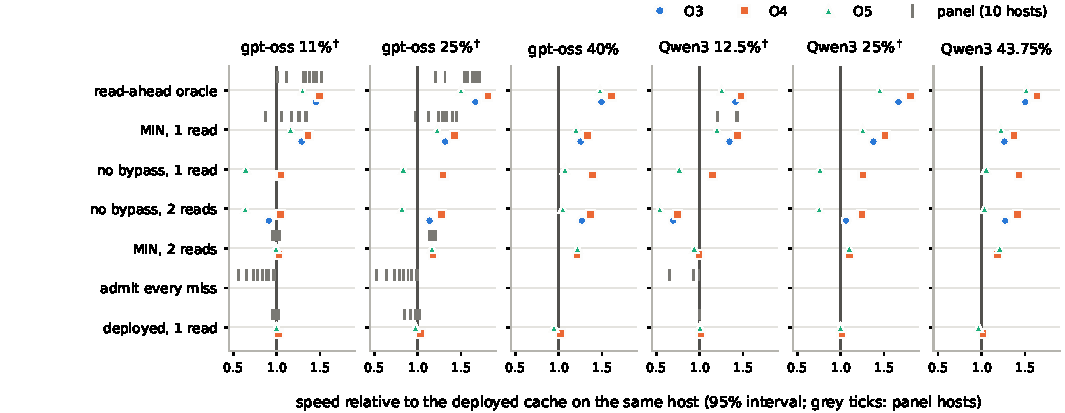
\includegraphics[width=\textwidth]{figs/factorial.pdf}
\caption{What foresight is worth in the engine, by how it is spent: speed of each configuration of \cref{tab:configs}
relative to the deployed cache on the same host, at the six budgets ($^\dagger$host-bound). Hosts O3 (job 095), O4 and
O5 (job 096, randomised order; O4's machine again in job 097) and O6 (job 097) at every budget; the \pnHosts{} panel
hosts (job 099, grey ticks) at the two gpt-oss host-bound budgets, and \pnHostsQlow{} of them at Qwen3 12.5\%. Within-host 95\% intervals are mostly narrower than the markers. On these hosts admitting what MIN
admits and reading it once (\emph{MIN, 1 read}) gains at every budget; the usual ways of spending foresight
(\emph{Belady}, \emph{MIN, 2 reads}) gain at some budgets and lose at others. Panel hosts whose link is much slower
than their CPU are the exception (\cref{fig:hostdep}).}
\label{fig:factorial}
\end{figure*}

\paragraph{Spent as the optimum spends it, foresight pays.} On hosts O3--O5, MIN with each admission fetched once in
the step runs \fxFetchAllGainMin--\fxFetchAllGainMax\% faster than the deployed cache at every budget,
and its reads are within \fxFetchSimDiffMax\% of what the trace simulator predicts. Copying its admissions three steps
ahead adds the overlap foresight allows: \fxPacedAllGainMin--\fxPacedAllGainMax\% over the deployed cache, which brings
the engine to \fxBestFracMin--\fxBestFracMax\% of the bound at the host-bound budgets.

\paragraph{Spent the usual ways, it pays less and sometimes loses.} Two habits waste foresight. A Belady prefetch
admits every expert the coming steps request, including those MIN would bypass, and reads
\fxNbReadsOverOptMin--\fxNbReadsOverOptMax$\times$ MIN's bytes even when each admission is read once. Serving a miss on
the CPU and then copying it reads every admission twice. At the two smallest budgets the best of these runs
\fxUsualLowMin--\fxUsualLowMax$\times$ the deployed cache on O4 and O5, against \fxFetchLowMin--\fxFetchLowMax$\times$ for
MIN with one read; at every host-bound budget MIN with its admissions copied ahead beats the best usual way by
\fxMinOverUsualMin--\fxMinOverUsualMax$\times$. The same trade-off between prefetching what an optimum would bypass and
admitting conservatively is classical for disks~\cite{cao1995prefetching} and CPU caches, where a Belady-style prefetch
also costs 75\% more traffic than MIN~\cite{jain2018prefetch}.

\paragraph{The machine decides which load pays.} Fetching an admission in the step puts its read on the PCIe link and
on the critical path. The panel adds hosts whose link reads much more slowly than their CPU (\cref{fig:hostdep}). On
them MIN with one read in the step gains less, and on the host with the lowest link-to-CPU ratio, a Core Ultra 9 285K
whose link reads at \hdRatioMin{} of its CPU rate, it loses (\hdFetchMin$\times$ at gpt-oss 11\%); another host with
the same CPU model, a faster link and a slower CPU path, gains. Across \hdHosts{} hosts the gain tracks the logarithm
of the link-to-CPU ratio (correlation \hdFetchCorrLow{} at 11\% and \hdFetchCorrMid{} at 25\%), mostly through the two
slow-link hosts: among the others it is \hdFetchCorrFastLow{} and \hdFetchCorrFastMid. Copied ahead of use instead,
the same admissions never lose (\hdPacedMin--\hdPacedMax$\times$; the lowest-ratio host breaks even at 11\%).
Admitting every miss, which sends every read over the link, runs \hdAaMin--\hdAaMax$\times$ the deployed cache: near
parity only where the link alone reads nearly as fast as CPU and link together.

What predicts the sign is the calibrated time model of \cref{app:law},
$T = G + \max(X_c/B_c,\ X_p/B_p,\ (X_c{+}X_p)/B_{cp})$: the three rates from the host's probe, the bytes the CPU and the
link read from the state's counters, and $G$, the GPU's work and the step's fixed costs, frozen per budget at the
median of the other hosts' fits (the fits range from \hmGMin{} to \hmGMax\,ms). It predicts the time of every state
that reads in the step, the deployed state's included, within a median \hmFrozenStepMed\% (90th percentile
\hmFrozenStepPninety\%) on \hmHostCells{} host-budgets of \hmHostsN{} hosts, and whether MIN with one read in the step
beats the deployed cache at all \hmFetchN{} of them. We then tested it on \jaHosts{} further launches from the probe
alone (job 100): before any timed run, each host wrote the predicted time of the four states that read in the step and
whose counts do not depend on the host. Over \jaProbeN{} predictions the median error is \jaProbeMed\%; the largest,
\jaProbeMax\%, under-predicts MIN with one read on the slow-link host, where copies in the step share host memory less
evenly than the probe's combined rate says (\cref{app:law}). A model with one read path (all host bytes at the best probed
rate) gets \hmFetchSignOnePath{} right: it misses both losses. The model predicts every state whose copies run in the
background faster than it runs (median \hmFrozenBgMed\%, \hmFrozenBgN{} host-budget-states): those copies are not free.
So the probe's two read rates say how a cache should spend foresight on a given machine; \cref{sec:limits} says where
this was tested.

\begin{figure*}[t]\centering
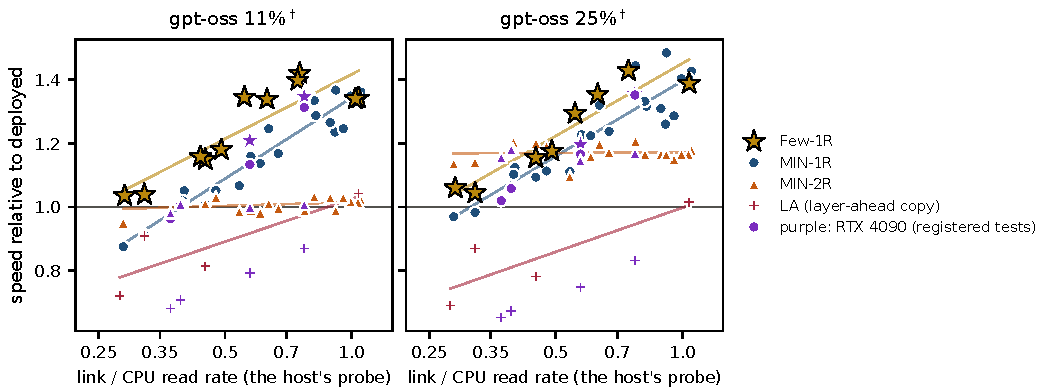
\includegraphics[width=\textwidth]{figs/hostdep.pdf}
\caption{Which way of spending foresight pays depends on the machine: speed relative to the deployed cache on the same
host against the host's link-to-CPU read-rate ratio from its own probe, at the two gpt-oss host-bound budgets, on hosts
O3--O6 and the panel. Lines: least-squares fits in the log of the ratio, for the trend only.}
\label{fig:hostdep}
\end{figure*}

% generated by scripts/factorial_shapley.py
\begin{table*}[t]\centering\footnotesize
\caption{An order-free accounting of the gap between the deployed cache and the bound at the host-bound budgets, as
percentages of the gap (ms per token). The engine ran both choices of what to cache (the deployed policy's admissions
or MIN's) with both ways to load a cached expert (two reads: the CPU serves it, then a copy; one read: a copy in the
step). \emph{Load alone} and \emph{cache alone} are each choice's effect with the other at the deployed level; the
\emph{interaction} is how much more MIN's set is worth loaded once than loaded twice. The Shapley values average each
choice's effect over the other's two levels and add up, with the prefetch (nested under MIN's set, since it needs
foresight) and the rest, to 100\%. Panel: mean over its hosts (number
in parentheses) and, in small type, the range over its hosts (not an interval); a fast link reads at least half as fast as
the host's CPU, a slow one less. Last rows: the new machines of the follow-up launches, with their link-to-CPU ratio.}\label{tab:shapley}
\setlength\tabcolsep{3pt}\resizebox{\textwidth}{!}{%
\begin{tabular}{llrrrrrrrr}\toprule
 & & Gap & Load & Cache & Inter- & \multicolumn{2}{c}{Shapley value} & Prefetch & Rest \\
Host & Budget & (ms) & alone & alone & action & cache & load & & \\\midrule
O4 & gpt-oss 11\% & 10.6 & 4 & 4 & 43 & 26 & 25 & 13 & 36 \\
O4 & gpt-oss 25\% & 8.5 & 4 & 22 & 17 & 31 & 13 & 22 & 34 \\
O4 & Qwen3 12.5\% & 18.4 & 3 & $-$1 & 58 & 28 & 32 & 4 & 36 \\
O4 & Qwen3 25\% & 14.1 & 2 & 14 & 37 & 33 & 21 & 17 & 30 \\
O5 & gpt-oss 11\% & 11.4 & 0 & $-$2 & 28 & 12 & 14 & 17 & 57 \\
O5 & gpt-oss 25\% & 9.1 & $-$4 & 20 & 10 & 25 & 1 & 21 & 52 \\
O5 & Qwen3 12.5\% & 19.8 & 1 & $-$13 & 43 & 9 & 23 & 7 & 62 \\
O5 & Qwen3 25\% & 15.3 & 0 & 14 & 17 & 22 & 9 & 16 & 53 \\
\midrule
Panel, fast link (8) & gpt-oss 11\% & 11.6 & 1 {\scriptsize($-$2 to 4)} & 3 {\scriptsize($-$2 to 6)} & 38 {\scriptsize(30 to 47)} & 22 {\scriptsize(14 to 26)} & 20 {\scriptsize(14 to 27)} & 13 {\scriptsize($-$4 to 20)} & 45 {\scriptsize(38 to 55)} \\
Panel, fast link (8) & gpt-oss 25\% & 9.0 & 0 {\scriptsize($-$4 to 3)} & 22 {\scriptsize(18 to 26)} & 15 {\scriptsize(10 to 19)} & 29 {\scriptsize(25 to 35)} & 8 {\scriptsize(1 to 12)} & 20 {\scriptsize(9 to 23)} & 43 {\scriptsize(38 to 49)} \\
Panel, slow link (2) & gpt-oss 11\% & 9.7 & $-$6 {\scriptsize($-$9 to $-$3)} & $-$4 {\scriptsize($-$9 to 0)} & 3 {\scriptsize($-$6 to 11)} & $-$3 {\scriptsize($-$11 to 6)} & $-$5 {\scriptsize($-$12 to 2)} & 17 {\scriptsize(9 to 24)} & 91 {\scriptsize(83 to 99)} \\
Panel, slow link (2) & gpt-oss 25\% & 7.8 & $-$17 {\scriptsize($-$22 to $-$11)} & 19 {\scriptsize(16 to 23)} & 3 {\scriptsize(3 to 3)} & 21 {\scriptsize(17 to 25)} & $-$15 {\scriptsize($-$21 to $-$10)} & 22 {\scriptsize(17 to 26)} & 73 {\scriptsize(68 to 78)} \\
\midrule
5700X3D (0.92) & gpt-oss 11\% & 14.9 & 4 & $-$2 & 55 & 25 & 31 & 8 & 36 \\
5700X3D (0.92) & gpt-oss 25\% & 11.5 & 4 & 22 & 24 & 34 & 17 & 18 & 31 \\
9950X, x8 (0.54) & gpt-oss 11\% & 8.3 & 0 & $-$3 & 17 & 5 & 8 & 28 & 59 \\
9950X, x8 (0.54) & gpt-oss 25\% & 7.4 & $-$15 & 13 & 17 & 22 & $-$6 & 26 & 59 \\
9800X3D, slower link (0.61) & gpt-oss 11\% & 10.8 & $-$2 & $-$4 & 29 & 11 & 12 & 20 & 57 \\
9800X3D, slower link (0.61) & gpt-oss 25\% & 8.9 & $-$5 & 20 & 12 & 26 & 1 & 20 & 54 \\
\bottomrule\end{tabular}}\end{table*}


\paragraph{An order-free accounting.} Two choices separate the deployed cache from MIN with one read in the step:
\emph{what to cache} (the deployed policy's admissions or MIN's) and \emph{how to load} a cached expert (served by the
CPU and then copied in the background, two reads; or copied in the step, one read). The engine ran all four
combinations on O4, O5 and the panel. Take O4 at gpt-oss 11\%, \fsExGap\,ms per token from the bound. Changing only
what to cache closes \fsExSetTwo\% of that gap; changing only how to load closes \fsExReadsOnline\%; changing both
closes \fsExBoth\%. The extra \fsExInter{} points are an interaction: MIN caches
\fxMinAdmitsOverOnlineMin--\fxMinAdmitsOverOnlineMax{} times as many experts per token as the deployed policy, and
loaded the deployed way each of them is read twice, the second time on the critical path; the deployed policy caches a
few experts per token, and their background copies overlap later steps. Because each choice's effect depends on the
other, we credit each with its effect averaged over the two orders, its Shapley
value~\cite{fawcett2016ablation,jain1991art}: \fsExSet\% and \fsExReads\% here. Splitting the interaction equally is a
convention, so \cref{tab:shapley} also gives each choice alone and the interaction. Copying MIN's admissions ahead of
use needs foresight by construction, so it is nested under MIN's set rather than crossed (\fsExPacing\% here); what no
oracle touches is the rest (\fsExRest\%). Only the two crossed choices are order-free.

On the \fsBalHosts{} hosts whose link reads at least half as fast as their CPU, either choice alone is worth
\fsBalSetTwoMin{} to \fsBalSetTwoMax\% of the gap, the interaction \fsBalInterMin--\fsBalInterMax\%, and both
together \fsBalBothMin--\fsBalBothMax\%. The Shapley values are \fsBalSetMin--\fsBalSetMax\% for what to cache and
\fsBalReadsMin--\fsBalReadsMax\% for how to load; prefetching adds \fsBalPacingMin{} to \fsBalPacingMax\%, and the
rest is \fsBalRestMin--\fsBalRestMax\%. On the \fsSlowHosts{} hosts whose link reads at less than half their CPU's rate,
loading in the step costs time at \fsSlowReadsLoseN{} of \fsSlowCells{} host-budgets (Shapley value \fsSlowReadsMin{} to
\fsSlowReadsMax\%), and the rest is \fsSlowRestMin--\fsSlowRestMax\% of the gap. We drew the line at half after the
panel ran; the model above, not the line, carries the prediction.

\paragraph{The rest.} Three things are visible in it. The prefetch is imprecise: it reads
\fsbpReadsOptMin--\fsbpReadsOptMax$\times$ MIN's bytes, from victims chosen steps early and from misses inside the lead.
The overlap is partial: a model that charges every host read in sequence with the GPU's work over-predicts the
prefetching state's time by \fxPacedLawTimeMin{} to \fxPacedLawTimeMax\%, so some reads overlap and some do not. And
the GPU runs at about half of its datasheet rate at batch size 1, which is most of what remains at the GPU-bound budgets
(\cref{app:foresight}). The rest grows as the link slows relative to the CPU, because the bound lets the two paths
share the host's read rate freely while any cache that fetches must put some reads on the link.

\paragraph{Machines differ more than problems.} On the panel, the within-host 95\% interval of MIN-with-one-read's
gain has a median half-width of \pnFetchLowHw{} at gpt-oss 11\%, while its standard deviation across hosts is
\pnFetchLowSd; the two-stage interval over hosts is [\pnFetchLowLo, \pnFetchLowHi]. Part of that spread follows the
link-to-CPU ratio (\cref{fig:hostdep}) and part does not. Launches of one machine agree: a relaunch of O4's
machine reproduced its ratios within \fxReplicateMax, and relaunches of two panel machines every ratio within
\jaRelaunchRatioMax{} and the deployed cache's time within \jaRelaunchBaseMax\%. The machine, not the launch or the
problem, is the unit of variation. Statements in this section are therefore about orderings that hold on every host of a stated class,
and about a model that predicts each host.

\section{How Much Foresight Is Needed}\label{sec:horizon}
The oracles know the whole future. A forecaster would know part of it, imperfectly. We measure the value of partial
foresight in two ways: in the engine on the panel, and on routing traces of nine models.

\paragraph{In the engine.} The panel ran a family of policies between \emph{admit every miss} and MIN (\cref{tab:configs}):
the victim is the lowest-scored resident not seen in the next $W$ tokens' routing, or, if every resident is seen, the
one seen furthest ahead, and a miss is admitted unless the window says the victim is needed sooner. With no window this
is admitting every miss, the best online policy in reads at these budgets (below); with the whole rest of the problem
in view it is MIN. Every admission is copied in the step, as in admit-every-miss. We also degraded the window:
each future expert is kept with probability $r$ and otherwise replaced by a random one, so precision and recall are
both $r$, with errors drawn independently for every step at which the window is consulted. The engine plans each step
on the host before the step, exactly as a replay script does (equal on a CPU build at three budgets, within
\pnReplayMax\% on the panel's GPUs). \Cref{fig:value} gives the share of MIN's gain over admitting every miss that each window
recovers, in time on the panel and in reads on the trace.

\begin{figure*}[t]\centering
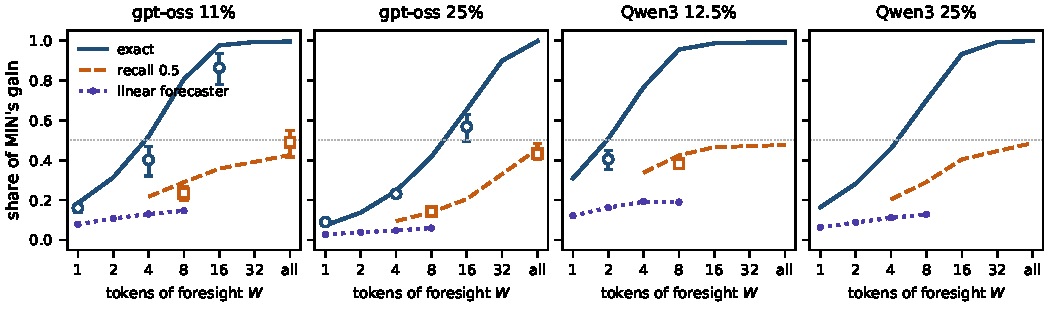
\includegraphics[width=\textwidth]{figs/value.pdf}
\caption{The value of partial foresight at the four host-bound budgets: the share of MIN's gain over \emph{admit every
miss} recovered by exact routing of the next $W$ tokens (solid), by a window whose experts are each right with
probability 0.5 (dashed), and by a linear forecaster fitted on other text (dotted), in host reads on the AIME routing
the engine runs; markers: the same share in time per token on the panel hosts (mean, and range over hosts; \pnHostsLow{} hosts
for gpt-oss, \pnHostsQlow{} for Qwen3 at 12.5\%; no Qwen3 run at 25\%). The grey line marks half of the gain.}
\label{fig:value}
\end{figure*}

At gpt-oss 11\%, exact foresight of 1, 4 and 16 tokens recovers \pnShareOneLowMin--\pnShareOneLowMax,
\pnShareFourLowMin--\pnShareFourLowMax{} and \pnShareSixteenLowMin--\pnShareSixteenLowMax{} of the gain in time across
hosts; at 25\%, where the cache turns over more slowly, \pnShareFourMidMin--\pnShareFourMidMax{} at 4 tokens and
\pnShareSixteenMidMin--\pnShareSixteenMidMax{} at 16. A window saves host reads but, like the policy it extends, still
copies almost every miss over PCIe during the step. At 11\% a 4-token window removes \pnReadFourLowMin{} of the reads
MIN removes, yet \pnLinkPctFour\% of its remaining misses cross the link on the critical path, against
\pnLinkPctMin\% of MIN's. Where the link is slower than the CPU's own reads, the window therefore saves less time than
its read savings suggest: a share \pnGapFourLowMin{} lower on hosts whose two paths are equally fast, and
\pnGapFourLowMax{} lower on the host whose link reads at \pnGapRatioAtMax{} of its CPU rate (correlation with the log
ratio \pnGapFourCorr). The calibrated model predicts the exact windows' shares of the time gain within
\hmWinShareErrMed{} (median over the \hmWinShareN{} host-budget-windows; at most \hmWinShareErrMax). Measured against
the deployed cache rather than against admitting every miss, the same windows often lose: a 4-token window is slower
than the deployed cache on \pnSlowerFourLow{} of \pnHostsLow{} hosts at 11\% (\pnSlowerFourMid{} at 25\%), a 16-token
window on \pnSlowerSixteenLow{} (\pnSlowerSixteenMid).

% generated by scripts/job100.py
\begin{table}[t]\centering\footnotesize
\caption{Foresight on each read path (job 100): speed relative to the deployed cache on the same host. \emph{In step}:
admit every miss with a window of $W$ exact tokens, each admission copied in the step (as on the panel). \emph{Deployed
path}: the deployed policy with the same window, its misses split between the CPU and an in-step copy by the host's
fetch table and its admissions copied in the background;
$W{=}8$ at recall 0.5 in the column marked $r$. Hosts sorted by the probe's link-to-CPU ratio.}\label{tab:window100}
\setlength\tabcolsep{2.5pt}\resizebox{\linewidth}{!}{%
\begin{tabular}{@{}lrlrrrrrrrr@{}}\toprule
 & Link/ & & \multicolumn{2}{c}{In step} & \multicolumn{3}{c}{Deployed path} & MIN, & MIN, & MIN, \\
Host & CPU & Budget & $W{=}4$ & 16 & 4 & 16 & $r$ & 2 reads & 1 read & pref. \\\midrule
Pd again & 0.41 & gpt-oss 11\% & 0.66 & 0.89 & 1.02 & 1.03 & 0.94 & 1.00 & 1.05 & 1.11 \\
Pd again & 0.41 & gpt-oss 25\% & 0.69 & 0.81 & 1.03 & 1.12 & 1.01 & 1.19 & 1.11 & 1.29 \\
9950X, slower link & 0.54 & gpt-oss 11\% & 0.65 & 0.89 & 1.01 & 1.01 & 0.96 & 0.99 & 1.07 & 1.23 \\
9950X, slower link & 0.54 & gpt-oss 25\% & 0.69 & 0.80 & 0.96 & 1.06 & 1.00 & 1.10 & 1.11 & 1.37 \\
5700X3D & 0.92 & gpt-oss 11\% & 1.09 & 1.32 & 0.99 & 1.00 & 0.95 & 0.99 & 1.37 & 1.44 \\
5700X3D & 0.92 & gpt-oss 25\% & 1.06 & 1.23 & 1.03 & 1.07 & 1.00 & 1.16 & 1.48 & 1.80 \\
Ph again & 0.96 & gpt-oss 11\% & 0.99 & 1.20 & 1.01 & 1.03 & 0.98 & 1.03 & 1.27 & 1.45 \\
Ph again & 0.96 & gpt-oss 25\% & 0.97 & 1.09 & 1.03 & 1.07 & 1.01 & 1.16 & 1.29 & 1.64 \\
\bottomrule\end{tabular}}\end{table}


\paragraph{On the deployed path.} Job 100 gave the same windows to the deployed policy instead (\emph{deployed +
window} in \cref{tab:configs}): the CPU serves every miss and admissions are copied in the background, so foresight
changes only what is cached. On \jaHosts{} hosts (\cref{tab:window100}; two panel machines relaunched and two new,
link-to-CPU ratios \jaRatioMin--\jaRatioMax) this spend is safe but small: a 16-token window runs
\jaBSixteenLowMin--\jaBSixteenLowMax$\times$ the deployed cache at gpt-oss 11\% and
\jaBSixteenMidMin--\jaBSixteenMidMax$\times$ at 25\%, never more than \jaBSixteenOverBypassMax{} above MIN with two
reads. Its admissions land steps after they are issued, so the engine misses \jaReplayDevMin--\jaReplayDevMax\% more
than a replay that admits at once. Which path pays depends on the host, as for MIN: at 16 tokens the deployed path
wins on the slow-link host and the in-step path on the hosts whose link matches the CPU. Only MIN with its copies made
ahead never loses.

Accuracy matters as much as horizon. With each foreseen expert right only half the time, a window of 8 tokens recovers
\pnShareEightHalfLowMin--\pnShareEightHalfLowMax{} at 11\% (in reads about what 2 exact tokens buy; on Qwen3 at 12.5\%,
where the engine ran both, \pnShareEightHalfQlowMin--\pnShareEightHalfQlowMax{} against
\pnShareTwoQlowMin--\pnShareTwoQlowMax), and the whole future \pnShareAllHalfLowMin--\pnShareAllHalfLowMax. For the
whole future the model over-predicts the share by up to \hmAllHalfOverMax{} on fast-link hosts, which we have not
explained; planning costs at most \SI{\pnPlanMaxLow}{\micro\second} per step, too little to account for it. On the
traces, dropping experts without replacing them (recall $r$, precision 1) costs about the same as replacing them for
windows of up to 16 tokens, and less with the whole future in view at low recall (\cref{app:value}).

\paragraph{On the traces of nine models.} The trace study replays each model's own sampled text (33{,}000--152{,}000
tokens per model) through an event-level simulator in which a token requests its $k$ experts per layer as one set and
no expert of the current token is evicted to serve it~\cite{zhang2026reproducible}. Adding \emph{admit every miss} to
the online policies changes their ranking: it reads least of LRU, LFU, two decayed-frequency variants, ARC, S3-FIFO and
itself in \rbPolAaWins{} of \rbPolCells{} budget points (\rbPolAaTies{} ties), and at most \rbPolAaLossMax\% more where
it loses. Even so, the best online policy reads \rbPolBestMin--\rbPolBestMax\% more than MIN (\cref{tab:policy},
\cref{app:traces}). Against this stronger baseline, the window that closes half of the read gap grows with the
cache's turnover time $C/k$ as $W_{50}\approx\rbPre\,(C/k)^{\rbExp}$ tokens ($r{=}\rbR$ over \rbAaCells{} points; the exponent's
95\% interval over a bootstrap of models is \rbExpLo--\rbExpHi, and \rbExpNoInterp{} without the points below one
token).

\paragraph{The horizon in distinct experts.} A power law in tokens hides why the horizon differs between models. Paging
theory measures lookahead in distinct future pages, not requests~\cite{albers1997lookahead,breslauer1995lookahead}. Let
$D(W)$ be the mean number of distinct experts a layer requests in a window of $W$ tokens. At every point of the fit,
$D(W_{50})$ is close to a fixed fraction of the cache: median \dcMed$\,C$ (quartiles \dcLo--\dcHi, coefficient of
variation \dcCv), while $W_{50}$ itself ranges from \dcWMin{} to \dcWMax{} tokens. The models differ in how fast
$D(W)$ grows ($D\propto W^\beta$ with $\beta$ from \dcBetaMin{} to \dcBetaMax), which is why the exponent in tokens
wanders. Fitted on eight models and tested on the ninth, the rule ``$D(W_{50}) = c\,C$'' predicts the held-out model's
horizon about as well as the power law, with one constant instead of two, and better than $W_{50}\propto C/k$
(\cref{tab:lomo}); over a bootstrap of models the ratio of the power law's median error to the rule's is
\dbRatioLo--\dbRatioHi, so the two are not distinguished. Within a model the fraction falls as the cache grows (from
the smallest budget to the largest in \dbTrendDown{} of \dbTrendModels{} models), so $c$ is an average over budgets.
What the rule adds is the unit: a forecaster's target is stated in quantities it controls, the next
$\approx$\dcMed$\,C$ distinct experts of each layer.

% generated by scripts/w50_rebaseline.py
\begin{table}[t]\centering\footnotesize
\caption{Predicting a held-out model's horizon $W_{50}$ (fitted on the other eight models, tested on the ninth, over all
\rbAaCells{} budget points): error as a factor, $\max(\hat W/W, W/\hat W)$.}\label{tab:lomo}
\begin{tabular}{@{}lrrrr@{}}\toprule
Rule & Constants & Median & 90th pct. & Max \\\midrule
$W_{50}\propto C/k$ & 1 & 1.22 & 1.57 & 2.42 \\
$W_{50}=a\,(C/k)^b$ & 2 & 1.19 & 1.51 & 1.67 \\
$D(W_{50})=c\,C$ & 1, and $D(W)$ & 1.16 & 1.42 & 1.61 \\
\bottomrule\end{tabular}\end{table}


\paragraph{What could supply it.} We know of no realisable source of routing foresight that reaches this horizon.
\emph{Online policies} cannot (above). \emph{A learned admission order} fitted on other text, with features the engine
has when it plans a step, reads \lreFewerMin--\lreFewerMax\% fewer experts in the engine than the deployed policy with
single reads, but runs \lreOverBaseMin--\lreOverBaseMax$\times$ the deployed cache at the host-bound budgets; on the
trace, admitting every miss alone gets most of its read saving on Qwen3 (\cref{app:traces}). \emph{Speculative
batches} request a layer's experts for $K$ draft positions at once; once the rejected drafts' experts are counted, they
save an online cache \bkSameNineMin--\bkSameNineMax\% of its reads at 90\% acceptance and cost
\bkSameEightLossMin--\bkSameEightLossMax\% at 80\%~\cite{spmoe,moespac2026,cascade2025}. \emph{Layer-ahead predictors}
apply the next layer's router to the current hidden state~\cite{hwang2024pregated,zhu2025preattention}; they reach
\laRecallK\% recall at $k$ and \laRecallEight\% with 8 candidates on gpt-oss in our engine, but see less
than one token ahead. \emph{Forecasters} trained on routing histories
are the remaining candidate. A linear forecaster we fitted on each model's other text forecasts gpt-oss's experts with a
precision of \lfPrecOneGpt{} one token ahead and \lfPrecFourGpt{} four ahead, and closes \lfShareMinGpt--\lfShareMaxGpt\%
of the read gap (\lfShareMinQwen--\lfShareMaxQwen\% on Qwen3; \cref{fig:value}, dotted). Its precision falls with the
horizon, and over a window it closes no more than a window with random errors of the same average precision; on Qwen3
less, because the experts it gets right are mostly ones the cache already holds. A
sequence model reports 90\% recall one token ahead on both of our models with $k{+}3$ candidates~\cite{wang2026seqmoe};
a recurrent model of the same inputs that we trained the same way as the linear one reaches \grRecThreeGpt{} on
gpt-oss and \grRecThreeQwen{} on Qwen3 by that measure, and closes no more of the gap (\cref{app:value}).

\section{Related Work}\label{sec:related}
\paragraph{Offloading systems.} Demand-paging systems cache experts per layer and copy misses over
PCIe~\cite{eliseev2023offloading,xue2024moeinfinity,song2024promoe,tang2024hobbit,pagingexperts2026}; an upstream
llama.cpp pull request adds such a cache, admitting every miss into an LRU~\cite{llamacpppr29887}. CPU-execution
systems run non-resident experts on the host~\cite{kamahori2024fiddler,ktransformers,zhong2025hybrimoe,daop2025,wang2026cloudgrade,atsinfer2026};
a set-associative GPU cache with CPU-executed misses~\cite{huang2025cpugpu}, a llama.cpp fork~\cite{leloch2026,llamacppdisc24528}
and two llama.cpp pull requests~\cite{llamacpppr26563,llamacpppr27861} are the closest designs to ours.
FreeToken~\cite{freetoken} and DALI~\cite{dali2026} split each layer's misses between CPU and PCIe. Predictors guess
upcoming experts from the previous layer's state~\cite{hwang2024pregated,zhu2025preattention}, several tokens ahead
with a learned forecaster~\cite{wang2026seqmoe,mira2026}, or from draft tokens~\cite{spmoe,moespac2026,cascade2025};
Read-ME decouples the router so routing is known in advance~\cite{readme2024}. Batched-throughput
systems~\cite{flexgen2023,cao2024moelightning,yuan2025moelens} and SSD tiers~\cite{ssdllama,edgezero} are outside our
scope.

\paragraph{Bounds, oracles and caching theory.} WiSP~\cite{wisp2026} bounds decode by PCIe turnover, Budgeting
Bytes~\cite{budgetingbytes2026} by bytes over bandwidth for a given fetch set, and MoE-CAP~\cite{moecap} measures
bandwidth utilisation against a single peak; the roofline~\cite{williams2009roofline} is the single-memory ancestor of
our bound. Zhang~\cite{zhang2026reproducible} proposes a trace-level evaluation contract and reports a 44--46\% gap
between causal policies and MIN with bypass; Liang et al.~\cite{liang2026lrc} measure, across 20 models, the hit rate
of an oracle cache that sees $m$ tokens ahead against the cache ratio $C/k$. We add the time domain: an oracle inside a
real engine, the cost of how foresight is spent, and a horizon rule that predicts held-out models. SAEM~\cite{saem2026}
gives its own stage-level planner perfect knowledge of the coming stage in its engine and finds that worth at most
about 14\% on an A100; SpecMD~\cite{specmd} benchmarks expert-cache and speculative prefetch policies across hardware; Angelopoulos et
al.~\cite{angelopoulos2025cache} give competitive bounds for layered expert paging. With bypass, MIN maximises hits
exactly~\cite{carlisle1995kcoloring,jain2016hawkeye}; when bypass and admission cost differ, the time-optimal placement
is a different problem~\cite{chopt2020}, which is why we use MIN's reads as an input to a bound rather than as a
time-optimal policy. Lookahead in paging is valuable when measured in distinct pages~\cite{albers1997lookahead,breslauer1995lookahead},
and learning-augmented paging is most robust with predictions of whether a page will be evicted before its next
use~\cite{antoniadis2023succinct}; learned replacement imitates Belady in CPU and content-delivery
caches~\cite{jain2016hawkeye,song2020lrb} and in an SSD-backed expert cache~\cite{flashmoe2026}.

\section{Limitations}\label{sec:limits}
\begin{itemize}\setlength\itemsep{1pt}
\item \textbf{Hardware.} Rented consumer cards (RTX 5090 for the headline, a 4090 and a 3090 in \cref{app:grid}) in
desktop hosts; GPU clocks could not be locked and power limits differed. The panel covers \pnHosts{} hosts of several
CPU classes, one launch each (two relaunched, with two new hosts, in job 100), at two gpt-oss budgets (Qwen3 at one
budget on three); the crossed 2$\times$2 ran at
every budget on two hosts. Only \fsSlowHosts{} panel hosts have a link slower than half their CPU rate, so the
crossover in \cref{fig:hostdep} rests on few points; the calibrated model, not the fit, carries the prediction there.
That line at half was drawn after the panel ran; the panel's pre-registered classes were by absolute link rate.
\item \textbf{Workload.} Batch-1 decode of two models on AIME prompts, which were also used while developing the
system; teacher-forced on each model's own greedy text; the panel ran the first \pnProblems. Prompts and batches
above one bypass the cache.
\item \textbf{The bound.} Exact routing and per-layer slots only; pooling slots across layers lowers MIN's reads by
\globalReadsMin--\globalReadsMax\%. It drops latencies and lets the two read paths share the host's best probed rate
freely, so it is optimistic, and a faster reader than our probe could exceed it. We have not shown it can be reached:
the best oracle comes to \fxBestFracMin--\fxBestFracMax\% of it, and part of what we call the rest may be slack in the
bound rather than time a cache could save.
\item \textbf{The time model.} Its one constant per budget is fitted on other hosts; with the constants of the original
blind test frozen, it over-predicts Qwen3's speed on later hosts by \lawFrozenQwenMin{} to \lawFrozenQwenMax\%
(\cref{app:law}). It takes background copies as free, which they are not, and it fails on a 12-channel server host,
where a per-layer latency floor, not memory, binds.
\item \textbf{The oracles and the degraded windows.} Oracles read a recorded trace. Degraded windows draw errors
uniformly and independently; a real forecaster's errors are correlated with what the cache already knows, so the
value of a forecaster at a given precision and recall can be lower than \cref{fig:value} shows. The windows of the
panel extend admitting every miss and copy each admission in the step, which is the wrong path on slow-link hosts;
on the deployed path the same windows gain little anywhere (job 100, four hosts).
\item \textbf{Outputs.} Parity is measured by teacher-forced KL divergence and agreement against an all-VRAM reference
(mean KL \klMeanGpt{} and \klMeanQwen{} nats), not by task accuracy.
\end{itemize}

\section{Conclusion}
With experts in host memory, batch-1 MoE decode is bound by host bytes, and the bound is far from reached: our cache
reaches \bothLimitPctMin--\bothLimitPctMax\% of it, and by one common procedure published systems reach a median of
\audInclassMed\% and ours \audOursMed\%. Knowing the future recovers part of the gap when it is spent as MIN spends
it, caching only what MIN caches and loading each expert once on a path with room: on hosts whose link is not much
slower than their CPU, \fsBalBothMin--\fsBalBothMax\% of the gap. Which path has room is a property of the machine that
its two read rates predict. The rest of the gap, \fsBalRestMin--\fsBalRestMax\% on those hosts, is an imprecise
prefetch, partial overlap and a GPU at half its datasheet rate, and possibly slack in the bound. And foresight has a measurable price: about \dcMed$\,C$ distinct experts of each layer's coming routing, a few
to tens of tokens ahead, at accuracies no forecaster we know of or trained reaches. That is the target for the next MoE
cache, and for router designs that would make routing predictable in advance.

{\small\bibliographystyle{plain}\bibliography{refs,refs_wsg}}

\clearpage
\onecolumn
\appendix
\section{Scientific benchmarking checklist}\label{app:rules}
How this paper follows the twelve rules of Hoefler and Belli~\cite{hoefler2015benchmarking}.

\begin{longtable}{p{0.32\textwidth}p{0.61\textwidth}}\toprule
Rule & Where and how \\\midrule\endhead
1. Report the base case of a speed-up and its absolute performance. & Every ratio in \cref{tab:headline} is next to both absolute speeds; llama.cpp is configured with per-layer expert offload at equal expert memory, the setting its users run. \\
2. Explain subsets of benchmarks or resources. & Two models chosen for size and precision (MXFP4, BF16), a third that is FreeToken's own headline model; budgets span what fits a 32\,GB card; the 43.75\% budget is omitted where it does not fit. All 30 AIME-25 problems are used. \\
3. Arithmetic mean for costs, harmonic mean for rates. & Every problem decodes the same number of tokens, so the harmonic mean of rates is total tokens over total time; ratios of total time agree with the reported ratios of mean rates within 0.003. \\
4. Avoid summarising ratios. & Ratios are computed from mean speeds, never averaged across budgets or models; ranges list the per-budget values. \\
5. Report whether measurements are deterministic; give confidence intervals. & Decode is greedy and deterministic per engine; timing is not. Every comparison has a 95\% interval. \\
6. Do not assume normality. & Intervals are bootstrap percentile intervals (10{,}000 resamples, paired by problem); no distributional assumption. \\
7. Compare nondeterministic data soundly. & Paired bootstrap of the ratio of means; the variant a system is scored with is picked on a separate launch (except the Qwen3 25\% row of \cref{tab:headline}). \\
8. Check that central tendency is the right summary. & Mean speed over 256 tokens is FreeToken's own metric; per-token p50 and p99 latencies are recorded for every problem in the released rows. \\
9. Document all factors and the setup. & Machines, probes, power limits, memory clocks (\cref{sec:setting}), software commits (llama.cpp 4da6337, FreeToken 0d652e7), flags and job scripts are released; \cref{app:artifact}. \\
10. Report measurement, synchronisation and summarisation. & One client times every system from streamed token arrivals; no server-side timers enter a comparison (\cref{sec:setting}). \\
11. Show upper performance bounds. & The speed limit (\cref{sec:limit}) and all-in-VRAM speed are columns of \cref{tab:headline}; \cref{tab:limit} tightens the limit four ways; \cref{sec:audit} applies it to the published literature. \\
12. Plot enough to interpret; connect points only for trends. & \Cref{fig:shapley,fig:ablation} are bar charts; \cref{fig:ratio,fig:audit} are scatter plots; no interpolation. \\
\bottomrule
\end{longtable}

\section{Prediction log}\label{app:prereg}
Each job's predictions are in the header of its script on the public \texttt{gpu} branch, committed and pushed
before the machine started; git history orders every prediction before its measurement. Outcome notes with the
statistics are in \texttt{prereg/}. \Cref{tab:scorecard}, generated from \texttt{prereg/scorecard\_clauses.json},
splits every prediction of jobs 073--092 into its separable clauses and scores each under one rule: \emph{held} only
when the point estimate is on the predicted side and the 95\% paired-bootstrap interval excludes the threshold (for a
band, lies inside it); \emph{held (point)} when only the point estimate is, or no interval exists; \emph{failed} when
the point estimate is on the wrong side; \emph{untested} when the clause could not be evaluated; \emph{void} when the
job was voided. Of \scClauses{} clauses, \scHeld{} held, \scHeldPoint{} held on the point estimate, \scFailed{} failed,
\scUntested{} were untested and \scVoid{} void: \scEarlyHeld{} of \scEarlyScored{} scored clauses held in jobs 073--075,
when the system was being built, \scMidHeld{} of \scMidScored{} in jobs 076--081, \scMidSign{} of them sign-only predictions
made after a same-host pilot, \scLateHeld{} of \scLateScored{} in jobs 082--087, and \scRevHeld{} of \scRevScored{} in the jobs run after the
reviews (088 onward), where \scRevSignHeld{} of \scRevSignClauses{} sign clauses held and \scRevFailBand{} of
\scRevBandClauses{} bands failed. The bands that failed are the sizes of effects whose direction held: our slow-link
lead landed at 1.51--1.58$\times$ against a predicted 1.10--1.50; the rerun of \cref{tab:headline} on a second host
(job 089) gave ratios \scRatioFailMin--\scRatioFailMax{} below the headline machine's at \scRatioFailCells{} of six
cells against a predicted $\pm$0.06, host-bound speeds \scOursHybDropMin--\scOursHybDropMax\% lower against a
predicted $\pm$12\%, and LRU \scLruFailMin--\scLruFailMax\% slower than decayed frequency at the two GPU-heavy
cells against a predicted 10--30\%; on the 4090 and 3090 hosts (jobs 091, 092; \cref{app:grid}) our lead over
FreeToken and its fraction of the limit overshot their bands, FreeToken's carried-over backend fell far below its
band, and two launch-order checks exceeded 3\%. The \scRevFailThr{} threshold failures are ours at
1.56--1.78$\times$ llama.cpp on the slow hosts against a predicted 1.8 and the Mixtral tie against a predicted
1.3$\times$; the \scRevFailEq{} equality failures are the 4090 host's FETCH tables, which copy one more expert than
predicted; the one sign failure is LRU behind FreeToken at gpt-oss 11\%, where we predicted it would still lead.
Against the earlier draft's log, two clauses are downgraded (a llama.cpp clause of job 074b that the log counted as
held was never run; job 085b's own restatement of its fourth prediction, ``at least 2 of 3'', failed at 1 of 3,
though the pooled 4 of 6 held), job 073's ``identical outputs'' is scored on fully identical outputs (0--3\%) rather
than on agreement of the first 160 characters (27--47\%), and ten clauses the log counted as held, among them job
087's first, hold on the point estimate only under the interval rule; \texttt{prereg/scorecard\_outcome.md} lists
every change. Job 085's Qwen3 half ran as 085b on a second machine with a slow link after a hung conversion. Job 084 ran on
a throttled card and was rerun, with its predictions unchanged, as 084b/084c. The batched-verification variants of
\cref{sec:traces} (rejected drafts free, routed like the true token, or routed at random) are in
\texttt{prereg/batchk\_outcome.md}.

% Generated by scripts/scorecard.py from prereg/scorecard_clauses.json; do not edit by hand.
\begin{footnotesize}
\begin{longtable}{@{}p{0.08\textwidth}p{0.355\textwidth}p{0.07\textwidth}p{0.29\textwidth}p{0.10\textwidth}@{}}
\caption{Prediction scorecard, jobs 073--098: every committed prediction split into its separable clauses and scored under one rule. \emph{Held}: the point estimate is on the predicted side and the 95\% paired-bootstrap interval excludes the threshold (for a band, lies inside it). \emph{Held (point)}: the point estimate is on the predicted side but the interval includes the threshold, or no interval exists. \emph{Untested}: the clause could not be evaluated. \emph{Void}: the job was voided (084, a throttled card; its predictions are scored on 084b). Types: sign (a direction), threshold (a numeric bar), band (an interval), equality (a deterministic outcome). Measured values are ratios of mean speeds with 95\% intervals unless the clause says otherwise; \texttt{prereg/scorecard\_clauses.json} names the source of every number. Totals: 565 clauses, 218 held, 193 held (point), 142 failed, 8 untested, 4 void.}\label{tab:scorecard}\\
\toprule
Job & Clause & Type & Measured & Status \\\midrule
\endfirsthead
\toprule
Job & Clause & Type & Measured & Status \\\midrule
\endhead
\midrule\multicolumn{5}{r}{\emph{continued}}\\
\endfoot
\bottomrule
\endlastfoot
\multicolumn{5}{@{}l}{\textbf{Jobs 073--075}: 20 clauses, 7 held, 3 held (point), 9 failed, 1 untested, 0 void}\\
073 P1a & ours+FETCH $\ge$ 5\% ahead of FreeToken, 11\% & threshold & 1.109 [1.098, 1.120] & held \\
073 P1b & ours+FETCH $\ge$ 5\% ahead of FreeToken, 25\% & threshold & 1.084 [1.076, 1.092] & held \\
073 P1c & ours+FETCH within $\pm$5\% of FreeToken, 40\% & band & 0.941 [0.933, 0.951] & \textbf{failed} \\
073 P2 & ours+FETCH $\ge$ 1.8$\times$ llama.cpp, every budget & threshold & 1.832 [1.808, 1.856]; 2.358 [2.322, 2.396]; 2.647 [2.605, 2.686] & held \\
073 P3a & same-problem warm-up reads 5-15\% faster, the two caches & band & 0.991 [0.962, 1.028]; 0.997 [0.986, 1.008] & \textbf{failed} \\
073 P3b & same-problem warm-up within $\pm$2\%, llama.cpp & band & 0.962 [0.934, 0.979] & \textbf{failed} \\
073 P4 & $\ge$ 80\% of greedy outputs identical to llama.cpp's, every system & equality & ours (6 configurations): 0.000-0.033; FreeToken (6 configurations): 0.000; llama.cpp -ncmoe 32 / 22: 0.700 / 0.400 & \textbf{failed} \\
074 P1 & ec-bench launch time $\le$ 0.25 ms, C51 & threshold & 0.201 & held (point) \\
074 P2a & ours v2 $\ge$ 127 tok/s, C51 & threshold & 95.1 & \textbf{failed} \\
074 P2b & ours v2 ahead of FreeToken offload, C51 & sign & 0.831 [0.817, 0.845] & \textbf{failed} \\
074 P3a & ours v2 $\ge$ 59 tok/s, C14 & threshold & 41.5 & \textbf{failed} \\
074 P3b & ours v2 $\ge$ 91 tok/s, C32 & threshold & 65.3 & \textbf{failed} \\
074 P4 & half-life 64 within $\pm$2\% of half-life 16, C51 & band & 1.012 [0.997, 1.027] & held (point) \\
074b P1 & GPU sampling cuts between-step host time by $\ge$ 1 ms & threshold & 1.6 & held (point) \\
074b P2a & ours v2 $\ge$ 10\% faster with GPU sampling, C51 & threshold & 1.117 [1.109, 1.125] & held \\
074b P2b & stock llama.cpp $\ge$ 3\% faster with GPU sampling & threshold & -- & \emph{untested} \\
074b P3 & ours v2+FETCH with GPU sampling $\ge$ FreeToken offload, C51 & sign & 1.074 [1.063, 1.085] & held \\
075 P1 & ours ahead of FreeToken at 40\% (RTX PRO 6000) & sign & 1.122 [1.107, 1.137] & held \\
075 P2 & ours within -3 to +10\% of FreeToken at 60\% & band & 1.118 [1.109, 1.127] & \textbf{failed} \\
075 P3 & ours at 60\% $\ge$ 55\% of the all-in-VRAM speed & threshold & 0.726 [0.717, 0.735] & held \\
\multicolumn{5}{@{}l}{\textbf{Jobs 076--081}: 23 clauses, 19 held, 4 held (point), 0 failed, 0 untested, 0 void}\\
076 P1 & ours ahead of FreeToken at 11/25/40\% & sign & 1.205 [1.190, 1.220]; 1.217 [1.201, 1.234]; 1.118 [1.108, 1.129] & held \\
076 P2 & ours $\ge$ 1.8$\times$ llama.cpp, every budget & threshold & 1.924 [1.894, 1.956]; 2.683 [2.631, 2.735]; 3.191 [3.130, 3.250] & held \\
076 P3 & the law within 8\% on own-text runs (four configurations) & band & 1.009 [0.962, 1.066]; 1.006 [0.947, 1.086]; 1.052 [0.960, 1.164]; 0.960 [0.909, 1.024] & held (point) \\
077 P1a & both entrants run end to end on gpt-oss-120b & equality & 30 of 30 problems at every budget for both & held \\
077 P1b & both entrants faster than llama.cpp at 25/40\% & sign & pipeshard 25 / 40\%: 1.348 [1.336, 1.360]; 1.417 [1.399, 1.435]; leloch 25 / 40\%: 1.446 [1.431, 1.461]; 1.280 [1.269, 1.291] & held \\
077 P2 & ours ahead of both entrants, every budget & sign & 1.421 [1.403, 1.439]; 1.896 [1.871, 1.921]; 2.343 [2.293, 2.391] & held \\
078 P1 & ours ahead of FreeToken at 12.5/25\% (Qwen3) & sign & 1.071 [1.063, 1.080]; 1.067 [1.043, 1.094] & held \\
078 P2 & ours ahead of KTransformers, every budget & sign & 2.168 [2.140, 2.197]; 3.059 [2.975, 3.162]; 4.420 [4.310, 4.550] & held \\
078 P3 & ours $\ge$ 1.5$\times$ llama.cpp, every budget & threshold & 2.122 [2.092, 2.151]; 3.051 [2.967, 3.152]; 4.470 [4.350, 4.609] & held \\
079 P1a & host-side time per step $<$ 1 ms & threshold & 0.266 & held (point) \\
079 P1b & host-side time $<$ 10\% of the token time & threshold & 0.027 & held (point) \\
079 P2 & $\ge$ 1.5$\times$ FreeToken's kernels per token & threshold & 1.606 & held (point) \\
079 P3 & ours within $\pm$5\% of FreeToken at 43.75\% & band & 0.991 [0.975, 1.009] & held \\
080 P1 & law table $\ge$ 3\% over the current table, 43.75\% & threshold & 1.048 [1.041, 1.055] & held \\
080 P2 & law table within 2\% of the sweep's best, 43.75\% & band & 0.991 [0.986, 0.996] & held \\
080 P3 & best table leads FreeToken, 43.75\% & sign & 1.049 [1.036, 1.064] & held \\
080 P4 & law table beats the current table, 25\% & sign & 1.067 [1.062, 1.071] & held \\
081 P1 & law table beats current, gpt-oss, every budget & sign & 1.079 [1.072, 1.085]; 1.054 [1.041, 1.066]; 1.033 [1.021, 1.044] & held \\
081 P2 & ours leads FreeToken, gpt-oss 11/25/40\% & sign & 1.294 [1.278, 1.312]; 1.275 [1.254, 1.295]; 1.154 [1.134, 1.172] & held \\
081 P3a & law table beats current, Qwen3 12.5\% & sign & 1.080 [1.073, 1.084] & held \\
081 P3b & ours leads FreeToken, Qwen3 12.5\% & sign & 1.032 [1.022, 1.042] & held \\
081 P4a & ours $\ge$ 1.8$\times$ llama.cpp, gpt-oss, every budget & threshold & 2.001 [1.964, 2.041]; 2.731 [2.668, 2.795]; 3.196 [3.133, 3.259] & held \\
081 P4b & ours $\ge$ 2$\times$ llama.cpp, Qwen3 12.5\% & threshold & 2.051 [2.026, 2.077] & held \\
\multicolumn{5}{@{}l}{\textbf{Jobs 082--087}: 43 clauses, 24 held, 4 held (point), 10 failed, 1 untested, 4 void}\\
082 P1 & steady-state lead over FreeToken, gpt-oss, held-out prompts & sign & -- & \emph{untested} \\
082 P2 & FreeToken gains more after 256 tokens than ours, every budget & sign & FreeToken: 1.017 / 1.065 / 1.071; ours: 1.038 / 1.094 / 1.117 & \textbf{failed} \\
082 P3 & FreeToken ahead in steady state, Qwen3 43.75\% & sign & 1.054 [1.025, 1.086] & \textbf{failed} \\
082 P4a & every ablation step $\ge$ -1\% & threshold & 0.723 [0.712, 0.733]; 0.744 [0.740, 0.748] & \textbf{failed} \\
082 P4b & ours $\ge$ 2$\times$ stock at 25\%, both models & threshold & 2.658 [2.566, 2.749]; 2.800 [2.743, 2.858] & held \\
082 P5a & parity: $\ge$ 98\% top-1 agreement, both models & threshold & 0.986 / 0.993 & held \\
082 P5b & parity: $|\Delta\mathrm{NLL}|$ $\le$ 1\%, both models & threshold & -0.0022 / 0.0031 & held \\
082 P6 & llama.cpp Qwen3 25/43.75\% within 5\% of the law & band & 0.966 [0.962, 0.969]; 0.962 [0.958, 0.965] & held \\
083 P1 & still reasoning at 2,048 tokens on $\ge$ 8 of 10, both systems & threshold & ours: 9 / 9 / 10; FreeToken: 10 / 9 / 10 & held \\
083 P2 & ours within 15\% of its Table 1 rate & band & 1.046 [1.019, 1.072]; 1.037 [1.013, 1.060]; 1.033 [1.003, 1.061] & held \\
083 P3a & ours leads FreeToken, all tokens, 11/25/40\% & sign & 1.358 [1.338, 1.378]; 1.322 [1.303, 1.342]; 1.191 [1.172, 1.212] & held \\
083 P3b & ours leads FreeToken, tokens 257-2,048 & sign & 1.366 [1.343, 1.389]; 1.328 [1.310, 1.350]; 1.194 [1.175, 1.215] & held \\
083 P4 & lead $\ge$ 15\% at 11 and 25\% & threshold & 1.358 [1.338, 1.378]; 1.322 [1.303, 1.342] & held \\
084 P1 & Qwen3 all in VRAM at 120-190 tok/s & band & -- & \emph{void} \\
084 P2 & gpt-oss all in VRAM within 5\% of 261.4 tok/s & band & -- & \emph{void} \\
084 P3 & ours with 128 slots within 5\% of all in VRAM, both & band & -- & \emph{void} \\
084 P4 & sim. hit rate within 5 points; ours at 20-50\% of the limit & band & -- & \emph{void} \\
084b P1 & Qwen3 all in VRAM at 120-190 tok/s & band & 177.8 [177.1, 178.4] & held \\
084b P2 & gpt-oss all in VRAM within 5\% of 261.4 tok/s & band & 0.977 [0.971, 0.982] & held \\
084b P3 & ours with 128 slots within 5\% of all in VRAM, both & band & 0.997 [0.991, 1.004]; 1.047 [1.043, 1.052] & held (point) \\
084b P4a & sim. hit rate within 5 points of the engine's, every budget & band & -0.014 / -0.008 / -0.0003 / -0.053 / -0.026 / -0.006 & \textbf{failed} \\
084b P4b & ours at 20-50\% of the speed limit, every budget & band & 0.413 / 0.256 / 0.294 / 0.433 / 0.302 / 0.352 & held (point) \\
084c & \emph{No predictions of its own: it supplies the gpt-oss routing trace that 084b-P4a and 084b-P4b are scored on.} & -- & -- & -- \\
085 P1 & law's tables fetch less than on the headline machine & equality & gpt-oss: 0,0,0,1,1 (two entries lower); Qwen3: 0,0,0,1,1,2,2,3,3 (six entries lower) & held \\
085 P2a & law beats fixed, gpt-oss, every budget & sign & 1.340 [1.327, 1.355]; 1.274 [1.256, 1.292]; 1.211 [1.187, 1.235] & held \\
085 P2b & law's gain larger than headline at $\ge$ 2 of 3 (pro rata of 4 of 6) & threshold & 3 of 3 (every interval excludes the headline value); pooled with 085b: 6 of 6 & held \\
085 P3 & ours leads FreeToken, gpt-oss, every budget & sign & 2.030 [1.993, 2.068]; 1.699 [1.662, 1.737]; 1.428 [1.391, 1.463] & held \\
085 P4 & lead larger than headline at $\ge$ 2 of 3 (pro rata of 4 of 6) & threshold & 3 of 3 (every interval excludes the headline value); pooled with 085b (1 of 3): 4 of 6 & held \\
085 P5 & llama.cpp at 25\% within 5\% of the law, gpt-oss & band & 0.818 [0.817, 0.819] & \textbf{failed} \\
085b P1 & law's table fetches less than on the headline machine & equality & 0,0,1,1,2,2,3,3,4 (three entries lower) & held \\
085b P2a & law beats fixed, Qwen3, every budget & sign & 1.184 [1.177, 1.190]; 1.149 [1.142, 1.157]; 1.094 [1.086, 1.101] & held \\
085b P2b & law's gain larger than headline at $\ge$ 2 of 3 & threshold & 3 of 3 (every interval excludes the headline value) & held \\
085b P3 & ours leads FreeToken, Qwen3, every budget & sign & 1.067 [1.058, 1.076]; 1.076 [1.063, 1.089]; 1.038 [1.017, 1.060] & held \\
085b P4 & lead larger than headline at $\ge$ 2 of 3 & threshold & 1 of 3: 12.5\% 1.067 [1.058, 1.076] $>$ 1.032; 25\% 1.076 [1.063, 1.089] $<$ 1.153; 43.75\% 1.038 [1.017, 1.060] below 1.049 with the interval covering it & \textbf{failed} \\
085b P5 & llama.cpp at 25\% within 5\% of the law, Qwen3 & band & 0.974 [0.972, 0.976] & held \\
086 P1 & FreeToken as shipped within 15\% of its paper's rate & band & 93.8 [91.3, 96.5] & held (point) \\
086 P2 & ours leads FreeToken at 12.5/25/37.5\% & sign & 1.030 [1.023, 1.038]; 1.010 [0.998, 1.021]; 1.003 [0.994, 1.013] & \textbf{failed} \\
086 P3 & ours $\ge$ 2$\times$ llama.cpp, every budget & threshold & 1.976 [1.950, 2.005]; 2.311 [2.264, 2.361]; 2.481 [2.441, 2.521] & \textbf{failed} \\
086 P4 & law beats fixed, every budget & sign & 1.071 [1.068, 1.074]; 1.060 [1.057, 1.063]; 1.057 [1.052, 1.061] & held \\
087 P1 & profiled static cache $\ge$ 1.3$\times$ stock, both models & threshold & 1.307 [1.236, 1.379]; 1.889 [1.803, 1.969] & held (point) \\
087 P2 & replacement adds less than placement, both models & sign & 0.268 [0.122, 0.434]; -0.765 [-0.898, -0.619] & \textbf{failed} \\
087 P3 & decayed frequency beats the profiled static cache, both & sign & 1.575 [1.497, 1.674]; 1.124 [1.070, 1.187] & held \\
087 P4a & every step after the static cache $\ge$ -1\% & threshold & 0.877 [0.835, 0.924] & \textbf{failed} \\
087 P4b & ours $\ge$ 2$\times$ stock, both models & threshold & 2.680 [2.595, 2.763]; 2.815 [2.754, 2.877] & held \\
\multicolumn{5}{@{}l}{\textbf{Jobs 088--098}: 479 clauses, 168 held, 182 held (point), 123 failed, 6 untested, 0 void}\\
088 P1 & FreeToken hybrid on 8 threads $\ge$ 1.3$\times$ job 085's hybrid, every budget & threshold & 3.12 / 2.04 / 1.4 & held (point) \\
088 P2 & FreeToken's best improves on job 085's best at $\ge$ 2 of 3 budgets & threshold & 1.52 / 1.29 / 1.08 & held (point) \\
088 P3a & ours leads FreeToken's best, 11\% (CI $>$ 1) & sign & 1.582 [1.564, 1.603] & held \\
088 P3b & ours leads FreeToken's best, 25\% (CI $>$ 1) & sign & 1.519 [1.472, 1.559] & held \\
088 P3c & ours leads FreeToken's best, 40\% (CI $>$ 1) & sign & 1.506 [1.476, 1.537] & held \\
088 P3d & ours / FreeToken between 1.10$\times$ and 1.50$\times$, 11\% & band & 1.582 [1.564, 1.603] & \textbf{failed} \\
088 P3e & ours / FreeToken between 1.10$\times$ and 1.50$\times$, 25\% & band & 1.519 [1.472, 1.559] & \textbf{failed} \\
088 P3f & ours / FreeToken between 1.10$\times$ and 1.50$\times$, 40\% & band & 1.506 [1.476, 1.537] & \textbf{failed} \\
088 P4a & llama.cpp -t 8 within 10\% of the law & band & -9.4 & held (point) \\
088 P4b & llama.cpp -t 8 faster than -t 24 & sign & 1.219 [1.213, 1.225] & held \\
088 P5 & the law's table is 0,0,0,1,1 or fetches less & equality & 0,0,0,1,1 & held \\
089 P1a & the card reports a 14,001 MHz memory clock & equality & 14001 MHz & held \\
089 P1b & device read $\ge$ 1,500 GB/s (not throttled) & threshold & 1694 & held \\
089 P2a & ours / FreeToken within $\pm$0.06 of Table 1, gpt-oss 11\% & band & -0.088 [-0.099, -0.075] & \textbf{failed} \\
089 P2b & ours / FreeToken within $\pm$0.06 of Table 1, gpt-oss 25\% & band & -0.078 [-0.112, -0.051] & \textbf{failed} \\
089 P2c & ours / FreeToken within $\pm$0.06 of Table 1, gpt-oss 40\% & band & -0.061 [-0.077, -0.043] & \textbf{failed} \\
089 P2d & ours / FreeToken within $\pm$0.06 of Table 1, Qwen3 12.5\% & band & -0.006 [-0.014, 0.004] & held \\
089 P2e & ours / FreeToken within $\pm$0.06 of Table 1, Qwen3 25\% & band & -0.105 [-0.116, -0.094] & \textbf{failed} \\
089 P2f & ours / FreeToken within $\pm$0.06 of Table 1, Qwen3 43.75\% & band & -0.075 [-0.087, -0.062] & \textbf{failed} \\
089 P3a & ours' speed within $\pm$12\% of host B's, gpt-oss 11\% & band & -17.1 & \textbf{failed} \\
089 P3b & ours' speed within $\pm$12\% of host B's, gpt-oss 25\% & band & -13.8 & \textbf{failed} \\
089 P3c & ours' speed 5-20\% below host B's, gpt-oss 40\% & band & -12.4 & held (point) \\
089 P3d & ours' speed within $\pm$12\% of host B's, Qwen3 12.5\% & band & -16.0 & \textbf{failed} \\
089 P3e & ours' speed within $\pm$12\% of host B's, Qwen3 25\% & band & -14.6 & \textbf{failed} \\
089 P3f & ours' speed 5-20\% below host B's, Qwen3 43.75\% & band & -11.5 & held (point) \\
089 P4 & ours-first and FreeToken-first orders agree within 3\%, every cell & band & -1.0 / 0.2 / 0.7 / 0.3 / -0.2 / 0.1 & held (point) \\
089 P5a & LRU 10-30\% slower than decayed frequency, gpt-oss 11\% & band & 18.5 [17.7, 19.3] & held \\
089 P5b & LRU 10-30\% slower than decayed frequency, gpt-oss 25\% & band & 12.8 [11.5, 14.1] & held \\
089 P5c & LRU 10-30\% slower than decayed frequency, gpt-oss 40\% & band & 7.8 [6.5, 9.1] & \textbf{failed} \\
089 P5d & LRU 10-30\% slower than decayed frequency, Qwen3 12.5\% & band & 20.9 [20.6, 21.3] & held \\
089 P5e & LRU 10-30\% slower than decayed frequency, Qwen3 25\% & band & 15.4 [14.9, 15.9] & held \\
089 P5f & LRU 10-30\% slower than decayed frequency, Qwen3 43.75\% & band & 6.4 [5.9, 6.9] & \textbf{failed} \\
089 P5g & LRU trails FreeToken at Qwen3 12.5\% & sign & 0.814 [0.808, 0.821] & held \\
089 P5h & LRU still leads FreeToken at gpt-oss 11\% & sign & 0.973 [0.962, 0.986] & \textbf{failed} \\
089 P5i & LRU still leads FreeToken at gpt-oss 25\% & sign & 1.045 [1.016, 1.068] & held \\
089 P6a & prefill at 2,048 tokens within $\pm$20\% of stock, gpt-oss & band & 0.800 & held (point) \\
089 P6b & prefill at 2,048 tokens within $\pm$20\% of stock, Qwen3 & band & 0.825 & held (point) \\
089 P6c & decode at 2 and 4 sequences below stock's, gpt-oss & sign & 0.778 / 0.778 / 0.773 / 0.784 & held (point) \\
089 P6d & decode at 2 and 4 sequences below stock's, Qwen3 & sign & 0.779 / 0.789 / 0.775 / 0.792 & held (point) \\
090 P1a & mean KL $\le$ 0.01 nats, gpt-oss & threshold & 0.0019 & held \\
090 P1b & mean KL $\le$ 0.01 nats, Qwen3 & threshold & 0.0005 & held \\
090 P1c & 99.9th-percentile KL $\le$ 0.5 nats, gpt-oss & threshold & 0.121 & held \\
090 P1d & 99.9th-percentile KL $\le$ 0.5 nats, Qwen3 & threshold & 0.059 & held \\
090 P2a & top-1 agreement $\ge$ 98\%, gpt-oss & threshold & 98.5 & held \\
090 P2b & top-1 agreement $\ge$ 98\%, Qwen3 & threshold & 99.3 & held \\
090 P2c & stock's --n-cpu-moe agreement within 1 point of ours, gpt-oss & band & 0.33 & held \\
090 P2d & stock's --n-cpu-moe agreement within 1 point of ours, Qwen3 & band & -0.07 & held \\
090 P3a & mean NLL within $\pm$0.5\% of the reference, gpt-oss & band & 0.16 & held \\
090 P3b & mean NLL within $\pm$0.5\% of the reference, Qwen3 & band & 0.19 & held \\
091 P1a & ours leads FreeToken, gpt-oss 11\% (CI $>$ 1) & sign & 1.371 [1.346, 1.395] & held \\
091 P1b & ours leads FreeToken, gpt-oss 25\% (CI $>$ 1) & sign & 1.296 [1.265, 1.326] & held \\
091 P1c & ours leads FreeToken, Qwen3 12.5\% (CI $>$ 1) & sign & 1.033 [1.021, 1.045] & held \\
091 P1d & ours leads FreeToken, Qwen3 25\% (CI $>$ 1) & sign & 1.045 [1.028, 1.063] & held \\
091 P1e & lead in 10-35\%, gpt-oss 11\% & band & 37.1 [34.6, 39.5] & \textbf{failed} \\
091 P1f & lead in 10-35\%, gpt-oss 25\% & band & 29.6 [26.5, 32.6] & held \\
091 P1g & lead in 0-15\%, Qwen3 12.5\% & band & 3.3 [2.1, 4.5] & held \\
091 P1h & lead in 0-15\%, Qwen3 25\% & band & 4.5 [2.8, 6.3] & held \\
091 P2a & ours $\ge$ 1.8$\times$ llama.cpp, gpt-oss 11\% & threshold & 1.810 [1.760, 1.860] & held (point) \\
091 P2b & ours $\ge$ 1.8$\times$ llama.cpp, gpt-oss 25\% & threshold & 2.620 [2.520, 2.740] & held \\
091 P2c & ours $\ge$ 1.8$\times$ llama.cpp, Qwen3 12.5\% & threshold & 1.780 [1.760, 1.810] & \textbf{failed} \\
091 P2d & ours $\ge$ 1.8$\times$ llama.cpp, Qwen3 25\% & threshold & 2.540 [2.490, 2.610] & held \\
091 P3a & the law's gpt-oss table fetches no more than the headline machine's & equality & 0,0,1,2,2 & \textbf{failed} \\
091 P3b & the law's Qwen3 table fetches no more than the headline machine's & equality & 0,0,1,1,2,3,4,4,5 & \textbf{failed} \\
091 P4a & ours at 25-45\% of the limit, gpt-oss 11\% & band & 44.4 [43.3, 45.5] & held (point) \\
091 P4b & ours at 25-45\% of the limit, gpt-oss 25\% & band & 29.9 [29.1, 30.8] & held \\
091 P4c & ours at 25-45\% of the limit, Qwen3 12.5\% & band & 45.7 [45.1, 46.3] & \textbf{failed} \\
091 P4d & ours at 25-45\% of the limit, Qwen3 25\% & band & 34.3 [33.5, 35.2] & held \\
091 P5 & ours-first and FreeToken-first orders agree within 3\%, every cell & band & 1.6 / 2.0 / -0.6 / 0.1 & held (point) \\
092 P1a & ours leads FreeToken, gpt-oss 11\% (CI $>$ 1) & sign & 4.460 [4.250, 4.690] & held \\
092 P1b & ours leads FreeToken, Qwen3 12.5\% (CI $>$ 1) & sign & 2.120 [2.020, 2.210] & held \\
092 P1c & ours leads FreeToken, Qwen3 25\% (CI $>$ 1) & sign & 2.680 [2.530, 2.830] & held \\
092 P1d & lead in 10-35\%, gpt-oss 11\% & band & 346 [325, 369] & \textbf{failed} \\
092 P1e & lead in 0-15\%, Qwen3 12.5\% & band & 112 [102, 121] & \textbf{failed} \\
092 P1f & lead in 0-15\%, Qwen3 25\% & band & 168 [153, 183] & \textbf{failed} \\
092 P2a & ours $\ge$ 1.8$\times$ llama.cpp, gpt-oss 11\% & threshold & 1.640 [1.600, 1.670] & \textbf{failed} \\
092 P2b & ours $\ge$ 1.8$\times$ llama.cpp, Qwen3 12.5\% & threshold & 1.560 [1.480, 1.630] & \textbf{failed} \\
092 P2c & ours $\ge$ 1.8$\times$ llama.cpp, Qwen3 25\% & threshold & 2.180 [2.090, 2.270] & held \\
092 P3a & ours $\ge$ 1.3$\times$ llama.cpp on Mixtral-8x7B, C = 2 & threshold & 1.015 [1.008, 1.024] & \textbf{failed} \\
092 P3b & ours $\ge$ 1.3$\times$ llama.cpp on Mixtral-8x7B, C = 4 & threshold & -- & \emph{untested} \\
092 P4a & the law's gpt-oss table fetches no more than the headline machine's & equality & 0,0,0,0,0 & held \\
092 P4b & the law's Qwen3 table fetches no more than the headline machine's & equality & 0,0,0,0,0,0,0,0,0 & held \\
092 P5a & ours-first and FreeToken-first orders agree within 3\%, Qwen3 12.5\% & band & 7.0 & \textbf{failed} \\
092 P5b & ours-first and FreeToken-first orders agree within 3\%, Qwen3 25\% & band & 2.6 & held (point) \\
093 P1a & oracle (W = all) faster than base, gpt-oss 11\% & sign & 0.923 [0.914, 0.933] & \textbf{failed} \\
093 P1b & oracle (W = all) faster than base, gpt-oss 25\% & sign & 1.398 [1.384, 1.412] & held \\
093 P1c & oracle (W = all) faster than base, Qwen3 12.5\% & sign & 0.916 [0.911, 0.922] & \textbf{failed} \\
093 P1d & oracle (W = all) faster than base, Qwen3 25\% & sign & 1.247 [1.235, 1.259] & held \\
093 P2a & oracle gain 20-80\%, gpt-oss 11\% & band & -7.7 [-8.6, -6.7] & \textbf{failed} \\
093 P2b & oracle gain 20-80\%, gpt-oss 25\% & band & 39.8 [38.4, 41.2] & held \\
093 P2c & oracle gain 20-80\%, Qwen3 12.5\% & band & -8.4 [-8.9, -7.8] & \textbf{failed} \\
093 P2d & oracle gain 20-80\%, Qwen3 25\% & band & 24.7 [23.5, 25.9] & held \\
093 P3a & W = 16 captures $\ge$ half of the W = 0 gain, gpt-oss 11\% & threshold & -- & \emph{untested} \\
093 P3b & W = 16 captures $\ge$ half of the W = 0 gain, gpt-oss 25\% & threshold & 87 & held (point) \\
093 P3c & W = 16 captures $\ge$ half of the W = 0 gain, Qwen3 12.5\% & threshold & -- & \emph{untested} \\
093 P3d & W = 16 captures $\ge$ half of the W = 0 gain, Qwen3 25\% & threshold & 100 & held (point) \\
093 P3e & W = 4 captures $\ge$ half of the W = 0 gain, gpt-oss 11\% & threshold & -- & \emph{untested} \\
093 P3f & W = 4 captures $\ge$ half of the W = 0 gain, Qwen3 12.5\% & threshold & -- & \emph{untested} \\
093 P4a & ours with the oracle at 45-65\% of the limit, gpt-oss 11\% & band & 44.0 [43.2, 44.7] & \textbf{failed} \\
093 P4b & ours with the oracle at 45-65\% of the limit, gpt-oss 25\% & band & 43.7 [42.5, 44.8] & \textbf{failed} \\
093 P4c & ours with the oracle at 45-65\% of the limit, Qwen3 12.5\% & band & 44.8 [44.1, 45.5] & \textbf{failed} \\
093 P4d & ours with the oracle at 45-65\% of the limit, Qwen3 25\% & band & 44.5 [43.3, 45.8] & \textbf{failed} \\
093 P5a & oracle hit rate within 3 points of the optimum's, gpt-oss 11\% & band & -5.9 & \textbf{failed} \\
093 P5b & oracle hit rate within 3 points of the optimum's, gpt-oss 25\% & band & 3.1 & \textbf{failed} \\
093 P5c & oracle hit rate within 3 points of the optimum's, Qwen3 12.5\% & band & -9.2 & \textbf{failed} \\
093 P5d & oracle hit rate within 3 points of the optimum's, Qwen3 25\% & band & 0.4 & held \\
093 P5e & oracle admissions within 30\% of the optimum's reads, gpt-oss 11\% & band & -9 & held \\
093 P5f & oracle admissions within 30\% of the optimum's reads, gpt-oss 25\% & band & 31 & \textbf{failed} \\
093 P5g & oracle admissions within 30\% of the optimum's reads, Qwen3 12.5\% & band & -35 & \textbf{failed} \\
093 P5h & oracle admissions within 30\% of the optimum's reads, Qwen3 25\% & band & 7 & held \\
093 P6a & no-overlap 5-25\% slower than base, gpt-oss 11\% & band & -0.5 [-1.0, -0.1] & \textbf{failed} \\
093 P6b & no-overlap 5-25\% slower than base, gpt-oss 25\% & band & 0.2 [0.1, 0.2] & \textbf{failed} \\
093 P6c & no-overlap 5-25\% slower than base, Qwen3 12.5\% & band & -0.0 [-0.1, 0.0] & \textbf{failed} \\
093 P6d & no-overlap 5-25\% slower than base, Qwen3 25\% & band & 0.1 [0.0, 0.2] & \textbf{failed} \\
093 P6e & all-CPU 0-10\% slower than base, gpt-oss 11\% & band & 7.8 [7.2, 8.4] & held \\
093 P6f & all-CPU 0-10\% slower than base, gpt-oss 25\% & band & 9.3 [8.7, 9.8] & held \\
093 P6g & all-CPU 0-10\% slower than base, Qwen3 12.5\% & band & 14.7 [14.1, 15.3] & \textbf{failed} \\
093 P6h & all-CPU 0-10\% slower than base, Qwen3 25\% & band & 14.6 [14.0, 15.2] & \textbf{failed} \\
093 P7a & oracle gain below 15\% at the GPU-bound cell, gpt-oss 40\% & threshold & 48.5 [46.2, 50.9] & \textbf{failed} \\
093 P7b & oracle gain below 15\% at the GPU-bound cell, Qwen3 43.75\% & threshold & 56.5 [53.3, 59.2] & \textbf{failed} \\
094 P1a & bypass oracle's reads within 15\% of the optimum's, gpt-oss 11\% & band & 30.8 & \textbf{failed} \\
094 P1b & bypass oracle's reads within 15\% of the optimum's, gpt-oss 25\% & band & 31.1 & \textbf{failed} \\
094 P1c & bypass oracle's reads within 15\% of the optimum's, gpt-oss 40\% & band & 29.0 & \textbf{failed} \\
094 P1d & bypass oracle's reads within 15\% of the optimum's, Qwen3 12.5\% & band & 43.4 & \textbf{failed} \\
094 P1e & bypass oracle's reads within 15\% of the optimum's, Qwen3 25\% & band & 46.6 & \textbf{failed} \\
094 P1f & bypass oracle's reads within 15\% of the optimum's, Qwen3 43.75\% & band & 38.5 & \textbf{failed} \\
094 P2a & bypass oracle faster than base, gpt-oss 11\% & sign & 1.033 [1.029, 1.038] & held \\
094 P2b & bypass oracle faster than base, gpt-oss 25\% & sign & 1.181 [1.175, 1.187] & held \\
094 P2c & bypass oracle faster than base, gpt-oss 40\% & sign & 1.232 [1.220, 1.243] & held \\
094 P2d & bypass oracle faster than base, Qwen3 12.5\% & sign & 1.002 [0.997, 1.006] & held (point) \\
094 P2e & bypass oracle faster than base, Qwen3 25\% & sign & 1.131 [1.122, 1.139] & held \\
094 P2f & bypass oracle faster than base, Qwen3 43.75\% & sign & 1.189 [1.178, 1.200] & held \\
094 P2g & bypass gain 10-45\%, gpt-oss 11\% & band & 3.3 [2.9, 3.8] & \textbf{failed} \\
094 P2h & bypass gain 10-45\%, gpt-oss 25\% & band & 18.1 [17.5, 18.7] & held \\
094 P2i & bypass gain 10-45\%, Qwen3 12.5\% & band & 0.2 [-0.3, 0.6] & \textbf{failed} \\
094 P2j & bypass gain 10-45\%, Qwen3 25\% & band & 13.1 [12.2, 13.9] & held \\
094 P3a & bypass hit rate within 4 points of the optimum's, gpt-oss 11\% & band & -8.2 & \textbf{failed} \\
094 P3b & bypass hit rate within 4 points of the optimum's, gpt-oss 25\% & band & -3.2 & held \\
094 P3c & bypass hit rate within 4 points of the optimum's, gpt-oss 40\% & band & -1.4 & held \\
094 P3d & bypass hit rate within 4 points of the optimum's, Qwen3 12.5\% & band & -10.9 & \textbf{failed} \\
094 P3e & bypass hit rate within 4 points of the optimum's, Qwen3 25\% & band & -5.3 & \textbf{failed} \\
094 P3f & bypass hit rate within 4 points of the optimum's, Qwen3 43.75\% & band & -1.3 & held \\
094 P4a & law over-predicts the bypass oracle by 10-40\%, gpt-oss 11\% & band & 6.9 & \textbf{failed} \\
094 P4b & law over-predicts the bypass oracle by 10-40\%, gpt-oss 25\% & band & 5.8 & \textbf{failed} \\
094 P4c & law over-predicts the bypass oracle by 10-40\%, Qwen3 12.5\% & band & 4.7 & \textbf{failed} \\
094 P4d & law over-predicts the bypass oracle by 10-40\%, Qwen3 25\% & band & 8.5 & \textbf{failed} \\
094 P5a & bypass beats prefetch by $\ge$ 15\%, gpt-oss 11\% & threshold & 6.9 & \textbf{failed} \\
094 P5b & bypass beats prefetch by $\ge$ 15\%, Qwen3 12.5\% & threshold & 5.9 & \textbf{failed} \\
094 P5c & bypass and prefetch within 15\%, gpt-oss 25\% & band & -27.6 & \textbf{failed} \\
094 P5d & bypass and prefetch within 15\%, gpt-oss 40\% & band & -21.3 & \textbf{failed} \\
094 P5e & bypass and prefetch within 15\%, Qwen3 25\% & band & -19.7 & \textbf{failed} \\
094 P5f & bypass and prefetch within 15\%, Qwen3 43.75\% & band & -26.6 & \textbf{failed} \\
094 P6a & W = 16 keeps $\ge$ 70\% of the W = all gain, gpt-oss 11\% & threshold & 176 [165, 190] & held \\
094 P6b & W = 16 keeps $\ge$ 70\% of the W = all gain, gpt-oss 25\% & threshold & 63 & \textbf{failed} \\
094 P6c & W = 16 keeps $\ge$ 70\% of the W = all gain, gpt-oss 40\% & threshold & 34 & \textbf{failed} \\
094 P6d & W = 16 keeps $\ge$ 70\% of the W = all gain, Qwen3 12.5\% & threshold & -- & \emph{untested} \\
094 P6e & W = 16 keeps $\ge$ 70\% of the W = all gain, Qwen3 25\% & threshold & 94 [91, 96] & held \\
094 P6f & W = 16 keeps $\ge$ 70\% of the W = all gain, Qwen3 43.75\% & threshold & 53 & \textbf{failed} \\
095 P1a & fetch oracle's reads within 10\% of the simulation, gpt-oss 11\% & band & -0.2 & held \\
095 P1b & fetch oracle's reads within 10\% of the simulation, gpt-oss 25\% & band & -6.2 & held \\
095 P1c & fetch oracle's reads within 10\% of the simulation, gpt-oss 40\% & band & -17.2 & \textbf{failed} \\
095 P1d & fetch oracle's reads within 10\% of the simulation, Qwen3 12.5\% & band & -0.5 & held \\
095 P1e & fetch oracle's reads within 10\% of the simulation, Qwen3 25\% & band & -4.4 & held \\
095 P1f & fetch oracle's reads within 10\% of the simulation, Qwen3 43.75\% & band & -16.9 & \textbf{failed} \\
095 P1g & fetch oracle's hit rate within 3 points of the simulation, gpt-oss 11\% & band & 0.1 & held \\
095 P1h & fetch oracle's hit rate within 3 points of the simulation, gpt-oss 25\% & band & 0.8 & held \\
095 P1i & fetch oracle's hit rate within 3 points of the simulation, gpt-oss 40\% & band & 1.1 & held \\
095 P1j & fetch oracle's hit rate within 3 points of the simulation, Qwen3 12.5\% & band & 0.1 & held \\
095 P1k & fetch oracle's hit rate within 3 points of the simulation, Qwen3 25\% & band & 0.5 & held \\
095 P1l & fetch oracle's hit rate within 3 points of the simulation, Qwen3 43.75\% & band & 0.8 & held \\
095 P2a & fetch oracle faster than base, gpt-oss 11\% & sign & 1.286 [1.279, 1.294] & held \\
095 P2b & fetch oracle faster than base, gpt-oss 25\% & sign & 1.316 [1.307, 1.326] & held \\
095 P2c & fetch oracle faster than base, gpt-oss 40\% & sign & 1.254 [1.242, 1.265] & held \\
095 P2d & fetch oracle faster than base, Qwen3 12.5\% & sign & 1.345 [1.338, 1.351] & held \\
095 P2e & fetch oracle faster than base, Qwen3 25\% & sign & 1.379 [1.368, 1.390] & held \\
095 P2f & fetch oracle faster than base, Qwen3 43.75\% & sign & 1.264 [1.251, 1.276] & held \\
095 P2g & law within 10\% on the fetch oracle, gpt-oss 11\% & band & -7.6 [-9.0, -6.3] & held \\
095 P2h & law within 10\% on the fetch oracle, gpt-oss 25\% & band & -13.4 & \textbf{failed} \\
095 P2i & law within 10\% on the fetch oracle, gpt-oss 40\% & band & -13.6 & \textbf{failed} \\
095 P2j & law within 10\% on the fetch oracle, Qwen3 12.5\% & band & -8.9 [-10.0, -7.8] & held \\
095 P2k & law within 10\% on the fetch oracle, Qwen3 25\% & band & -14.9 & \textbf{failed} \\
095 P2l & law within 10\% on the fetch oracle, Qwen3 43.75\% & band & -16.9 & \textbf{failed} \\
095 P3a & both2's reads within 25\% of the simulation, gpt-oss 11\% & band & -3.7 & held \\
095 P3b & both2's reads within 25\% of the simulation, gpt-oss 25\% & band & -3.9 & held \\
095 P3c & both2's reads within 25\% of the simulation, gpt-oss 40\% & band & -12.3 & held \\
095 P3d & both2's reads within 25\% of the simulation, Qwen3 12.5\% & band & -1.9 & held \\
095 P3e & both2's reads within 25\% of the simulation, Qwen3 25\% & band & -4.9 & held \\
095 P3f & both2's reads within 25\% of the simulation, Qwen3 43.75\% & band & -8.7 & held \\
095 P3g & both2's hit rate within 5 points of the simulation, gpt-oss 11\% & band & -0.7 & held \\
095 P3h & both2's hit rate within 5 points of the simulation, gpt-oss 25\% & band & -1.6 & held \\
095 P3i & both2's hit rate within 5 points of the simulation, gpt-oss 40\% & band & -0.5 & held \\
095 P3j & both2's hit rate within 5 points of the simulation, Qwen3 12.5\% & band & 0.2 & held \\
095 P3k & both2's hit rate within 5 points of the simulation, Qwen3 25\% & band & -0.4 & held \\
095 P3l & both2's hit rate within 5 points of the simulation, Qwen3 43.75\% & band & -0.3 & held \\
095 P4a & both2 at 55-85\% of the limit, gpt-oss 11\% & band & 63.9 [62.8, 65.0] & held \\
095 P4b & both2 at 55-85\% of the limit, gpt-oss 25\% & band & 44.4 & \textbf{failed} \\
095 P4c & both2 at 55-85\% of the limit, Qwen3 12.5\% & band & 68.0 [67.1, 69.0] & held \\
095 P4d & both2 at 55-85\% of the limit, Qwen3 25\% & band & 50.9 & \textbf{failed} \\
095 P4e & both2 faster than the hit-optimal oracle, gpt-oss 11\% & sign & 1.532 [1.519, 1.546] & held \\
095 P4f & both2 faster than the hit-optimal oracle, gpt-oss 25\% & sign & 1.310 [1.291, 1.329] & held \\
095 P4g & both2 faster than the hit-optimal oracle, Qwen3 12.5\% & sign & 2.045 [2.016, 2.075] & held \\
095 P4h & both2 faster than the hit-optimal oracle, Qwen3 25\% & sign & 1.388 [1.374, 1.402] & held \\
095 P5a & law over-predicts both2 by 15-50\%, gpt-oss 11\% & band & 12.7 & \textbf{failed} \\
095 P5b & law over-predicts both2 by 15-50\%, gpt-oss 25\% & band & 25.7 [23.2, 28.0] & held \\
095 P5c & law over-predicts both2 by 15-50\%, Qwen3 12.5\% & band & 7.1 & \textbf{failed} \\
095 P5d & law over-predicts both2 by 15-50\%, Qwen3 25\% & band & 20.8 [17.8, 24.1] & held \\
095 P6a & both2 gains $\ge$ 25\% over base, gpt-oss 11\% & threshold & 39.4 [38.6, 40.3] & held \\
095 P6b & both2 gains $\ge$ 25\% over base, Qwen3 12.5\% & threshold & 42.1 [41.3, 42.9] & held \\
095 P7a & paced both3p within 10\% of both2, gpt-oss 11\% & band & 4.2 [3.7, 4.7] & held \\
095 P7b & paced both3p within 10\% of both2, gpt-oss 25\% & band & 11.8 & \textbf{failed} \\
095 P7c & paced both3p within 10\% of both2, gpt-oss 40\% & band & 7.3 [6.8, 7.8] & held \\
095 P7d & paced both3p within 10\% of both2, Qwen3 12.5\% & band & -0.5 [-0.8, -0.2] & held \\
095 P7e & paced both3p within 10\% of both2, Qwen3 25\% & band & 13.0 & \textbf{failed} \\
095 P7f & paced both3p within 10\% of both2, Qwen3 43.75\% & band & 6.8 [6.1, 7.5] & held \\
096O4 P1a-gpt-oss11 & fetch reads within 6\% of the simulation, gpt-oss 11\% (O4) & band & 1.5 & held (point) \\
096O4 P1c-gpt-oss11 & fetch hit rate within 2 points of the simulation, gpt-oss 11\% (O4) & band & -0.4 & held (point) \\
096O4 P1b-gpt-oss11 & both2 reads within 15\% of the simulation, gpt-oss 11\% (O4) & band & 1.6 & held (point) \\
096O4 P3a-gpt-oss11 & foa reads 3-22\% fewer than base, gpt-oss 11\% (O4) & band & 6.4 & held (point) \\
096O4 P2-gpt-oss11 & fetch 1.15-1.45$\times$ base, gpt-oss 11\% (O4) & band & 1.361 [1.353, 1.369] & held \\
096O4 P3b-gpt-oss11 & foa 0.97-1.12$\times$ base, gpt-oss 11\% (O4) & band & 1.020 [1.019, 1.022] & held \\
096O4 P4-gpt-oss11 & best prefetch $>$ fetch $>$ foa, gpt-oss 11\% (O4) & sign & 0.122 & held \\
096O4 P7b-gpt-oss11 & lead2 faster than bypass, gpt-oss 11\% (O4) & sign & 1.300 & held (point) \\
096O4 P5a-gpt-oss11 & nb2 reads 1.25-1.9$\times$ lead2, gpt-oss 11\% (O4) & band & 1.25 & \textbf{failed} \\
096O4 P5b-gpt-oss11 & nb2 slower than lead2, gpt-oss 11\% (O4) & sign & 0.788 & held (point) \\
096O4 P5c-gpt-oss11 & nb2 at most 1.05$\times$ base, gpt-oss 11\% (O4) & threshold & 1.049 [1.036, 1.062] & held (point) \\
096O4 P7a-gpt-oss11 & bypass gains at most 8\%, gpt-oss 11\% (O4) & threshold & 1.024 [1.019, 1.028] & held \\
096O4 P6b-gpt-oss11 & nb2 within 10\% of hitopt, gpt-oss 11\% (O4) & band & 0.7 & held (point) \\
096O4 P9a-gpt-oss11 & bytes share 25-55\% of the gap, gpt-oss 11\% (O4) & band & 51.6 & held (point) \\
096O4 P9b-gpt-oss11 & overlap share 5-30\% of the gap, gpt-oss 11\% (O4) & band & 12.8 & held (point) \\
096O4 P1a-gpt-oss25 & fetch reads within 6\% of the simulation, gpt-oss 25\% (O4) & band & 3.1 & held (point) \\
096O4 P1c-gpt-oss25 & fetch hit rate within 2 points of the simulation, gpt-oss 25\% (O4) & band & -0.4 & held (point) \\
096O4 P1b-gpt-oss25 & both2 reads within 15\% of the simulation, gpt-oss 25\% (O4) & band & -0.3 & held (point) \\
096O4 P3a-gpt-oss25 & foa reads 3-22\% fewer than base, gpt-oss 25\% (O4) & band & 13.4 & held (point) \\
096O4 P2-gpt-oss25 & fetch 1.15-1.45$\times$ base, gpt-oss 25\% (O4) & band & 1.426 [1.414, 1.438] & held \\
096O4 P3b-gpt-oss25 & foa 0.97-1.12$\times$ base, gpt-oss 25\% (O4) & band & 1.030 [1.029, 1.032] & held \\
096O4 P4-gpt-oss25 & best prefetch $>$ fetch $>$ foa, gpt-oss 25\% (O4) & sign & 0.360 & held \\
096O4 P7b-gpt-oss25 & lead2 faster than bypass, gpt-oss 25\% (O4) & sign & 1.353 & held (point) \\
096O4 P5a-gpt-oss25 & nb2 reads 1.25-1.9$\times$ lead2, gpt-oss 25\% (O4) & band & 1.36 & held (point) \\
096O4 P6b-gpt-oss25 & nb2 within 10\% of hitopt, gpt-oss 25\% (O4) & band & 1.6 & held (point) \\
096O4 P8-gpt-oss25 & hitoptp faster than hitopt, gpt-oss 25\% (O4) & sign & 1.200 & held (point) \\
096O4 P9a-gpt-oss25 & bytes share 25-55\% of the gap, gpt-oss 25\% (O4) & band & 44.1 & held (point) \\
096O4 P9b-gpt-oss25 & overlap share 5-30\% of the gap, gpt-oss 25\% (O4) & band & 21.9 & held (point) \\
096O4 P1a-gpt-oss40 & fetch reads within 6\% of the simulation, gpt-oss 40\% (O4) & band & 2.9 & held (point) \\
096O4 P1c-gpt-oss40 & fetch hit rate within 2 points of the simulation, gpt-oss 40\% (O4) & band & -0.2 & held (point) \\
096O4 P1b-gpt-oss40 & both2 reads within 15\% of the simulation, gpt-oss 40\% (O4) & band & -9.8 & held (point) \\
096O4 P3a-gpt-oss40 & foa reads 3-22\% fewer than base, gpt-oss 40\% (O4) & band & 21.0 & held (point) \\
096O4 P5a-gpt-oss40 & nb2 reads 1.25-1.9$\times$ lead2, gpt-oss 40\% (O4) & band & 1.29 & held (point) \\
096O4 P6b-gpt-oss40 & nb2 within 10\% of hitopt, gpt-oss 40\% (O4) & band & 2.0 & held (point) \\
096O4 P1a-Qwen312.5 & fetch reads within 6\% of the simulation, Qwen3 12.5\% (O4) & band & 0.4 & held (point) \\
096O4 P1c-Qwen312.5 & fetch hit rate within 2 points of the simulation, Qwen3 12.5\% (O4) & band & -0.2 & held (point) \\
096O4 P1b-Qwen312.5 & both2 reads within 15\% of the simulation, Qwen3 12.5\% (O4) & band & 0.3 & held (point) \\
096O4 P3a-Qwen312.5 & foa reads 3-22\% fewer than base, Qwen3 12.5\% (O4) & band & 4.0 & held (point) \\
096O4 P2-Qwen312.5 & fetch 1.15-1.45$\times$ base, Qwen3 12.5\% (O4) & band & 1.438 [1.430, 1.445] & held \\
096O4 P3b-Qwen312.5 & foa 0.97-1.12$\times$ base, Qwen3 12.5\% (O4) & band & 1.015 [1.014, 1.016] & held \\
096O4 P4-Qwen312.5 & best prefetch $>$ fetch $>$ foa, Qwen3 12.5\% (O4) & sign & 0.067 & held \\
096O4 P7b-Qwen312.5 & lead2 faster than bypass, Qwen3 12.5\% (O4) & sign & 1.252 & held (point) \\
096O4 P5a-Qwen312.5 & nb2 reads 1.25-1.9$\times$ lead2, Qwen3 12.5\% (O4) & band & 1.09 & \textbf{failed} \\
096O4 P5b-Qwen312.5 & nb2 slower than lead2, Qwen3 12.5\% (O4) & sign & 0.923 & held (point) \\
096O4 P5c-Qwen312.5 & nb2 at most 1.05$\times$ base, Qwen3 12.5\% (O4) & threshold & 1.149 [1.140, 1.158] & \textbf{failed} \\
096O4 P7a-Qwen312.5 & bypass gains at most 8\%, Qwen3 12.5\% (O4) & threshold & 0.995 [0.992, 0.998] & held \\
096O4 P6a-Qwen312.5 & nb2 faster than hitopt, Qwen3 12.5\% (O4) & sign & 1.542 & held (point) \\
096O4 P9a-Qwen312.5 & bytes share 25-55\% of the gap, Qwen3 12.5\% (O4) & band & 60.2 & \textbf{failed} \\
096O4 P9b-Qwen312.5 & overlap share 5-30\% of the gap, Qwen3 12.5\% (O4) & band & 6.9 & held (point) \\
096O4 P1a-Qwen325 & fetch reads within 6\% of the simulation, Qwen3 25\% (O4) & band & 0.7 & held (point) \\
096O4 P1c-Qwen325 & fetch hit rate within 2 points of the simulation, Qwen3 25\% (O4) & band & -0.1 & held (point) \\
096O4 P1b-Qwen325 & both2 reads within 15\% of the simulation, Qwen3 25\% (O4) & band & 0.2 & held (point) \\
096O4 P3a-Qwen325 & foa reads 3-22\% fewer than base, Qwen3 25\% (O4) & band & 6.9 & held (point) \\
096O4 P2-Qwen325 & fetch 1.15-1.45$\times$ base, Qwen3 25\% (O4) & band & 1.513 [1.500, 1.525] & \textbf{failed} \\
096O4 P3b-Qwen325 & foa 0.97-1.12$\times$ base, Qwen3 25\% (O4) & band & 1.016 [1.015, 1.017] & held \\
096O4 P4-Qwen325 & best prefetch $>$ fetch $>$ foa, Qwen3 25\% (O4) & sign & 0.271 & held \\
096O4 P7b-Qwen325 & lead2 faster than bypass, Qwen3 25\% (O4) & sign & 1.410 & held (point) \\
096O4 P5a-Qwen325 & nb2 reads 1.25-1.9$\times$ lead2, Qwen3 25\% (O4) & band & 1.28 & held (point) \\
096O4 P8-Qwen325 & hitoptp faster than hitopt, Qwen3 25\% (O4) & sign & 1.048 & held (point) \\
096O4 P9a-Qwen325 & bytes share 25-55\% of the gap, Qwen3 25\% (O4) & band & 53.4 & held (point) \\
096O4 P9b-Qwen325 & overlap share 5-30\% of the gap, Qwen3 25\% (O4) & band & 16.8 & held (point) \\
096O4 P1a-Qwen343.75 & fetch reads within 6\% of the simulation, Qwen3 43.75\% (O4) & band & 1.4 & held (point) \\
096O4 P1c-Qwen343.75 & fetch hit rate within 2 points of the simulation, Qwen3 43.75\% (O4) & band & -0.0 & held (point) \\
096O4 P1b-Qwen343.75 & both2 reads within 15\% of the simulation, Qwen3 43.75\% (O4) & band & -4.6 & held (point) \\
096O4 P3a-Qwen343.75 & foa reads 3-22\% fewer than base, Qwen3 43.75\% (O4) & band & 16.3 & held (point) \\
096O4 P5a-Qwen343.75 & nb2 reads 1.25-1.9$\times$ lead2, Qwen3 43.75\% (O4) & band & 1.31 & held (point) \\
096O5 P1a-gpt-oss11 & fetch reads within 6\% of the simulation, gpt-oss 11\% (O5) & band & 1.5 & held (point) \\
096O5 P1c-gpt-oss11 & fetch hit rate within 2 points of the simulation, gpt-oss 11\% (O5) & band & -0.4 & held (point) \\
096O5 P1b-gpt-oss11 & both2 reads within 15\% of the simulation, gpt-oss 11\% (O5) & band & 1.6 & held (point) \\
096O5 P3a-gpt-oss11 & foa reads 3-22\% fewer than base, gpt-oss 11\% (O5) & band & 6.6 & held (point) \\
096O5 P2-gpt-oss11 & fetch 1.15-1.45$\times$ base, gpt-oss 11\% (O5) & band & 1.159 [1.154, 1.165] & held \\
096O5 P3b-gpt-oss11 & foa 0.97-1.12$\times$ base, gpt-oss 11\% (O5) & band & 0.998 [0.994, 1.001] & held \\
096O5 P4-gpt-oss11 & best prefetch $>$ fetch $>$ foa, gpt-oss 11\% (O5) & sign & 0.130 & held \\
096O5 P7b-gpt-oss11 & lead2 faster than bypass, gpt-oss 11\% (O5) & sign & 1.042 & held (point) \\
096O5 P5a-gpt-oss11 & nb2 reads 1.25-1.9$\times$ lead2, gpt-oss 11\% (O5) & band & 1.27 & held (point) \\
096O5 P5b-gpt-oss11 & nb2 slower than lead2, gpt-oss 11\% (O5) & sign & 0.624 & held (point) \\
096O5 P5c-gpt-oss11 & nb2 at most 1.05$\times$ base, gpt-oss 11\% (O5) & threshold & 0.644 [0.635, 0.652] & held \\
096O5 P7a-gpt-oss11 & bypass gains at most 8\%, gpt-oss 11\% (O5) & threshold & 0.990 [0.986, 0.994] & held \\
096O5 P6b-gpt-oss11 & nb2 within 10\% of hitopt, gpt-oss 11\% (O5) & band & 0.9 & held (point) \\
096O5 P9a-gpt-oss11 & bytes share 25-55\% of the gap, gpt-oss 11\% (O5) & band & 25.8 & held (point) \\
096O5 P9b-gpt-oss11 & overlap share 5-30\% of the gap, gpt-oss 11\% (O5) & band & 17.2 & held (point) \\
096O5 P1a-gpt-oss25 & fetch reads within 6\% of the simulation, gpt-oss 25\% (O5) & band & 3.1 & held (point) \\
096O5 P1c-gpt-oss25 & fetch hit rate within 2 points of the simulation, gpt-oss 25\% (O5) & band & -0.4 & held (point) \\
096O5 P1b-gpt-oss25 & both2 reads within 15\% of the simulation, gpt-oss 25\% (O5) & band & -0.3 & held (point) \\
096O5 P3a-gpt-oss25 & foa reads 3-22\% fewer than base, gpt-oss 25\% (O5) & band & 15.3 & held (point) \\
096O5 P2-gpt-oss25 & fetch 1.15-1.45$\times$ base, gpt-oss 25\% (O5) & band & 1.227 [1.220, 1.234] & held \\
096O5 P3b-gpt-oss25 & foa 0.97-1.12$\times$ base, gpt-oss 25\% (O5) & band & 0.974 [0.971, 0.978] & held \\
096O5 P4-gpt-oss25 & best prefetch $>$ fetch $>$ foa, gpt-oss 25\% (O5) & sign & 0.245 & held \\
096O5 P7b-gpt-oss25 & lead2 faster than bypass, gpt-oss 25\% (O5) & sign & 1.020 & held (point) \\
096O5 P5a-gpt-oss25 & nb2 reads 1.25-1.9$\times$ lead2, gpt-oss 25\% (O5) & band & 1.36 & held (point) \\
096O5 P6b-gpt-oss25 & nb2 within 10\% of hitopt, gpt-oss 25\% (O5) & band & 1.7 & held (point) \\
096O5 P8-gpt-oss25 & hitoptp faster than hitopt, gpt-oss 25\% (O5) & sign & 1.420 & held (point) \\
096O5 P9a-gpt-oss25 & bytes share 25-55\% of the gap, gpt-oss 25\% (O5) & band & 26.6 & held (point) \\
096O5 P9b-gpt-oss25 & overlap share 5-30\% of the gap, gpt-oss 25\% (O5) & band & 21.3 & held (point) \\
096O5 P1a-gpt-oss40 & fetch reads within 6\% of the simulation, gpt-oss 40\% (O5) & band & 2.9 & held (point) \\
096O5 P1c-gpt-oss40 & fetch hit rate within 2 points of the simulation, gpt-oss 40\% (O5) & band & -0.2 & held (point) \\
096O5 P1b-gpt-oss40 & both2 reads within 15\% of the simulation, gpt-oss 40\% (O5) & band & -9.8 & held (point) \\
096O5 P3a-gpt-oss40 & foa reads 3-22\% fewer than base, gpt-oss 40\% (O5) & band & 22.3 & \textbf{failed} \\
096O5 P5a-gpt-oss40 & nb2 reads 1.25-1.9$\times$ lead2, gpt-oss 40\% (O5) & band & 1.29 & held (point) \\
096O5 P6b-gpt-oss40 & nb2 within 10\% of hitopt, gpt-oss 40\% (O5) & band & 2.5 & held (point) \\
096O5 P1a-Qwen312.5 & fetch reads within 6\% of the simulation, Qwen3 12.5\% (O5) & band & 0.4 & held (point) \\
096O5 P1c-Qwen312.5 & fetch hit rate within 2 points of the simulation, Qwen3 12.5\% (O5) & band & -0.2 & held (point) \\
096O5 P1b-Qwen312.5 & both2 reads within 15\% of the simulation, Qwen3 12.5\% (O5) & band & 0.3 & held (point) \\
096O5 P3a-Qwen312.5 & foa reads 3-22\% fewer than base, Qwen3 12.5\% (O5) & band & 4.6 & held (point) \\
096O5 P2-Qwen312.5 & fetch 1.15-1.45$\times$ base, Qwen3 12.5\% (O5) & band & 1.199 [1.193, 1.205] & held \\
096O5 P3b-Qwen312.5 & foa 0.97-1.12$\times$ base, Qwen3 12.5\% (O5) & band & 1.006 [1.004, 1.007] & held \\
096O5 P4-Qwen312.5 & best prefetch $>$ fetch $>$ foa, Qwen3 12.5\% (O5) & sign & 0.048 & held \\
096O5 P7b-Qwen312.5 & lead2 faster than bypass, Qwen3 12.5\% (O5) & sign & 1.084 & held (point) \\
096O5 P5a-Qwen312.5 & nb2 reads 1.25-1.9$\times$ lead2, Qwen3 12.5\% (O5) & band & 1.14 & \textbf{failed} \\
096O5 P5b-Qwen312.5 & nb2 slower than lead2, Qwen3 12.5\% (O5) & sign & 0.753 & held (point) \\
096O5 P5c-Qwen312.5 & nb2 at most 1.05$\times$ base, Qwen3 12.5\% (O5) & threshold & 0.766 [0.760, 0.773] & held \\
096O5 P7a-Qwen312.5 & bypass gains at most 8\%, Qwen3 12.5\% (O5) & threshold & 0.938 [0.934, 0.943] & held \\
096O5 P6a-Qwen312.5 & nb2 faster than hitopt, Qwen3 12.5\% (O5) & sign & 1.413 & held (point) \\
096O5 P9a-Qwen312.5 & bytes share 25-55\% of the gap, Qwen3 12.5\% (O5) & band & 31.6 & held (point) \\
096O5 P9b-Qwen312.5 & overlap share 5-30\% of the gap, Qwen3 12.5\% (O5) & band & 6.9 & held (point) \\
096O5 P1a-Qwen325 & fetch reads within 6\% of the simulation, Qwen3 25\% (O5) & band & 0.7 & held (point) \\
096O5 P1c-Qwen325 & fetch hit rate within 2 points of the simulation, Qwen3 25\% (O5) & band & -0.1 & held (point) \\
096O5 P1b-Qwen325 & both2 reads within 15\% of the simulation, Qwen3 25\% (O5) & band & 0.2 & held (point) \\
096O5 P3a-Qwen325 & foa reads 3-22\% fewer than base, Qwen3 25\% (O5) & band & 8.4 & held (point) \\
096O5 P2-Qwen325 & fetch 1.15-1.45$\times$ base, Qwen3 25\% (O5) & band & 1.256 [1.247, 1.265] & held \\
096O5 P3b-Qwen325 & foa 0.97-1.12$\times$ base, Qwen3 25\% (O5) & band & 0.999 [0.997, 1.001] & held \\
096O5 P4-Qwen325 & best prefetch $>$ fetch $>$ foa, Qwen3 25\% (O5) & sign & 0.182 & held \\
096O5 P7b-Qwen325 & lead2 faster than bypass, Qwen3 25\% (O5) & sign & 1.004 & held (point) \\
096O5 P5a-Qwen325 & nb2 reads 1.25-1.9$\times$ lead2, Qwen3 25\% (O5) & band & 1.30 & held (point) \\
096O5 P8-Qwen325 & hitoptp faster than hitopt, Qwen3 25\% (O5) & sign & 1.415 & held (point) \\
096O5 P9a-Qwen325 & bytes share 25-55\% of the gap, Qwen3 25\% (O5) & band & 31.1 & held (point) \\
096O5 P9b-Qwen325 & overlap share 5-30\% of the gap, Qwen3 25\% (O5) & band & 16.3 & held (point) \\
096O5 P1a-Qwen343.75 & fetch reads within 6\% of the simulation, Qwen3 43.75\% (O5) & band & 1.4 & held (point) \\
096O5 P1c-Qwen343.75 & fetch hit rate within 2 points of the simulation, Qwen3 43.75\% (O5) & band & -0.0 & held (point) \\
096O5 P1b-Qwen343.75 & both2 reads within 15\% of the simulation, Qwen3 43.75\% (O5) & band & -4.6 & held (point) \\
096O5 P3a-Qwen343.75 & foa reads 3-22\% fewer than base, Qwen3 43.75\% (O5) & band & 18.8 & held (point) \\
096O5 P5a-Qwen343.75 & nb2 reads 1.25-1.9$\times$ lead2, Qwen3 43.75\% (O5) & band & 1.32 & held (point) \\
096 P10-gpt-oss11 & fetch/base differs by at most 0.15 between hosts, gpt-oss 11\% & threshold & 0.201 & \textbf{failed} \\
096 P10-gpt-oss25 & fetch/base differs by at most 0.15 between hosts, gpt-oss 25\% & threshold & 0.199 & \textbf{failed} \\
096 P10-gpt-oss40 & fetch/base differs by at most 0.15 between hosts, gpt-oss 40\% & threshold & 0.135 & held (point) \\
096 P10-Qwen312.5 & fetch/base differs by at most 0.15 between hosts, Qwen3 12.5\% & threshold & 0.239 & \textbf{failed} \\
096 P10-Qwen325 & fetch/base differs by at most 0.15 between hosts, Qwen3 25\% & threshold & 0.257 & \textbf{failed} \\
096 P10-Qwen343.75 & fetch/base differs by at most 0.15 between hosts, Qwen3 43.75\% & threshold & 0.152 & \textbf{failed} \\
098 P1-gpt-oss11 & FreeToken's best at most 1.10$\times$ its Table 1 setting, gpt-oss 11\% & threshold & 1.042 [1.038, 1.049] & held \\
098 P2-gpt-oss11 & ours leads FreeToken's best by at least 5\%, gpt-oss 11\% & threshold & 1.173 [1.157, 1.187] & held \\
098 P3-gpt-oss11-cap1 & fetch cap 1 within 8\% of the calibrated split, gpt-oss 11\% & band & -0.9 & held (point) \\
098 P3-gpt-oss11-cap2 & fetch cap 2 within 8\% of the calibrated split, gpt-oss 11\% & band & -5.2 & held (point) \\
098 P4-gpt-oss11 & 8 threads slower than default or within 3\%, gpt-oss 11\% & threshold & 4.2 & \textbf{failed} \\
098 P5-gpt-oss11 & FreeToken's best backend is hybrid, gpt-oss 11\% & equality & 1 & held \\
098 P6-gpt-oss11 & FreeToken 27-30 GiB, ours below it, gpt-oss 11\% & band & 28.4 & held \\
098 P1-gpt-oss25 & FreeToken's best at most 1.10$\times$ its Table 1 setting, gpt-oss 25\% & threshold & 1.030 [1.016, 1.045] & held \\
098 P2-gpt-oss25 & ours leads FreeToken's best by at least 5\%, gpt-oss 25\% & threshold & 1.167 [1.147, 1.189] & held \\
098 P3-gpt-oss25-cap1 & fetch cap 1 within 8\% of the calibrated split, gpt-oss 25\% & band & -0.3 & held (point) \\
098 P3-gpt-oss25-cap2 & fetch cap 2 within 8\% of the calibrated split, gpt-oss 25\% & band & -3.5 & held (point) \\
098 P4-gpt-oss25 & 8 threads slower than default or within 3\%, gpt-oss 25\% & threshold & 1.6 & held (point) \\
098 P5-gpt-oss25 & FreeToken's best backend is hybrid, gpt-oss 25\% & equality & 0 & \textbf{failed} \\
098 P6-gpt-oss25 & FreeToken 27-30 GiB, ours below it, gpt-oss 25\% & band & 28.4 & held \\
098 P1-gpt-oss40 & FreeToken's best at most 1.10$\times$ its Table 1 setting, gpt-oss 40\% & threshold & 1.000 [1.000, 1.000] & held \\
098 P2-gpt-oss40 & ours / FreeToken-best in 0.95-1.15, gpt-oss 40\% & band & 1.094 [1.078, 1.112] & held \\
098 P3-gpt-oss40-cap1 & fetch cap 1 within 8\% of the calibrated split, gpt-oss 40\% & band & 0.3 & held (point) \\
098 P3-gpt-oss40-cap2 & fetch cap 2 within 8\% of the calibrated split, gpt-oss 40\% & band & -0.8 & held (point) \\
098 P4-gpt-oss40 & 8 threads slower than default or within 3\%, gpt-oss 40\% & threshold & 0.2 & held (point) \\
098 P5-gpt-oss40 & FreeToken's best backend is offload, gpt-oss 40\% & equality & 1 & held \\
098 P6-gpt-oss40 & FreeToken 27-30 GiB, ours below it, gpt-oss 40\% & band & 28.4 & held \\
098 P1-Qwen312.5 & FreeToken's best at most 1.10$\times$ its Table 1 setting, Qwen3 12.5\% & threshold & 1.011 [1.009, 1.014] & held \\
098 P2-Qwen312.5 & ours / FreeToken-best in 0.90-1.12, Qwen3 12.5\% & band & 1.020 [1.012, 1.028] & held \\
098 P3-Qwen312.5-cap1 & fetch cap 1 within 8\% of the calibrated split, Qwen3 12.5\% & band & -9.4 & \textbf{failed} \\
098 P3-Qwen312.5-cap2 & fetch cap 2 within 8\% of the calibrated split, Qwen3 12.5\% & band & -6.5 & held (point) \\
098 P4-Qwen312.5 & 8 threads slower than default or within 3\%, Qwen3 12.5\% & threshold & 1.1 & held (point) \\
098 P5-Qwen312.5 & FreeToken's best backend is hybrid, Qwen3 12.5\% & equality & 1 & held \\
098 P6-Qwen312.5 & FreeToken 27-30 GiB, ours below it, Qwen3 12.5\% & band & 28.6 & held \\
098 P1-Qwen325 & FreeToken's best at most 1.10$\times$ its Table 1 setting, Qwen3 25\% & threshold & 1.014 [1.010, 1.019] & held \\
098 P2-Qwen325 & ours / FreeToken-best in 0.90-1.12, Qwen3 25\% & band & 1.044 [1.032, 1.056] & held \\
098 P3-Qwen325-cap1 & fetch cap 1 within 8\% of the calibrated split, Qwen3 25\% & band & -8.0 & held (point) \\
098 P3-Qwen325-cap2 & fetch cap 2 within 8\% of the calibrated split, Qwen3 25\% & band & -8.7 & \textbf{failed} \\
098 P4-Qwen325 & 8 threads slower than default or within 3\%, Qwen3 25\% & threshold & 1.4 & held (point) \\
098 P5-Qwen325 & FreeToken's best backend is hybrid, Qwen3 25\% & equality & 1 & held \\
098 P6-Qwen325 & FreeToken 27-30 GiB, ours below it, Qwen3 25\% & band & 28.6 & held \\
098 P1-Qwen343.75 & FreeToken's best at most 1.10$\times$ its Table 1 setting, Qwen3 43.75\% & threshold & 1.000 [1.000, 1.000] & held \\
098 P2-Qwen343.75 & ours / FreeToken-best in 0.90-1.12, Qwen3 43.75\% & band & 0.983 [0.970, 0.996] & held \\
098 P3-Qwen343.75-cap1 & fetch cap 1 within 8\% of the calibrated split, Qwen3 43.75\% & band & -5.3 & held (point) \\
098 P3-Qwen343.75-cap2 & fetch cap 2 within 8\% of the calibrated split, Qwen3 43.75\% & band & -6.8 & held (point) \\
098 P4-Qwen343.75 & 8 threads slower than default or within 3\%, Qwen3 43.75\% & threshold & 1.1 & held (point) \\
098 P5-Qwen343.75 & FreeToken's best backend is offload, Qwen3 43.75\% & equality & 1 & held \\
098 P6-Qwen343.75 & FreeToken 27-30 GiB, ours below it, Qwen3 43.75\% & band & 30.1 & \textbf{failed} \\
098 P7-gpt-oss & CPU-only: llama.cpp at least 2.0$\times$ FreeToken's cpu backend, gpt-oss & threshold & 1.128 [1.126, 1.130] & \textbf{failed} \\
098 P7-Qwen3 & CPU-only: llama.cpp at least 1.2$\times$ FreeToken's cpu backend, Qwen3 & threshold & 0.988 [0.987, 0.989] & \textbf{failed} \\
097O4 P1 & six model files hash to the replay's (O4) & equality & 6 & held \\
097O4 P2a-gpt-oss11 & learned reads fewer than foa, gpt-oss 11\% (O4) & sign & 5.9 & held (point) \\
097O4 P2b-gpt-oss11 & learned's read reduction within 5 points of the replay's, gpt-oss 11\% (O4) & band & 0.1 & held (point) \\
097O4 P3-gpt-oss11 & learned 1.01-1.18$\times$ foa, gpt-oss 11\% (O4) & band & 1.011 [1.001, 1.020] & held (point) \\
097O4 P5a-gpt-oss11 & learned faster than base, gpt-oss 11\% (O4) & sign & 1.030 [1.023, 1.039] & held \\
097O4 P5b-gpt-oss11 & learned recovers 10-45\% of fetch's gain, gpt-oss 11\% (O4) & band & 0.084 & \textbf{failed} \\
097O4 P6-gpt-oss11 & learned host time at most 300 us per token, gpt-oss 11\% (O4) & threshold & 315 & \textbf{failed} \\
097O4 P7-foa-gpt-oss11 & foa/base within 0.02 of job 096 on the same machine, gpt-oss 11\% (O4) & band & -0.001 & held (point) \\
097O4 P7-fetch-gpt-oss11 & fetch/base within 0.05 of job 096 on the same machine, gpt-oss 11\% (O4) & band & -0.001 & held (point) \\
097O4 P7-both3p-gpt-oss11 & both3p/base within 0.08 of job 096 on the same machine, gpt-oss 11\% (O4) & band & -0.005 & held (point) \\
097O4 P2a-gpt-oss25 & learned reads fewer than foa, gpt-oss 25\% (O4) & sign & 11.5 & held (point) \\
097O4 P2b-gpt-oss25 & learned's read reduction within 5 points of the replay's, gpt-oss 25\% (O4) & band & 3.9 & held (point) \\
097O4 P3-gpt-oss25 & learned 1.01-1.18$\times$ foa, gpt-oss 25\% (O4) & band & 1.030 [1.018, 1.041] & held \\
097O4 P5a-gpt-oss25 & learned faster than base, gpt-oss 25\% (O4) & sign & 1.053 [1.043, 1.063] & held \\
097O4 P5b-gpt-oss25 & learned recovers 10-45\% of fetch's gain, gpt-oss 25\% (O4) & band & 0.129 & held (point) \\
097O4 P6-gpt-oss25 & learned host time at most 300 us per token, gpt-oss 25\% (O4) & threshold & 286 & held (point) \\
097O4 P7-foa-gpt-oss25 & foa/base within 0.02 of job 096 on the same machine, gpt-oss 25\% (O4) & band & -0.007 & held (point) \\
097O4 P7-fetch-gpt-oss25 & fetch/base within 0.05 of job 096 on the same machine, gpt-oss 25\% (O4) & band & -0.013 & held (point) \\
097O4 P7-both3p-gpt-oss25 & both3p/base within 0.08 of job 096 on the same machine, gpt-oss 25\% (O4) & band & -0.007 & held (point) \\
097O4 P2a-gpt-oss40 & learned reads fewer than foa, gpt-oss 40\% (O4) & sign & 16.1 & held (point) \\
097O4 P2b-gpt-oss40 & learned's read reduction within 5 points of the replay's, gpt-oss 40\% (O4) & band & 4.0 & held (point) \\
097O4 P4-gpt-oss40 & learned at least 0.99$\times$ foa, gpt-oss 40\% (O4) & threshold & 1.045 [1.037, 1.052] & held \\
097O4 P6-gpt-oss40 & learned host time at most 300 us per token, gpt-oss 40\% (O4) & threshold & 240 & held (point) \\
097O4 P7-foa-gpt-oss40 & foa/base within 0.02 of job 096 on the same machine, gpt-oss 40\% (O4) & band & 0.005 & held (point) \\
097O4 P7-fetch-gpt-oss40 & fetch/base within 0.05 of job 096 on the same machine, gpt-oss 40\% (O4) & band & 0.007 & held (point) \\
097O4 P7-both3p-gpt-oss40 & both3p/base within 0.08 of job 096 on the same machine, gpt-oss 40\% (O4) & band & 0.023 & held (point) \\
097O4 P2a-Qwen312.5 & learned reads fewer than foa, Qwen3 12.5\% (O4) & sign & 5.6 & held (point) \\
097O4 P2b-Qwen312.5 & learned's read reduction within 5 points of the replay's, Qwen3 12.5\% (O4) & band & -6.4 & \textbf{failed} \\
097O4 P3-Qwen312.5 & learned 1.01-1.18$\times$ foa, Qwen3 12.5\% (O4) & band & 1.018 [1.015, 1.022] & held \\
097O4 P5a-Qwen312.5 & learned faster than base, Qwen3 12.5\% (O4) & sign & 1.032 [1.029, 1.036] & held \\
097O4 P5b-Qwen312.5 & learned recovers 10-45\% of fetch's gain, Qwen3 12.5\% (O4) & band & 0.074 & \textbf{failed} \\
097O4 P6-Qwen312.5 & learned host time at most 600 us per token, Qwen3 12.5\% (O4) & threshold & 580 & held (point) \\
097O4 P7-foa-Qwen312.5 & foa/base within 0.02 of job 096 on the same machine, Qwen3 12.5\% (O4) & band & -0.001 & held (point) \\
097O4 P7-fetch-Qwen312.5 & fetch/base within 0.05 of job 096 on the same machine, Qwen3 12.5\% (O4) & band & -0.002 & held (point) \\
097O4 P7-both3p-Qwen312.5 & both3p/base within 0.08 of job 096 on the same machine, Qwen3 12.5\% (O4) & band & 0.004 & held (point) \\
097O4 P2a-Qwen325 & learned reads fewer than foa, Qwen3 25\% (O4) & sign & 11.3 & held (point) \\
097O4 P2b-Qwen325 & learned's read reduction within 5 points of the replay's, Qwen3 25\% (O4) & band & 0.2 & held (point) \\
097O4 P3-Qwen325 & learned 1.01-1.18$\times$ foa, Qwen3 25\% (O4) & band & 1.034 [1.026, 1.040] & held \\
097O4 P5a-Qwen325 & learned faster than base, Qwen3 25\% (O4) & sign & 1.052 [1.045, 1.059] & held \\
097O4 P5b-Qwen325 & learned recovers 10-45\% of fetch's gain, Qwen3 25\% (O4) & band & 0.101 & held (point) \\
097O4 P6-Qwen325 & learned host time at most 600 us per token, Qwen3 25\% (O4) & threshold & 547 & held (point) \\
097O4 P7-foa-Qwen325 & foa/base within 0.02 of job 096 on the same machine, Qwen3 25\% (O4) & band & 0.002 & held (point) \\
097O4 P7-fetch-Qwen325 & fetch/base within 0.05 of job 096 on the same machine, Qwen3 25\% (O4) & band & 0.000 & held (point) \\
097O4 P7-both3p-Qwen325 & both3p/base within 0.08 of job 096 on the same machine, Qwen3 25\% (O4) & band & -0.003 & held (point) \\
097O4 P2a-Qwen343.75 & learned reads fewer than foa, Qwen3 43.75\% (O4) & sign & 17.1 & held (point) \\
097O4 P2b-Qwen343.75 & learned's read reduction within 5 points of the replay's, Qwen3 43.75\% (O4) & band & 8.1 & \textbf{failed} \\
097O4 P4-Qwen343.75 & learned at least 0.99$\times$ foa, Qwen3 43.75\% (O4) & threshold & 1.024 [1.017, 1.030] & held \\
097O4 P6-Qwen343.75 & learned host time at most 600 us per token, Qwen3 43.75\% (O4) & threshold & 460 & held (point) \\
097O4 P7-foa-Qwen343.75 & foa/base within 0.02 of job 096 on the same machine, Qwen3 43.75\% (O4) & band & 0.003 & held (point) \\
097O4 P7-fetch-Qwen343.75 & fetch/base within 0.05 of job 096 on the same machine, Qwen3 43.75\% (O4) & band & -0.003 & held (point) \\
097O4 P7-both3p-Qwen343.75 & both3p/base within 0.08 of job 096 on the same machine, Qwen3 43.75\% (O4) & band & -0.006 & held (point) \\
097O6 P1 & six model files hash to the replay's (O6) & equality & 6 & held \\
097O6 P2a-gpt-oss11 & learned reads fewer than foa, gpt-oss 11\% (O6) & sign & 6.0 & held (point) \\
097O6 P2b-gpt-oss11 & learned's read reduction within 5 points of the replay's, gpt-oss 11\% (O6) & band & 0.2 & held (point) \\
097O6 P3-gpt-oss11 & learned 1.01-1.18$\times$ foa, gpt-oss 11\% (O6) & band & 0.942 [0.937, 0.947] & \textbf{failed} \\
097O6 P5a-gpt-oss11 & learned faster than base, gpt-oss 11\% (O6) & sign & 0.936 [0.931, 0.941] & \textbf{failed} \\
097O6 P5b-gpt-oss11 & learned recovers 10-45\% of fetch's gain, gpt-oss 11\% (O6) & band & -0.271 & \textbf{failed} \\
097O6 P6-gpt-oss11 & learned host time at most 300 us per token, gpt-oss 11\% (O6) & threshold & 292 & held (point) \\
097O6 P2a-gpt-oss25 & learned reads fewer than foa, gpt-oss 25\% (O6) & sign & 11.4 & held (point) \\
097O6 P2b-gpt-oss25 & learned's read reduction within 5 points of the replay's, gpt-oss 25\% (O6) & band & 3.8 & held (point) \\
097O6 P3-gpt-oss25 & learned 1.01-1.18$\times$ foa, gpt-oss 25\% (O6) & band & 0.939 [0.933, 0.945] & \textbf{failed} \\
097O6 P5a-gpt-oss25 & learned faster than base, gpt-oss 25\% (O6) & sign & 0.926 [0.920, 0.933] & \textbf{failed} \\
097O6 P5b-gpt-oss25 & learned recovers 10-45\% of fetch's gain, gpt-oss 25\% (O6) & band & -0.283 & \textbf{failed} \\
097O6 P6-gpt-oss25 & learned host time at most 300 us per token, gpt-oss 25\% (O6) & threshold & 275 & held (point) \\
097O6 P2a-gpt-oss40 & learned reads fewer than foa, gpt-oss 40\% (O6) & sign & 16.0 & held (point) \\
097O6 P2b-gpt-oss40 & learned's read reduction within 5 points of the replay's, gpt-oss 40\% (O6) & band & 3.9 & held (point) \\
097O6 P4-gpt-oss40 & learned at least 0.99$\times$ foa, gpt-oss 40\% (O6) & threshold & 0.969 [0.964, 0.974] & \textbf{failed} \\
097O6 P6-gpt-oss40 & learned host time at most 300 us per token, gpt-oss 40\% (O6) & threshold & 237 & held (point) \\
097O6 P2a-Qwen312.5 & learned reads fewer than foa, Qwen3 12.5\% (O6) & sign & 7.7 & held (point) \\
097O6 P2b-Qwen312.5 & learned's read reduction within 5 points of the replay's, Qwen3 12.5\% (O6) & band & -4.3 & held (point) \\
097O6 P3-Qwen312.5 & learned 1.01-1.18$\times$ foa, Qwen3 12.5\% (O6) & band & 0.915 [0.911, 0.919] & \textbf{failed} \\
097O6 P5a-Qwen312.5 & learned faster than base, Qwen3 12.5\% (O6) & sign & 0.910 [0.906, 0.914] & \textbf{failed} \\
097O6 P5b-Qwen312.5 & learned recovers 10-45\% of fetch's gain, Qwen3 12.5\% (O6) & band & -0.308 & \textbf{failed} \\
097O6 P6-Qwen312.5 & learned host time at most 600 us per token, Qwen3 12.5\% (O6) & threshold & 525 & held (point) \\
097O6 P2a-Qwen325 & learned reads fewer than foa, Qwen3 25\% (O6) & sign & 13.2 & held (point) \\
097O6 P2b-Qwen325 & learned's read reduction within 5 points of the replay's, Qwen3 25\% (O6) & band & 2.1 & held (point) \\
097O6 P3-Qwen325 & learned 1.01-1.18$\times$ foa, Qwen3 25\% (O6) & band & 0.905 [0.899, 0.911] & \textbf{failed} \\
097O6 P5a-Qwen325 & learned faster than base, Qwen3 25\% (O6) & sign & 0.896 [0.890, 0.901] & \textbf{failed} \\
097O6 P5b-Qwen325 & learned recovers 10-45\% of fetch's gain, Qwen3 25\% (O6) & band & -0.342 & \textbf{failed} \\
097O6 P6-Qwen325 & learned host time at most 600 us per token, Qwen3 25\% (O6) & threshold & 585 & held (point) \\
097O6 P2a-Qwen343.75 & learned reads fewer than foa, Qwen3 43.75\% (O6) & sign & 17.9 & held (point) \\
097O6 P2b-Qwen343.75 & learned's read reduction within 5 points of the replay's, Qwen3 43.75\% (O6) & band & 8.9 & \textbf{failed} \\
097O6 P4-Qwen343.75 & learned at least 0.99$\times$ foa, Qwen3 43.75\% (O6) & threshold & 0.933 [0.927, 0.939] & \textbf{failed} \\
097O6 P6-Qwen343.75 & learned host time at most 600 us per token, Qwen3 43.75\% (O6) & threshold & 483 & held (point) \\
\end{longtable}
\end{footnotesize}


\section{The grid}\label{app:grid}
\Cref{tab:grid} lists every cell of \cref{tab:headline}'s protocol on the four machines we measured, each against its
own limit; \cref{sec:system} discusses it and \cref{fig:grid} plots the fractions. The 24\,GB cards run the cells
that fit (the VRAM arithmetic, written on the machine from the GGUF header, skipped Qwen3 at 43.75\%: 28.0\,GB of
slots, dense weights and KV against a 23\,GB limit). The predictions for jobs 091 and 092 and their outcomes are in
\texttt{prereg/grid\_outcome\_091.md} and \texttt{092.md}: on the 4090 our lead over FreeToken at gpt-oss 11\% (37\%)
exceeded the predicted 10--35\% band, ours ran 1.78$\times$ llama.cpp at Qwen3 12.5\% against a predicted 1.8, the law's
tables copied one more expert than the headline machine's at one entry each (the prediction reasoned from the link
alone; the CPU is slower in the same proportion), and ours' fraction of the limit at Qwen3 12.5\% (45.7\%) exceeded the
predicted 25--45\%; on the 3090 FreeToken's carried-over backend ran below llama.cpp, ours ran 1.56--1.64$\times$
llama.cpp at two cells against a predicted 1.8, Mixtral tied at $C{=}2$ against a predicted 1.3$\times$ and its
$C{=}4$ cell was lost to the job's deadline, and one launch-order check exceeded 3\% (7\%).

\begin{table*}[t]\centering\small
\caption{The grid: \cref{tab:headline}'s protocol on every card and host we measured, each cell against its own
machine's limit (the exact optimum's reads on the same trace, the machine's highest probed host rate, the card's
datasheet rate). \emph{Bound}: what binds the limit; \emph{host} when the optimum's reads alone take longer than the
GPU's whole read, so the GPU has slack, \emph{both} when the limit runs experts on the CPU until the two paths take
equally long, which is where the all-in-VRAM speed can be exceeded. Ours and
FreeToken are launch 2 (FreeToken's backend carried over from the headline machine's selection); the 40 and 43.75\%
budgets do not fit a 24\,GB card. Mixtral-8x7B (26\,GB of experts, top-2 of 8) is ours against llama.cpp only, on the
RTX 3090, launch 1.}\label{tab:grid}
\setlength\tabcolsep{3pt}\resizebox{\textwidth}{!}{%
\begin{tabular}{llrrrcrrcr}\toprule
Model & Experts & llama.cpp & FreeToken & Ours & Ours $\div$ FreeToken & Ours $\div$ & Limit & Bound & Ours, \% \\
 & on GPU & (tok/s) & (tok/s) & (tok/s) & (95\% CI) & llama.cpp & (tok/s) & & of limit \\
\midrule
\multicolumn{10}{l}{\textbf{RTX 5090}, 9950X3D (listing B): $B_{\mathrm{host}}$ 88\,GB/s, $B_{\mathrm{gpu}}$ 1792\,GB/s; tables \texttt{0,0,1,1,2} / \texttt{0,0,1,1,2,3,3,4,5}} \\
gpt-oss-120b & 11\% & 34.9 & 54.0 & 69.9 & 1.29 [1.28, 1.31] & 2.00 & 172 & host & 41 \\
gpt-oss-120b & 25\% & 40.0 & 85.6 & 109.2 & 1.27 [1.25, 1.29] & 2.73 & 430 & host & 25 \\
gpt-oss-120b & 40\% & 47.7 & 132.2 & 152.5 & 1.15 [1.13, 1.17] & 3.20 & 519 & both & 29 \\
Qwen3-30B-A3B & 12.5\% & 19.5 & 38.7 & 40.0 & 1.03 [1.02, 1.04] & 2.05 & 96 & host & 42 \\
Qwen3-30B-A3B & 25\% & 22.1 & 54.7 & 63.1 & 1.15 [1.13, 1.17] & 2.86 & 214 & host & 30 \\
Qwen3-30B-A3B & 43.75\% & 28.4 & 103.1 & 108.2 & 1.05 [1.04, 1.06] & 3.81 & 308 & both & 35 \\
\midrule
\multicolumn{10}{l}{\textbf{RTX 5090}, 9950X (job 089): $B_{\mathrm{host}}$ 71\,GB/s, $B_{\mathrm{gpu}}$ 1792\,GB/s; tables \texttt{0,0,1,2,3} / \texttt{0,0,1,2,2,3,4,5,6}} \\
gpt-oss-120b & 11\% & 28.9 & 48.0 & 57.9 & 1.21 [1.19, 1.22] & 2.00 & 140 & host & 41 \\
gpt-oss-120b & 25\% & 33.6 & 78.7 & 94.1 & 1.20 [1.16, 1.22] & 2.80 & 351 & host & 27 \\
gpt-oss-120b & 40\% & 40.1 & 122.2 & 133.6 & 1.09 [1.08, 1.11] & 3.34 & 514 & both & 26 \\
Qwen3-30B-A3B & 12.5\% & 16.1 & 32.7 & 33.5 & 1.03 [1.02, 1.04] & 2.08 & 78 & host & 43 \\
Qwen3-30B-A3B & 25\% & 18.5 & 51.4 & 53.9 & 1.05 [1.04, 1.06] & 2.91 & 174 & host & 31 \\
Qwen3-30B-A3B & 43.75\% & 23.8 & 98.3 & 95.8 & 0.97 [0.96, 0.99] & 4.02 & 305 & both & 31 \\
\bottomrule\end{tabular}}\end{table*}


\section{Artifact description}\label{app:artifact}
\begin{itemize}\setlength\itemsep{1pt}
\item \textbf{System.} A patch to llama.cpp commit \texttt{4da6337} (the expert cache, FETCH, the mailbox and the
\texttt{llama-ec-bench} instrumentation: teacher-forced loss, logit dumps, routing lookahead records); built with CUDA 13.0
for compute capability 12.0.
\item \textbf{Jobs.} One shell script per job; each installs FreeToken at commit \texttt{0d652e7}, downloads the
models from Hugging Face, runs the bandwidth probes, writes any on-machine prediction, runs the client, and stores raw
rows (one JSON line per problem), server logs and engine counters. A small runner rents a Vast instance, streams a
heartbeat, fetches the results and only then destroys the instance.
\item \textbf{Analysis.} \texttt{scripts/*\_stats.py} compute every interval from the raw rows;
\texttt{scripts/perlayer\_model.py}, \texttt{speed\_limit\_v2.py}, \texttt{shapley\_gap.py}, \texttt{policy\_study.py},
\texttt{foresight\_exact.py}, \texttt{batchk\_trace.py}, \texttt{fig\_audit\_sol.py} and \texttt{scorecard.py} produce the
model comparison, the limit, the accounting, the trace studies, the audit figure and the scorecard;
\texttt{scripts/wsg\_tables.py} and \texttt{wsg\_numbers2.py} generate every table, figure and number in this paper from
their outputs. The audit's \audAllN{} published rows and the physical speed-of-light model they are scored against are
\texttt{data/published\_measurements.json}, \texttt{data/audit/} and \texttt{scripts/audit.py}.
\item \textbf{Cost.} The \costRentals{} rentals (\costMachines{} distinct machines) of jobs 058--\costJobHi{} cost \costUsd{} US dollars at their hourly GPU prices, by the ledger in the repository; storage and download charges, which the ledger omits, add to this.
\end{itemize}

\end{document}
